\documentclass[11pt]{report}
\topmargin -2cm
\textwidth 16cm
\textheight 24cm
\oddsidemargin -1.2cm
\evensidemargin -1.2cm

\usepackage{url,graphicx,tabularx,array,geometry,amsmath,amssymb}
\usepackage{amsthm}
\usepackage{enumerate}
\usepackage{multirow}
%\usepackage{enumitem}
\usepackage{float}
\usepackage{dsfont}   % doublestroke package for unit indicator $\mathds{1}$develop an 

\usepackage{tikz}
\usetikzlibrary{trees,shapes,arrows, positioning}

\usepackage{hyperref}
\usepackage{makecell}

\usepackage{algorithm}
%\usepackage[linesnumbered,ruled,vlined]{algorithm2e}
\usepackage{algpseudocode}
\renewcommand{\algorithmicrequire}{\textbf{Input:}}
\renewcommand{\algorithmicensure}{\textbf{Output:}}

\usepackage{subcaption}
\usepackage{epsfig}  		% For postscript
\usepackage{epic,eepic}       % For epic and eepic output from xfig

\newtheorem{thm}{Theorem}[section]
\newtheorem{prop}[thm]{Proposition}
\newtheorem{lem}[thm]{Lemma}
\newtheorem{cor}[thm]{Corollary}
\newtheorem{conj}[thm]{Conjecture}
\newtheorem{note}[thm]{Note}
\newtheorem{theorem}{Theorem}[section]
\newtheorem{lemma}[theorem]{Lemma}
\newtheorem{proposition}[theorem]{Proposition}
\newtheorem{corollary}[theorem]{Corollary}

\theoremstyle{definition}
\newtheorem{definition}[thm]{Definition}
\newtheorem{example}[thm]{Example}

\theoremstyle{remark}
\newtheorem{remark}[thm]{Remark}

\numberwithin{equation}{section}


	%%%	NEW COMMANDS	%%%

\newcommand{\const}{\mathrm{const}}
\newcommand{\bR}{{\mathbb R}}
\newcommand{\bC}{{\mathbb C}}
\newcommand{\bN}{{\mathbb N}}
\newcommand{\bZ}{{\mathbb Z}}
\newcommand{\cA}{{\mathcal A}}
\newcommand{\cB}{{\mathcal B}}
\newcommand{\cH}{{\mathcal H}}
\newcommand{\rd}{{\rm d}}
\newcommand{\supp}{\operatorname{supp}}
\newcommand{\cU}{{\mathcal U}}
\newcommand{\cL}{{\mathcal L}}

%Sven's macros
\newcommand{\caA}{{\mathcal A}}
\newcommand{\caB}{{\mathcal B}}
\newcommand{\caC}{{\mathcal C}}
\newcommand{\caD}{{\mathcal D}}
\newcommand{\caE}{{\mathcal E}}
\newcommand{\caF}{{\mathcal F}}
\newcommand{\caG}{{\mathcal G}}
\newcommand{\caH}{{\mathcal H}}
\newcommand{\caI}{{\mathcal I}}
\newcommand{\caJ}{{\mathcal J}}
\newcommand{\caK}{{\mathcal K}}
\newcommand{\caL}{{\mathcal L}}
\newcommand{\caM}{{\mathcal M}}
\newcommand{\caN}{{\mathcal N}}
\newcommand{\caO}{{\mathcal O}}
\newcommand{\caP}{{\mathcal P}}
\newcommand{\caQ}{{\mathcal Q}}
\newcommand{\caR}{{\mathcal R}}
\newcommand{\caS}{{\mathcal S}}
\newcommand{\caT}{{\mathcal T}}
\newcommand{\caU}{{\mathcal U}}
\newcommand{\caV}{{\mathcal V}}
\newcommand{\caW}{{\mathcal W}}
\newcommand{\caX}{{\mathcal X}}
\newcommand{\caY}{{\mathcal Y}}
\newcommand{\caZ}{{\mathcal Z}}
\newcommand{\cah}{{\mathcal h}}


\newcommand{\bbA}{{\mathbb A}}
\newcommand{\bbB}{{\mathbb B}}
\newcommand{\bbC}{{\mathbb C}}
\newcommand{\bbD}{{\mathbb D}}
\newcommand{\bbE}{{\mathbb E}}
\newcommand{\bbF}{{\mathbb F}}
\newcommand{\bbG}{{\mathbb G}}
\newcommand{\bbH}{{\mathbb H}}
\newcommand{\bbI}{{\mathbb I}}
\newcommand{\bbJ}{{\mathbb J}}
\newcommand{\bbK}{{\mathbb K}}
\newcommand{\bbL}{{\mathbb L}}
\newcommand{\bbM}{{\mathbb M}}
\newcommand{\bbN}{{\mathbb N}}
\newcommand{\bbO}{{\mathbb O}}
\newcommand{\bbP}{{\mathbb P}}
\newcommand{\bbQ}{{\mathbb Q}}
\newcommand{\bbR}{{\mathbb R}}
\newcommand{\bbS}{{\mathbb S}}
\newcommand{\bbT}{{\mathbb T}}
\newcommand{\bbU}{{\mathbb U}}
\newcommand{\bbV}{{\mathbb V}}
\newcommand{\bbW}{{\mathbb W}}
\newcommand{\bbX}{{\mathbb X}}
\newcommand{\bbY}{{\mathbb Y}}
\newcommand{\bbZ}{{\mathbb Z}}

\newcommand{\cf}{{\it cf.\/} }
\newcommand{\etal}{{\it et.\/ al.\/} }
\newcommand{\ie}{{\it i.e.\/} }
\newcommand{\eg}{{\it e.g.\/} }

\renewcommand{\Re}{\mathrm{Re}}

\newcommand{\Ran}[1]{\mathrm{Ran}\, #1 }
\newcommand{\Ker}[1]{\mathrm{Ker}\, #1 }
\newcommand{\rel}{\textnormal{rel}}
\newcommand{\tol}{\textnormal{tol}}

\newcommand{\eps}{\epsilon}
\newcommand{\iu}{\mathrm{i}}
\newcommand{\Id}{1}
\newcommand{\alg}[1]{\mathcal{A}(#1)}
\newcommand{\idtytyeal}[1]{\mathcal{I}_{ #1 }}
\newcommand{\str}{^{*}}
\newcommand{\ep}[1]{\mathrm{e}^{#1}}
\newcommand{\hilb}{\mathcal{H}}
\newcommand{\dd}{\mathrm{d}}
\newcommand{\tr}{\mathrm{tr}}
\newcommand{\Tr}{\mathrm{Tr}}
\newcommand{\T}{\mathrm{T}\,}
\newcommand{\Emean}[1]{\mathbb{E}(#1)}
\newcommand{\Tstr}{\mathrm{T}^*\,}
\newcommand{\abs}[1]{\left\vert #1 \right\vert}
\newcommand{\braket}[2]{\left\langle #1 , #2\right\rangle}
\newcommand{\norm}[1]{\left\Vert #1 \right\Vert}
%
\newcommand{\teop}{\hfill$\square$}
\newcommand{\R}{\mathbb{R}}
\newcommand{\prox}{\textnormal{prox}}
\newcommand{\argmin}{\textnormal{argmin}}
\newcommand{\argmax}{\textnormal{argmax}}
\newcommand{\epi}{\textnormal{epi}}
\newcommand{\ran}{\textnormal{ran}}

%Bruno's macros
%
\newcommand{\ketbra}[1]{\vert #1\rangle\langle #1\vert}
\newcommand{\kettbra}[2]{\vert #1\rangle\langle #2\vert}
\newcommand{\bra}[1]{\langle #1 \vert}
\newcommand{\Ket}[1]{\big\vert #1 \big\rangle}
\newcommand{\ket}[1]{\vert #1 \rangle}
\newcommand{\sign}{\textnormal{sign}}


% Will's macros
\newcommand{\saga}{\texttt{saga\_sd}}
\newcommand{\sagafeas}{\texttt{saga\_sd-feas}}
\newcommand{\eigs}{\texttt{eigs}}
\newcommand{\eigifp}{\texttt{eigifp}}
\newcommand{\LOPCG}{\texttt{LOPCG}}
\newcommand{\wflow}{\texttt{wflow}}

\newcommand{\nul}{\textnormal{null}}
\newcommand{\st}{\textnormal{s.t.}}
\newcommand{\wh}{\widehat}
\newcommand{\Awh}{\widehat{A}}
\newcommand{\yh}{\hat{y}}
\newcommand{\halfspace}{\hspace{0.05cm}}
\newcommand{\emep}{EMEP (\ref{Eqn:EMEP_PLGD})}
\newcommand{\emeps}{EMEPs (\ref{Eqn:EMEP_PLGD})}
\newcommand{\plgdgaussian}{PLGD model with Gaussian noise (\ref{Eqn:PhaseLift-GD_Gaussian_noise})}

\DeclareMathOperator{\dist}{dist} % The distance.

\pagestyle{plain}      %Removes name from top of every page.


%%
%% The title of the paper goes here.  Edit to your title.
%%

\title{}

%%
%% Now edit the following to give your name and address:
%%

\author{Prepared by Will Wright}
%\address{Department of Mathematics, University of California Davis, 95616}
%\email{willwright@math.ucdavis.edu}
%\urladdr{https://www.math.ucdavis.edu/$\sim$willwright} % Delete if not wanted.

%%
%% If there is another author uncomment and edit the following.
%%

%\author{Second Author}
%\address{Department of Mathematics, University of South Carolina,
%Columbia, SC 29208}
%\email{second@math.sc.edu}
%\urladdr{www.math.sc.edu/$\sim$second}

%%
%% If there are three of more authors they are added in the obvious
%% way.
%%

%%%
%%% The following is for the abstract.  The abstract is optional and
%%% if not used just delete, or comment out, the following.
%%%

\begin{document}

\maketitle

%\begin{abstract}
%The phase retrieval problem can be cast as an eigenvalue optimization problem.  This report
%contains working notes regarding this eigenvalue problem and ways to solve it efficiently.
%\end{abstract}

%%
%%  LaTeX will not make the title for the paper unless told to do so.
%%  This is done by uncommenting the following.
%%


\tableofcontents
\newpage




\chapter{Introduction}  \label{Sec:Intro}			\label{Sec:intro}



\section{Introduction and contributions} 		\label{Subsec:intro-contributions}

Phase retrieval has a wide range of solution methods, yet few exist for handling noisy observations without imposing additional restrictions such as signal sparsity.  One recent noisy phase retrieval model which requires no underlying assumptions is the gauge dual of the PhaseLift model (PLGD) first introduced and analyzed in \cite{DBLP:journals/siamsc/FriedlanderM16},
\begin{equation} \label{Eqn:PhaseLift-GD}
\begin{array}{lll}
	&	\min\limits_{\substack{y}}
		&	\lambda_1(\caA^* y)
		\\
\textnormal{(PLGD)}
	&	\st
		&	\langle b, y \rangle - \epsilon ||y|| \geq 1.
\end{array}
\end{equation}

The PLGD model is based on the PhaseLift method \cite{DBLP:journals/siamis/CandesESV13} in which a desired signal of $n$ elements (e.g., pixels) is lifted into the space of $n \times n$ positive semidefinite matrices, creating a very large-scale recovery problem.  The PLGD model (\ref{Eqn:PhaseLift-GD}) maintains the convergence guarantees of the convex PhaseLift model, yet also allows for efficient first-order methods such as Algorithm \ref{Alg:PGD} in Section \ref{Subsec:PLGD_algo-algo}.

In \cite[Section 5]{DBLP:journals/siamsc/FriedlanderM16}, the authors demonstrate that Algorithm \ref{Alg:PGD} is far more efficient than an alternate method for optimizing the PhaseLift model.  This algorithm also returns signals with greater accuracy than wflow, another method for phase retrieval (see Section \ref{Subsubsec:phase_retrieval-unstructured} for details regarding wflow).  Yet Algorithm \ref{Alg:PGD} faces two significant challenges for noisy phase retrieval.  Computationally, this algorithm requires a large-scale eigenvalue problem to be solved at each step, leading to significant runtime for modest-sized signal recovery.  Additionally, when the phase retrieval problem has nontrivial noise, first-order methods for the PLGD model (\ref{Eqn:PhaseLift-GD}) such as Algorithm \ref{Alg:PGD} often stagnate before converging.


This dissertation offers two main contributions.  First, we address the algorithmic stagnation of Algorithm \ref{Alg:PGD} for noisy phase retrieval.   We establish new termination conditions for Algorithm \ref{Alg:PGD} which correspond to stagnation of signal recovery progress.  Second, we examine the eigenvalue problem in Algorithm \ref{Alg:PGD}, the computational bottleneck of this algorithm.  We examine the structure of this problem and develop an adaptive method for handling this problem which decreases the computational costs and overall runtime of Algorithm \ref{Alg:PGD} by $50-90\%$ for problems with minimal oversampling.


This dissertation is organized in the following manner.  Chapter \ref{Sec:phase_retrieval} introduces the phase retrieval problem and provides a survey of phase retrieval methods.  
We close Chapter \ref{Sec:phase_retrieval} by demonstrating that Algorithm \ref{Alg:PGD} is generally more accurate for noisy phase retrieval than the wflow method (the primary competitor method for unstructured phase retrieval).
Chapter \ref{Sec:PLGD} examines the PLGD model (\ref{Eqn:PhaseLift-GD}) and presents the gauge duality theory necessary for examining this model.  Chapter \ref{Sec:PLGD_algo} then develops Algorithm \ref{Alg:PGD}, a first-order method for the PLGD model (\ref{Eqn:PhaseLift-GD}), and demonstrates the effectiveness of this method for noiseless phase retrieval.

Chapter \ref{Sec:PLGD_term_crit} demonstrates that Algorithm \ref{Alg:PGD} typically fails to converge for noisy phase retrieval and establishes new termination conditions for this algorithm.  
Chapter \ref{Sec:evol_mats}  demonstrates that the evolving matrix eigenvalue problem (EMEP) in Algorithm \ref{Alg:PGD} is the main computational bottleneck.  
This chapter examines the structure of the EMEP as well as the eigenvalue method used for handling the EMEP.  
Chapter \ref{Sec:Numerics} develops Algorithm \ref{Alg:adaptive_IRAM}, an efficient, adaptive strategy for handling the EMEP.
This chapter presents numerical results demonstrating the effectiveness Algorithm \ref{Alg:adaptive_IRAM} and explores the correlation between the behavior of this algorithm and the evolving spectrum between earlier and later matrices in the EMEP.
Chapter \ref{Sec:Revised_method} and demonstrates the effectiveness of the new strategy for a variety of noisy phase retrieval problems.

summarizes the results of this dissertation



\section{Notation} 		\label{Subsec:intro-notation}


This dissertation uses the following notation.  Additional notation and definitions related to gauge duality are stated in Sections \ref{Subsec:PLGD-models_intro}.  The $(i,j)$ entry of a matrix $A$ is denoted $[A]_{i,j}$ or $A(i,j)$, and the $i$-th component of a vector $a$ is denoted $a_i$ or $[a]_i$.  Vector norms are the standard $p$-norms, with $||\cdot|| \equiv || \cdot ||_2$.   Matrix norms for $A \in \bbC^{m \times n}$ are Schatten $p$-norms, which apply the  $p$-norm to the vector of singular values, i.e.,
\begin{equation}  \label{Def:shatten_norms}
||A||_p  = \left( \sum_{\substack{i = 1}}^{\substack{\min\{m, n \}}} \sigma_i^p(A) \right)^{1/p}.
\end{equation}
The special case of $p = 2$ gives the Frobenius norm
\begin{equation} 	\label{Def:Frobenius_norm}
||A||_F = \left(   \sum_{\substack{i = 1}}^{\substack{\min\{m, n \}}} \sigma_i^2(A)  \right)^{1/2}.
\end{equation}
Schatten norms are essential to the multiplicative nature of gauge duality as it is used to develop the PLGD model.  In contrast, the EMEP requires measurements with the vector-induced $2$-norm.  Thus we define the generic \textit{matrix norm} as
\begin{equation} 		\label{Def:matrix_norm}
||A|| = \sup_{\substack{||v||_2 = 1}} ||Av||_2 = \sigma_{\max}(A).
\end{equation}
The standard basis vector is denoted $e_i$, where $[e_i]_i = 1$ and all other components are zero.  
Given a vector $d$ in $\bbR^n$ or $\bbC^n$ with components $d_1, d_2, \ldots, d_n$, the \textit{diagonal operator} is defined as
\begin{equation}
Diag(d) = Diag(d_1, d_2, \ldots, d_n)_{ij} = 
	\begin{cases}
		d_i 		&		\text{if } i = j	\\
		0		&	\text{else}.
	\end{cases}
\end{equation}

Given $\caS$, a subset of a finite-dimensional Euclidean space $\caX$, the \textit{indicator} function of $\caS$ is defined as
\begin{equation}  			\label{Def:indicator_function}
\delta_\caS(x) =
	\begin{cases}
		0		&	x \in \caS		\\
		+\infty		&	x \notin \caS.
	\end{cases}
\end{equation}
It is easily seen that if $\caS$ is convex, then $\delta_\caS$ will be convex.  Thus the indicator function is useful for tasks like embedding a domain constraint of an optimization model into the objective function and computing the gauge dual of the model (see Chapter \ref{Sec:PLGD}).

If $\caC$ is a convex subset of a finite-dimensional Euclidean space, then the \textit{normal cone} of $\caC$ at $y_0 \in \caC$ is defined as
\begin{equation} 			\label{Def:normal_cone}
N_\caC(y_0) = \left\{ g \in \caX \ | \ \langle g, y - y_0 \rangle \leq 0 \ \ \forall y \in \caC \right\}.
\end{equation}
By convention, if $y_0$ is not in $\caC$, then $N_\caC(y_0)$ is the empty set.

Given a subspace $S$ of $\bbR^n$ or $\bbC^n$, the \textit{orthogonal complement} of $S$ is defined as
\begin{equation}
S^\perp = \{ v \ | \ \langle v, w \rangle = 0 \ \text{for all} \ w \in S \}.
\end{equation}


Given a symmetric (or Hermitian) matrix $A$ in $\bbR^{n \times n}$ (or $\bbC^{n \times n}$), its eigenvalues are ordered
\begin{equation}			\label{Def:eigenvalues}
\lambda_1(A) \geq \lambda_2(A) \geq \ldots \geq \lambda_n(A),
\end{equation}
where $\lambda_1(A)$ or simply $\lambda_1$ is the algebraically largest eigenvalue of $A$, and $\lambda_n(A)$ or $\lambda_n$ is the smallest algebraic eigenvalue.  The \textit{spectrum} of $A$ is the set of all of its eigenvalues $\Lambda = \{ \lambda_1, \lambda_2, \ldots, \lambda_n\}$.
If $S$ is a subspace of $\bbR^n$ (or $\bbC^n$) then $(\theta, u)$ is a \textit{Ritz pair for $A$ with respect to $S$} if 
\begin{equation} 			\label{Def:Ritz_pair_val_vec}
\langle w, (Au-\theta u) \rangle = 0 \hspace{1cm} \forall w \in S.
\end{equation}
Likewise, $\theta$ is a \textit{Ritz value} and $u$ the corresponding \textit{Ritz vector for $A$ with respect to $S$}.

For a pair of matrices $A, B \in \bbC^{n \times n}$, their inner product is that induced by the trace
\begin{equation}			\label{Def:trace_inner_product}
\langle A, B \rangle := \tr(A^*B) = \sum_{i=1}^n \sigma_i(A^*B).
\end{equation}
For a convex set $\caC$, define the projection onto this set as $\Pi_\caC(y)$.  Since the PLGD objective function $f(y) = \lambda_1(\caA^*y)$ is not generally differentiable, we consider the subdifferential of $f$.  Given a convex function $f : \caU \rightarrow \bbR$ defined on an open, convex subset $\caU$ of a finite-dimensional Euclidean space $\caX$, the \textit{subdifferential} of $f$ at $y_0$ is defined as
\begin{equation}
	\label{Def:subdifferential}
	\partial f(y_0) = \left\{  g \in \caX \ | \ f(y) \geq f(y_0) + \langle g, y - y_0 \rangle \ \ \forall y \in \caU	\right\},
\end{equation}
and each element of $\partial f(y_0)$ is a \textit{subgradient} of $f$.

Given a linear operator $\caA : \caX \rightarrow \caY$ over finite-dimensional Euclidean spaces $\caX$ and $\caY$, its \textit{adjoint} $\caA^* : \caY \rightarrow \caX$ is defined as the operator which satisfies 
\begin{equation}			\label{Def:adjoint_operator}
\langle \caA x, y \rangle = \langle x, \caA^* y \rangle \hspace{5pt} \text{for all } x \in \caX, y \in \caY. 
\end{equation} 
Since $\caX$ and $\caY$ are finite and $\caA$ is linear, $\caA$ is also continuous.  Thus the Riesz representation theorem guarantees that there will exist a unique linear operator $\caA^*$ \cite[Section 6.2]{reed1980functional}.  In this dissertation, we will be concerned specifically with linear operators $\caA: \caH^n \rightarrow \bbR^m$, where $\caH^n$ is the set of $n \times n$ Hermitian matrices.  It is easily shown that all such linear operators $\caA$ will have the form
\begin{equation}
\caA(X) = \begin{bmatrix}
\langle A_1, X \rangle	\\
\vdots	\\
\langle A_m, X \rangle
\end{bmatrix},
\end{equation}
where each $A_i$ is some matrix in $\caH^n$.  In this case, the adjoint of $\caA$ is given by 
\begin{equation}
\langle \caA(X), y \rangle  	= \sum_{i=1}^m \langle A_i, X \rangle y_i	  = \sum_{i=1}^m \langle y_iA_i, X \rangle   = \langle X, \sum_{i=1}^m  y_iA_i \rangle = \langle X, \caA^*y \rangle.
\end{equation}
Thus we have $\caA^*y = \sum_{i=1}^m  y_iA_i$.


The \textit{Gaussian distribution} (or \textit{normal distribution}) $\caN(\mu, \sigma^2)$ is the distribution defined by the probability density function
\begin{equation} 			\label{Def:Gaussian_distribution}
f\left(x \ | \ \mu, \sigma^2\right) = \frac{1}{\sqrt{2\pi \sigma^2}}e^{-\frac{(x-\mu)^2}{2\sigma^2}},
\end{equation}
where $\mu$ is the mean and $\sigma^2$ the variance of the distribution.  A real vector has Gaussian distribution $\nu \sim \caN(\mu, \sigma^2)$ if all its elements have Gaussian distribution.  Unless otherwise specified, the Gaussian distribution refers specifically to the \textit{standard Gaussian distribution}, where $\mu = 0$ and $\sigma^2 = 1$.  The \textit{complex standard Gaussian distribution} is defined by the probability density function
\begin{equation} 			\label{Def:Gaussian_distribution_complex}
f(z) = \frac{1}{\pi}e^{-|z|^2}.
\end{equation}



\newpage



\chapter{Noisy Phase Retrieval} 	\label{Sec:phase_retrieval}




\section{Introduction}  	\label{Subsec:phase_retrieval-intro}


Given the variety of phase retrieval applications and the difficulty of solving the phase retrieval problem (\ref{Eqn:phase_retrieval}), a wide range of phase retrieval methods have been developed for both noisy and noiseless phase retrieval. 
In this chapter we review several of these methods, with particular attention toward methods for noisy phase retrieval.  
These methods are split into three classes: alternating projection methods (Section \ref{Subsubsec:phase_retrieval-alternating_direction_methods}), structured optimization methods (Section \ref{Subsubsec:phase_retrieval-structured}) which rely on additional assumptions like sparsity of the desired signal $\mathbf{x}$, and unstructured optimization methods (Section \ref{Subsubsec:phase_retrieval-unstructured}) which only require an observation vector $b = \mathbf{b} + \eta$ and noise ratio $\epsilon_{\text{rel}} = ||\eta||_2 / ||b||_2$.  
These three classes were chosen to mirror the historical development of these methods (as the alternating projection methods preceded the others by a few decades) and emphasize the uniqueness of the three unstructured optimization methods discussed in Section \ref{Subsubsec:phase_retrieval-unstructured}.
Note that the unstructured methods includes a first-order method for the PLGD model (\ref{Eqn:PhaseLift-GD}) which is central to this dissertation, and thus Section \ref{Subsubsec:phase_retrieval-unstructured} offers greater detail for theoretical guarantees and numerical performance behavior.
For a recent survey of noiseless phase retrieval methods, see \cite{DBLP:journals/corr/JaganathanEH15a}.

Finally, Section \ref{Subsec:phase_retrieval-why_optimize_PLGD_model} discusses the advantages of using the PLGD model (\ref{Eqn:PhaseLift-GD}) for noisy phase retrieval problems.
We see that the PLGD model is particularly well suited for developing a first-order optimization method.
Additionally, we demonstrate that one such first-order algorithm for the PLGD model (Algorithm \ref{Alg:PGD} from Chapter \ref{Sec:PLGD_algo}) is generally more accurate and robust to noise and low oversampling than the wflow algorithm discussed in Section \ref{Subsubsec:phase_retrieval-unstructured}.













\section{Alternating Projection Methods}		\label{Subsubsec:phase_retrieval-alternating_direction_methods}



We begin by discussing alternating projection methods for phase retrieval.  
These methods were established in the 1970s and 1980s as the first strategy for solving (\ref{Eqn:phase_retrieval}) and rely on prior information about the signal, such as support constraints or positivity.  
Originally referred to as \textit{error reduction algorithms}, the algorithms of this section were later identified as part of a larger class of nonconvex alternating projection methods \cite{LeviS84}.  
These methods rely on projecting an iterate between the \textit{object domain} (or time domain) in which we seek the desired signal $\mathbf{x}$, and the \textit{frequency domain} in which we have the observation $b$.  

We begin with two common alternating projection algorithms: the Gershberg-Saxton (GS) algorithm \cite{GS72} and the hybrid input-output (HIO) algorithm \cite{Fienup82}, a variant of the GS algorithm which is still commonly used in practice.  
We then discuss recent alternating projection algorithms for noisy phase retrieval (oversampling smoothness (OSS) \cite{rodriguez2013oversampling}, error reduction (ER-) HIO and noise robust (NR-) HIO \cite{martin2012noise}).
Note that these these alternating projection algorithms are usually not effective for noisy phase retrieval and typically require additional prior information.





Developed in 1972, the GS algorithm was the first alternating projection algorithm for phase retrieval and serves as an algorithmic foundation which later alternating projection algorithms would modify to improve the likelihood of convergence.  
Given the phase retrieval problem (\ref{Eqn:phase_retrieval}) with no oversampling (i.e., $L=1$) and knowledge of the signal magnitude $c \in \bbR^n_+$ (i.e., $c_i = |\mathbf{x}_i|^2$ for all $i$), we may attempt to solve (\ref{Eqn:phase_retrieval}) with Algorithm \ref{Alg:GS}.

\begin{algorithm}[H]
\caption{Gershberg-Saxton (GS) algorithm}	\label{Alg:GS}

\begin{algorithmic}[1]
	\Statex 	\textbf{Input:} Observation vector $b \in \bbR^n_+$, signal measurement vector $c \in \bbR^n_+$, DFT matrix $F \in \bbC^{n \times n}$.
	\Statex 	\textbf{Output:} Approximate solution signal $x \in \bbC^n$.
	\State 		\textit{Initialize:} Choose a random signal $x_0 \in \bbC^n$, compute DFT $y_0 = F x_0$, set $r_0=|y_0|^2 - b$, $k = 0$.
	\While {$||r_k||_2 > \textnormal{tol}$}
		\State 	Compute DFT of $x_k$ and residual: $y_{k+1} = F x_k$, $r_{k+1} = |y_{k+1}|^2 - b$.
		\State	Impose observation magnitude constraints: $[y_{k+1}]_i = \frac{[y_{k+1}]_i}{|[y_{k+1}]_i|} \sqrt{b_i}$ for all $i = 1, \ldots, n$.
		\State	Compute inverse DFT of $y_{k+1}$: $x_{k+1} = F^{-1} y_{k+1}$.
		\State	Impose signal magnitude constraints: $[x_{k+1}]_i = \frac{[x_{k+1}]_i}{|[x_{k+1}]_i|} \sqrt{c_i}$ for all $i = 1, \ldots, n$.
		\State	$k = k + 1$.
	\EndWhile	\\
	\textit{Return:} $x = x_k$.
\end{algorithmic}
\end{algorithm}

During an iteration of the GS algorithm, knowledge of the signal and observation magnitudes, as well as any additional information, is applied when the iterate reaches that respective domain (steps 6 and 4, respectively).  
While the GS algorithm is notable as the first phase retrieval algorithm, this algorithm is also very likely to converge to a local rather than global minimum \cite{DBLP:journals/corr/JaganathanEH15a}.




In \cite{Fienup82},  Fienup interpreted the GS algorithm as a nonlinear feedback control system (Figure \ref{Fig:nonlinear_feedback_control_system}), where the \textit{System} component corresponds to the map $\widetilde{P}_\textnormal{freq} = F^{-1} P_\textnormal{freq} F$ (combining steps 3-5 of the GS algorithm, where $P_\textnormal{freq}$ is projection onto the frequency constraints in step 4).  
Since the GS algorithm interprets phase retrieval as an error-reduction problem, the system output $\widetilde{P}_\textnormal{freq}(x_k)$ is viewed as the current candidate for the desired signal $\mathbf{x}$, and the signal magnitude constraints (GS algorithm, step 6) are imposed to arrive at a new input $x_{k+1}$ which is considered the current approximation to the solution signal.  
By viewing phase retrieval as a nonlinear feedback problem, the input $x_k$ is no longer treated as a signal approximation, and instead serves as feedback information for the system.  Thus $x_k$ need not satisfy the signal magnitude constraints.


\begin{figure}[H]
\centering

\tikzstyle{block} = [rectangle, draw, fill=white!20,
    text width=5em, text centered, rounded corners, minimum height=4em]
\tikzstyle{line} = [draw, -latex']

\begin{tikzpicture}[align=center, node distance = 5cm, auto]
    % Place nodes
    \node [block] (system) {System};
    \node [block, right of=system] (sensor) {Sensor};
	\node [block, left of=system] (controller) {Controller};
	\draw[<-] (controller) -- +(-25mm,0) node [left] (reference) {} node [below] {reference};
	\draw[->] (sensor) -- +(25mm,0) node [right] (solution) {} node [below] {solution};

	% Draw edges
	\path [->] (system) edge node [below] {output}
										    node [above] {$\widetilde{P}_\textnormal{freq}(x_k)$} (sensor);
	\path [line] (sensor) -- ++  (0,-3cm) -| (controller);
	\path [->] (controller) edge node [below] {input} node [above] {$x_k$} (system);
\end{tikzpicture}

\caption{Phase retrieval as a nonlinear feedback control system} \label{Fig:nonlinear_feedback_control_system}
\end{figure}


Fienup observed that a small change in the input will result in an output that is approximately a constant $\alpha$ times the change in the input, that is
\begin{equation} 		\label{Eqn:HIO_linear_appx}
	\widetilde{P}_\textnormal{freq}(x + \Delta x) - \widetilde{P}_\textnormal{freq}(x) \approx \alpha \Delta x.
\end{equation}
To force a change of $\Delta x$ in the output $\widetilde{P}_\textnormal{freq}(x)$, the input would logically be changed by $\beta \Delta x$, where $\beta = 1/\alpha$ from (\ref{Eqn:HIO_linear_appx}).  
This observation led Fienup to identify three new potential strategies for selecting an update (the \textit{Controller} in Figure \ref{Fig:nonlinear_feedback_control_system}).  
The most successful of these strategies involves replacing step 6 in the GS algorithm with the index-wise update
\begin{equation} 		\label{Eqn:HIO_step_6}
[x_{k+1}]_i =
	\begin{cases}
		[\widetilde{P}_\textnormal{freq}(x_k)]_i	&	i \notin \caV		\\
		[x_k]_i - \beta [\widetilde{P}_\textnormal{freq}(x_k)]_i			&	 i \in \caV,
	\end{cases}
\end{equation}
where $\caV$ is the set of indices in which the update violates the object domain constraints.
If we replace step 6 of the GS algorithm with (\ref{Eqn:HIO_step_6}), then we have the HIO algorithm.
This simple corrective step (\ref{Eqn:HIO_step_6}) which HIO applies to the object domain makes the HIO algorithm much more likely than the GS algorithm to recover a signal from a low-noise observation \cite{DBLP:journals/corr/JaganathanEH15a}.   
Nevertheless, the HIO algorithm still has a tendency to converge to local minima and is not robust to noise.  
In practice, the user will often select a large number of random initial iterates to initialize the HIO algorithm and select the best resulting signal.




Recent developments in alternating projection algorithms for phase retrieval have focused on handling noisy observations.  In \cite{rodriguez2013oversampling}, the authors modify the GS algorithm by taking the HIO update (\ref{Eqn:HIO_step_6}) and performing a Gaussian smoothing step in the frequency domain on the indices (pixels) violating the support constraint.  
Their oversampling smoothness (OSS) algorithm takes the update $x_{k+1}$ from step 6 of the HIO algorithm and applies the additional update
\begin{equation}
[x_{k+1}]_i =
	\begin{cases}
		[x_{k+1}]_i		&	i \notin \caV		\\
		\left[ F^{ -1} \left[ F ( x_{k+1}) \ .* \mathbf{w}(j, \alpha) \right]  \right]_i	&	 i \in \caV,
	\end{cases}
\end{equation}
where $j = 1, \ldots, N$ is the Fourier index, $.*$ is pointwise multiplication, and $\mathbf{w}(j, \alpha)$ is a normalized Gaussian function
\[
\mathbf{w}(j, \alpha) = e^ {- \frac{1}{2} \left(\frac{j}{\alpha} \right)^2}.
\]
As $\alpha \rightarrow \infty$, the original HIO algorithm is recovered.  
The authors select $\alpha$ heuristically, with early $\alpha = \caO(N)$ and later $\alpha = \caO(1/N)$, causing the OSS algorithm to behave similarly to the HIO algorithm during early iterations while damping high frequency violations in later iterations.  
Their experiments \cite[Section 3]{rodriguez2013oversampling} apply Poisson noise with noise levels ranging from 0.05 to 0.25 (and measured in the $1$-norm, but approximately equivalent to our definition $\epsilon_\textnormal{rel} = ||\eta||_2 / ||b||_2$).  
Their results suggest that the accuracy and consistency of the OSS algorithm is superior to HIO and two HIO variants: ER-HIO and NR-HIO of \cite{martin2012noise}.  



While HIO-type methods are computationally efficient and still commonly used in practice \cite{DBLP:journals/corr/JaganathanEH15a}, they also require special parameter tuning (e.g., $\beta$ in HIO and $\alpha$, $\beta$ in OSS) and prior information about the desired signal.  
Additionally, none of these methods are wholly robust to noise or guaranteed to converge, and require large batches of random initializations in practice to generate an adequate solution.  
To overcome these deficiencies, recent phase retrieval methods have largely avoided the alternating projection framework, instead casting (\ref{Eqn:phase_retrieval}) as a structured optimization problem.





\section{Structured Optimization Methods}  	\label{Subsubsec:phase_retrieval-structured}


Next we discuss structured optimization methods for noisy phase retrieval.  In the past decade, a wide range of methods have been crafted to take advantage of the structure of particular phase retrieval problems.  The survey in this section highlights typical methods and summarizes a few theoretical guarantees for exact recovery or error bounds.  
The methods in this section are grouped in terms of the structural property each method seeks to exploit.  
The \textit{compressive phase retrieval} methods assume sparsity in the desired signal $\mathbf{x}$, and include \cite{DBLP:journals/corr/abs-1104-4406}, the GrEedy Sparse PhAse Retrieval (GESPAR) method \cite{shechtman2014gespar}, and a thresholded wflow algorithm \cite{cai2016optimal}.
The \textit{robust phase retrieval} methods assume sparsity in either the observation $b$ \cite{katkovnik2017phase} or the noise $\eta$ \cite{jiang2017robust}.
The \textit{supervised phase retrieval} methods require an approximate solution signal $\hat{x}$ for initialization, and include \cite{goldstein2018phasemax} and \cite{bahmani2016phase}.



We begin by summarizing a few recent compressive phase retrieval methods and theoretical results.
The authors of \cite{DBLP:journals/corr/abs-1211-0872} consider the theoretical recovery guarantees for compressive phase retrieval.
They prove signal uniqueness and stable recovery (a stronger property than invertibility) for a variety of sparsity assumptions.  
For instance, if the signal $\mathbf{x}$ is $k$-sparse and observation $b$ is noiseless, then $\caO(k \log(n/k))$ observations are necessary for signal uniqueness.  
If $\mathbf{x}$ is $k$-sparse and $b$ is noisy, then $\caO(k \log(n/k) \log(k))$ observations are necessary to guarantee stable recovery (which gives $\caO(n \log(n))$ observations if $\mathbf{x}$ dense).


Many methods have been considered for handling compressive phase retrieval.  
In \cite{DBLP:journals/corr/abs-1104-4406}, the authors consider sparse signals with noisy observations and proceed by lifting the signal and sensing vectors (for details on lifting and the PhaseLift model, see Section \ref{Subsubsec:phase_retrieval-unstructured}).  
They construct a rank minimization problem similar to the PhaseLift rank minimization model (see Section \ref{Subsubsec:phase_retrieval-unstructured}), but with an additional mixed $1,2$-norm constraint
\[
	\sum\limits_{\substack{i = 1}}^{\substack{n}}
	\left( 	\sum\limits_{\substack{j = 1}}^{\substack{n}}  X_{i, j}^2
	\right)^{1/2}
	\leq \zeta
\]
which promotes row-sparsity of the lifted solution matrix $X$.  The resulting algorithm also includes a thresholding step on the spectrum of $X$ to enforce low-rankness in the solution.   
The authors provide comparative numerical results indicating the addition of this constraint/thresholding strategy in their optimization method decreases reconstruction error as the noise ratio increases.  
However, the overall model is nonconvex, the iterations are expensive (each requiring the inversion of a lifted matrix), and no theory is provided to guarantee convergence or signal recovery quality.


The GESPAR method of \cite{shechtman2014gespar} assumes $\mathbf{x}$ is $k$-sparse and $b$ is noisy, and constructs an algorithm which maintains an active set $S$ of indices which converges to the appropriate $k$-sized set of active indices in the solution signal.  
This local search method does not require matrix lifting, making it efficient for large-scale phase retrieval.  
Numerical results \cite[Section 5]{shechtman2014gespar} indicate that as sparsity increases, GESPAR has a higher recovery probability than a PhaseLift algorithm and a sparse variant of the HIO algorithm.



A thresholded version of the wflow algorithm (see Section \ref{Subsubsec:phase_retrieval-unstructured}) is considered in \cite{cai2016optimal}.
Here, the authors assume that $\mathbf{x}$ is sparse and $b$ is noisy, and add the penalty $\tau ||x||_1$ to the wflow objective function.
The resulting wflow-type model
\begin{equation}
\begin{array}{ll}
	\min\limits_{\substack{x}}
		&	\frac{1}{2m} \sum\limits_{\substack{i=1}}^{\substack{m}} \left( |a_i^*x|^2 - b_i \right)^2
			+ \tau ||x||_1,
\end{array}
\end{equation}
is a phase retrieval analog to the basis pursuit denoising model \cite{chen2001atomic}.
The authors show that for the proper choice of $\tau$, their thresholded wflow algorithm has the minimax optimal rate of convergence, $\caO (k \log(n) / m)$.


Another recent method for compressive phase retrieval considers unstructured noise $\eta$ in the observation, and interprets the recovery of a $k$-sparse signal $\mathbf{x}$ as a covariance maximization problem between the observations $b_i$ and the sensing values $|a_i^*x|^2$ over the appropriate $k$-dimensional subspace \cite{zhang2017fast}.  
The authors show that only $\caO(k)$ measurements are required for their algorithm to converge within $\epsilon$ error in a runtime of $\caO(nk \log(1/ \epsilon))$ iterations.



Next we consider robust phase retrieval methods, where we find sparsity in the observation $b$ rather than the signal $\mathbf{x}$.  
The authors of \cite{jiang2017robust} assume the noise $\eta$ is sparse.  
Whereas the minimization of the $2$-norm is optimal for fitting against Gaussian noise, the $1$-norm is more robust for distributions with heavier tails.  
Thus the authors minimize the objective function $||\caA(xx^*) - b||_1$ using an alternating direction method of multipliers (ADMM) algorithm.  
Their numerical results demonstrate that their algorithm achieves better accuracy than the wflow algorithm when recovering from an observation with Gaussian noise and 10\% outliers.

In contrast, the authors of \cite{katkovnik2017phase} consider phase retrieval when the observation vector $b$ is itself sparse and noisy.  
They develop an HIO-type algorithm with noise suppression in the frequency domain and phase/amplitude filtering in the object domain.  
Numerical results show this algorithm achieves better accuracy under the given sparsity assumptions than the wflow algorithm and a filtered version of the GS algorithm.



The final set of structured optimization methods we consider are the supervised phase retrieval methods.
Rather than assuming sparsity of the signal or observations, the authors of \cite{goldstein2018phasemax} and \cite{bahmani2016phase} assume the existence of an approximation $\hat{x}$ to the desired signal $\mathbf{x}$.  In this supervised phase retrieval paradigm, the authors define the PhaseMax model
\begin{equation} 			\label{Eqn:PhaseMax}
\begin{array}{lll}
	\max\limits_x	&	\Re \langle \hat{x}, x \rangle 		\\
	\st 			&	| \langle a_i, x \rangle |^2 \leq b_i, 	&	i = 1, \ldots, m,
\end{array}
\end{equation} 
where $\Re(\cdot)$ maps a complex number to its real component.  The PhaseMax model (\ref{Eqn:PhaseMax}) has the benefits of being convex without requiring signal lifting.  The dual to this problem is the widely-studied basis pursuit problem which has several efficient solution techniques \cite{chen2001atomic}, \cite{candes2006stable}.  The authors of \cite{goldstein2018phasemax} prove that the probability of exact recovery is dependent on the angle between $\mathbf{x}$ and $\hat{x}$.
Their numerical results demonstrate that this probability quickly approaches $1$ as oversampling increases.




\section{Unstructured Optimization Methods}	 	\label{Subsubsec:phase_retrieval-unstructured}


The final class of methods we examine are unstructured optimization methods.  Unlike the methods discussed in Section \ref{Subsubsec:phase_retrieval-structured}, these methods place no assumptions on the signal $\mathbf{x}$, the sensing vectors $a_i$, or the observation $b = \mathbf{b} + \eta$ other than knowledge of the noise ratio $\epsilon_\rel = ||\eta||_2 / ||b||_2$.

This section begins with an explanation of matrix lifting for the signal and sensing vectors.  
Next we discuss the PhaseLift model \cite{DBLP:journals/siamis/CandesESV13} and the wflow algorithm \cite{DBLP:journals/tit/CandesLS15}.   
Theoretical and numerical results are included to highlight the effectiveness and robustness of these models and methods (for complete theoretical results, see \cite{DBLP:journals/tit/CandesLS15},  \cite{sun2016geometric} for wflow and \cite{candes2014solving}, \cite{candes2013phaselift} for PhaseLift).  
This discussion of PhaseLift and wflow leads us to the PhaseLift gauge dual model \cite{DBLP:journals/siamsc/FriedlanderM16}, another unstructured optimization model which is the subject of Chapters \ref{Sec:PLGD} and \ref{Sec:PLGD_algo}.






The PhaseLift model was first introduced in \cite{DBLP:journals/siamis/CandesESV13}, with additional theoretical results established in \cite{candes2013phaselift}.  This model is based on the concept of matrix lifting.  First we define the linear operator $\caA$ which allows us to lift the nonlinear phase retrieval observation constraint from (\ref{Eqn:phase_retrieval}) into a higher-dimensional linear constraint.  If we lift the $n$-dimensional signal $x$ and sensing vectors $a_i$ into rank-one Hermitian matrices $X = xx^*, A_i = a_ia_i^* \in \caH^n$, then the sensing operator $\caA$ is defined coordinate-wise to satisfy $[\caA (X)]_i = \langle A_i, X \rangle = \tr( a_i a_i^* xx^* )= | \langle a_i, x \rangle |^2$.  Thus $\caA: \caH^n \rightarrow \bbR^m$ and its adjoint $\caA^* : \bbR^m \rightarrow \caH^n$ are defined as
\begin{equation} 			\label{Eqn:A_definition}
\begin{array}{lcr}
\caA(xx^*)
	:= \begin{bmatrix} \langle a_1 a_1^*, xx^* \rangle \\ \vdots \\ \langle a_m a_m^*, xx^* \rangle \end{bmatrix}
		
	& 	\text{and}
		&	\caA^*y
			  := \sum\limits_{\substack{i = 1}}^{\substack{m}} y_ia_ia_i^*.
\end{array}
\end{equation}
In particular, if the experimental model is the one discussed in Section \ref{Subsec:phase_retrieval-applications} then we have
\begin{equation} 			\label{Eqn:A_definition_with_masks}
\begin{array}{l}
\caA(xx^*)
		= \begin{vmatrix}
				FC_1x \\ \vdots \\ FC_Lx
			\end{vmatrix}^2
			= \textnormal{diag}\begin{bmatrix}
			\begin{pmatrix}
			FC_1 \\ \vdots \\ FC_L
			\end{pmatrix}
		 	(xx^*)
	 		\begin{pmatrix}
			FC_1 \\ \vdots \\ FC_L
		 	\end{pmatrix}^*
		\end{bmatrix},
									\\
									\\
\caA^*y
			  =\sum\limits_{\substack{j=1}}^{\substack{L}}
					[FC_j]^* \textnormal{Diag}(y_j) F C_j.
\end{array}
\end{equation}






The lifted rank-one matrix $X = xx^* \in \caH^n$ and sensing operator $\caA$ are then used to lift the nonlinear phase retrieval constraints $| \langle a_i, x \rangle | ^2 = b_i$ for $i = 1, \ldots, m$ into the linear constraint $\caA(X) = b$.  Thus (\ref{Eqn:phase_retrieval}) is equivalent to the left-most problem in the sequence of problems
\begin{equation} 		\label{Eqn:PhaseLift_rank_model}
\begin{array}{ll}
		\textnormal{find}
		&	x
			\\
		\st
		& 	\caA (xx^*) = b
\end{array}
\iff
\begin{array}{ll}
		\textnormal{find}
		&	X
			\\
		\st
		& 	\caA (X) = b
			\\
		&	X \succeq 0
			\\
		&	\textnormal{rank}(X) = 1
\end{array}
\iff
\begin{array}{ll}
		\min\limits_{\substack{X \in \caH^n}}
		&	\textnormal{rank}(X)
			\\
		\st
		& 	\caA (X) = b
			\\
		&	X \succeq 0.
\end{array}
\end{equation}
If a rank-one solution  $X = xx^*$ exists then this matrix satisfies the lifted model in the middle of (\ref{Eqn:PhaseLift_rank_model}), and the left implication holds.  Likewise, the rank minimization model at right in (\ref{Eqn:PhaseLift_rank_model}) will have a rank-one solution, and the right implication holds.  





The resulting rank minimization problem at right of (\ref{Eqn:PhaseLift_rank_model}) is NP hard, as it includes the cardinality minimization problem as a special case (see \cite{natarajan1995sparse} or  \cite{recht2010guaranteed}).  Thus the next step is to relax the discrete, nonconvex objective function $\textnormal{rank}(X)$.  To generalize the right-most model in (\ref{Eqn:PhaseLift_rank_model}) for noisy phase retrieval, a norm bound is also applied to the sensing constraint.  This gives the semidefinite program which defines the PhaseLift model \cite{DBLP:journals/siamis/CandesESV13}, \cite{candes2013phaselift}
\begin{equation} \label{Eqn:PhaseLift}
\begin{array}{lll}
	&	\min\limits_{\substack{X \in \caH^n}}
		&	||X||_1 = \sum\limits_{\substack{i=1}}^{\substack{n}} \sigma_i(X)
			\\
\textnormal{(PhaseLift)}
	&	\st
		& 	||\caA (X) - b||_2 \leq \epsilon
			\\

	&
		&	X \succeq 0.

\end{array}
\end{equation}
Here the objective function $||X||_1$ refers to the Schatten $p$-norm (which is expressed as $\sum_{i=1}^n \sigma_i(X)$, $\tr(X)$, or $\langle I, X \rangle$ in various literature).  Also, the term $\epsilon = ||\eta||_2$ measures the total noise, whereas $\epsilon_\rel = ||\eta||_2 / ||b||_2$ discussed in Section \ref{Subsec:phase_retrieval-applications} measures the noise ratio (or relative noise).  We choose the Schatten $p$-norm to highlight the fact that (\ref{Eqn:PhaseLift}) is the semidefinite analog to the celebrated  basis pursuit denoising problem \cite{chen2001atomic}, \cite{candes2006stable},

\begin{equation}  			\label{Eqn:basis_pursuit}
\begin{array}{lll}
	&	\min\limits_{\substack{x}}
		&	||x||_1
			\\
	&	\st
		&	||Ax-b||_2 \leq \epsilon,
\end{array}
\end{equation}
where minimizing $||x||_1$ serves as a convex relaxation to minimizing the discrete, nonconvex function $||x||_0 = \textnormal{nnz}(x)$.



The next two theorems quantify the relaxation of the PhaseLift model (\ref{Eqn:PhaseLift}) from the phase retrieval model (\ref{Eqn:phase_retrieval}), establishing exact and approximate recovery guarantees for the PhaseLift model \cite{candes2014solving}, \cite{candes2013phaselift}.  Theorem \ref{Thm:PhaseLift_exact} applies to the noiseless case (where $\epsilon = 0$ in the PhaseLift model), establishing a probability of equivalence between (\ref{Eqn:phase_retrieval}) and (\ref{Eqn:PhaseLift}).  


\begin{theorem}  \label{Thm:PhaseLift_exact}
Consider an arbitrary signal $\mathbf{x}$ in $\bbR^n$ or $\bbC^n$ and assume the sensing vectors $a_i$ are independent, uniformly distributed on the unit sphere of $\bbR^n$ or $\bbC^n$.  Suppose that the number of measurements obeys $m \geq c_0 n$, where $c_0$ is a sufficiently large constant. Then in both the real and complex cases, the solution to (\ref{Eqn:PhaseLift}) is exact with high probability in the sense that the noiseless PhaseLift problem (i.e., (\ref{Eqn:PhaseLift}) with $\epsilon = 0$) has a unique solution obeying
\[
X = \mathbf{x}\mathbf{x}^*.
\]
This holds with probability at least $1 - \caO(e^{-\gamma m})$, where $\gamma$ is a positive absolute constant.
\end{theorem}
\begin{proof}
See \cite[Section 2]{candes2014solving}.
\end{proof}




The assumptions of Theorem \ref{Thm:PhaseLift_exact} are met by the experimental models used in \cite{DBLP:journals/siamis/CandesESV13}, \cite{candes2013phaselift}, \cite{DBLP:journals/siamsc/FriedlanderM16}, and this dissertation (see Section \ref{Subsec:phase_retrieval-applications}, where the masks $C_i \in \bbC^{n \times n}$ from (\ref{Eqn:FCx}) have diagonal entries chosen with Gaussian distribution).  Thus, if $L$ is the oversampling rate (i.e., $m = nL$) then Theorem \ref{Thm:PhaseLift_exact} shows that only $L = \caO(1)$ masks are required to guarantee exact signal recover (up to global phase) with high probability.




Theorem \ref{Thm:PhaseLift_approx} applies to the  noisy phase retrieval case ($\epsilon > 0$), where there is no guarantee that the PhaseLift (\ref{Eqn:PhaseLift}) solution matrix $X$ is low rank.  Thus the solution signal $x$ is set to an appropriate rescaling of the eigenvector $v_1$ corresponding to the algebraically largest eigenvalue $\lambda_1 = \lambda_1 (X)$, giving
\begin{equation}  			\label{Eqn:PhaseLift_solution_signal}
x = \sqrt{\lambda_1}v_1.
\end{equation}

\begin{theorem}  \label{Thm:PhaseLift_approx}
Consider an arbitrary signal $\mathbf{x}$ in $\bbR^n$ or $\bbC^n$ and assume the sensing vectors $a_i$ are independent, uniformly distributed on the unit sphere of $\bbR^n$ or $\bbC^n$.  Also suppose that the number of measurements obeys $m \geq C_0 n \log n $, where $C_0$ is a sufficiently large constant.  Then the PhaseLift (\ref{Eqn:PhaseLift}) solution $X$ obeys
\begin{equation}				\label{Eqn:Thm_PhaseLift_approx_X}
||X - \mathbf{x}\mathbf{x}^*||_F \leq C_0 \epsilon,
\end{equation}
for some positive constant $C_0$.  Additionally, we have
\begin{equation}		\label{Eqn:Thm_PhaseLift_approx_x}
||x - e^{i \theta}\mathbf{x}||_2 \leq C_0 \min(||\mathbf{x}||_2, \epsilon / ||\mathbf{x}||_2),
\end{equation}
where $x$ is defined as in (\ref{Eqn:PhaseLift_solution_signal}) and $\theta \in [0, 2\pi]$.
Both of these estimates hold with probability at least $1 - \caO(e^{-\gamma \frac{m}{n}})$, where $\gamma$ is a positive absolute constant.
\end{theorem}
\begin{proof}
See \cite[Section 6]{candes2013phaselift}.
\end{proof}


The strength of the PhaseLift model lies in its convexity and generality (no signal or observation assumptions are necessary).  Yet the weakness is the difficulty in optimizing the objective function $||X||_1$, as its evaluation requires a partial SVD.




Like the PhaseLift model, the recent Wirtinger flow (wflow) model \cite{DBLP:journals/tit/CandesLS15} also seeks to solve the phase retrieval problem (\ref{Eqn:phase_retrieval}) without any assumptions on the structure or sparsity of the signal or observation.  However, unlike the PhaseLift model, the wflow model does not involve matrix lifting and instead frames (\ref{Eqn:phase_retrieval}) as the least-squares problem
\begin{equation} 				\label{Eqn:wflow_least-squares}
\begin{array}{ll}
	\min\limits_{\substack{x}}
		&	\frac{1}{2m} \sum\limits_{\substack{i=1}}^{\substack{m}} \left( |a_i^*x|^2 - b_i \right)^2
			= \frac{1}{2m} || \caA(xx^*) - b||_2^2.
\end{array}
\end{equation}


While the wflow model (\ref{Eqn:wflow_least-squares}) is nonconvex, the authors of \cite{DBLP:journals/tit/CandesLS15} develop an efficient gradient descent-like algorithm (the wflow algorithm) which has a provable guarantee for exact recovery when initialized appropriately.
Initialization of the wflow algorithm involves a rescaling of the eigenvector $v_1$ corresponding to the algebraically largest eigenvalue of the matrix $\caA^*b$, which is itself the sum of the outer products of the measurement vectors, scaled with the observation magnitudes
\begin{equation}			\label{Eqn:wflow_initialization}
\caA^*b := \sum\limits_{\substack{i=1}}^{\substack{m}}b_i a_i a_i^*.
\end{equation}


The authors motivate this choice of initialization by noting that if the sensing vectors $a_i$ are i.i.d. with standard Gaussian distribution, and $||\mathbf{x}||_2 = 1$, then the expected value of the outer product sum $\caA^*b$ will be
\begin{equation} 		\label{Eqn:wflow_expected_value}
\bbE \left[ \frac{1}{m}\caA^* b \right] = I + 2\mathbf{x}\mathbf{x}^*.
\end{equation}
Thus for large $m$, (\ref{Eqn:wflow_initialization}) has a high probability of returning a vector $v_1$ closely aligned with the solution $\mathbf{x}$. Intuitively, this initialization can also be seen as maximizing $\langle \caA(vv^*), b \rangle	= \langle v v^*, \caA^* b \rangle = \langle v, [\caA^* b] v \rangle$.  Hence selecting the eigenvector $v_1$ corresponding to the algebraically largest eigenvalue of $\caA^*b$ should promote $\caA(v_1v_1^*)$ being collinear with $b$.



With this initialization, the authors recommend a gradient descent-like method with a preset stepsize strategy.  Let $f(x) = \frac{1}{2m}||\caA(xx^*) - b||_2^2$, and the residual $r = \frac{1}{m}[\caA(xx^*) - b]$.  The mapping $f: x \rightarrow \frac{1}{2m}||\caA(xx^*) - b||_2^2$ from $\bbC^n$ to $\bbR$ is not holomorphic, and thus not complex-differentiable.  As a result, the authors appeal to Wirtinger derivatives \cite[Section 6]{DBLP:journals/tit/CandesLS15} for the descent direction
\begin{equation}			\label{Eqn:wflow_derivative}
\begin{split}
\nabla f(x)
	&	= \frac{1}{m} [\caA^*(\caA(xx^*) - b)]x
		\\
	&	= \frac{1}{m}  [\caA^*r]x
		\\
	& =  \frac{1}{m}  \left[ \sum\limits_{\substack{j=1}}^{\substack{L}}
					C_j^* F^* \textnormal{Diag}(r_j) F C_j \right] x.
\end{split}
\end{equation}
The stepsize is then chosen using the heuristics \cite[Section 2]{DBLP:journals/tit/CandesLS15}
 \begin{equation} 			\label{Eqn:wflow_stepsize}
\mu_k = \min \{ 1-e^{-k/k_0}, \mu_{\max} \} \hspace{1cm} k_0 = 330, \ \mu_{\max} = 0.4.
\end{equation}
This descent direction and stepsize choice lead to the wflow algorithm.

\begin{algorithm}[H]
\caption{wflow algorithm}	\label{Alg:wflow}

\begin{algorithmic}[1]
	\Statex 	\textbf{Input:} Sensing operator $\caA$ (\ref{Eqn:A_definition}) with sensing vectors $a_i$ for $i =1, 2, \ldots, m$, observation vector $b \in \bbR^m_+$.
	\Statex 	\textbf{Output:} Approximate solution signal $x$.
	\State 		\textit{Initialize:} Compute the algebraically largest eigenpair $(\lambda_1, v_1)$ of $\caA^*b$, set $x_0 = \alpha v_1$ where $\alpha^2 =  n \sum_{i=1}^mb_i / \sum_{i=1}^m ||a_i||_2^2$, set $r_0 = \frac{1}{m} \left[ \caA(x_{0}x_{0}^*) - b \right]$ and  $k = 0$.
	\While {$||r_k||_2 > \textnormal{tol}$}
		\State	Compute Wirtinger derivative: $\nabla f(x_k)$ from (\ref{Eqn:wflow_derivative}).
		\State	Compute stepsize: $\mu_{k+1}$ from (\ref{Eqn:wflow_stepsize}) and set $\alpha_k = \frac{\mu_{k+1}}{||x_0||_2^2}$.
		\State 	Compute signal update: $x_{k+1} = x_k - \alpha_k \nabla f(x_k)$.
		\State	Compute residual: $r_{k+1} = \frac{1}{m} \left[ \caA(x_{k+1}x_{k+1}^*) - b \right]$.
		\State	$k = k + 1$.
	\EndWhile	\\
	\textit{Return:} $x =  x_k$.
\end{algorithmic}
\end{algorithm}


In \cite[Section 2.3]{DBLP:journals/tit/CandesLS15}, it is observed that the wflow algorithm can be interpreted as a stochastic gradient scheme, where $\nabla f(x)$ is an unbiased estimate of an ideal gradient $\nabla F(x)$, with
\begin{equation}
F(x) = x^* \left( I - \mathbf{x}\mathbf{x}^* \right) x - \frac{3}{4} \left( ||x||_2^2 - 1\right)^2.
\end{equation}
Interestingly, we observe that this algorithm can also be interpreted as an alternating projection HIO-type algorithm, where computation of the Wirtinger derivative (\ref{Eqn:wflow_derivative}) corresponds to steps 3-5 of the GS algorithm and the signal update $x_{k+1} = x_k - \alpha_k \nabla f(x_k)$ corresponds to step 6 of the GS algorithm.  
More precisely, in the last line of (\ref{Eqn:wflow_derivative}) we see $x_k$ is first mapped to the frequency domain (Algorithm \ref{Alg:GS}, step 3).  
This vector is then damped coordinate-wise by the corresponding residual values $\textnormal{Diag}(r_j)$ for $j = 1, \ldots, L$  (Algorithm \ref{Alg:GS}, step 4).  
Finally, the observation is mapped back to the object domain (Algorithm \ref{Alg:GS}, step 5) and damped by $\alpha_k$ to generate the signal update $x_{k+1} = x_k - \alpha_k \nabla f(x_k)$ (similar to the HIO update (\ref{Eqn:HIO_step_6}) which replaces Algorithm \ref{Alg:GS}, step 6).  

Yet unlike other alternating projection algorithms, the wflow algorithm does not require additional frequency domain information or heuristics.  
The wflow algorithm replaces the frequency domain damping in Algorithm \ref{Alg:GS}, step 4 with a damping which uses the observation residual $r = \caA(xx^*) - b$ as an exact, real-time measurement of the frequency domain violations of $x$.  In this view, $\textnormal{Diag}(r_j)$ in (\ref{Eqn:wflow_derivative}) provides a heuristic-free frequency domain damping.  Consequentially, the wflow algorithm merges the computational simplicity of an alternating projection method (Section  \ref{Subsubsec:phase_retrieval-alternating_direction_methods}) with the broad utility of an unstructured optimization method.  Theorem \ref{Thm:wflow_exact_recovery} provides an exact recovery probability for Algorithm \ref{Alg:wflow} applied to noiseless phase retrieval problems.

\begin{theorem} 			\label{Thm:wflow_exact_recovery}
Consider an arbitrary signal $\mathbf{x}$ in $\bbC^n$ and assume the sensing vectors $a_i$ are independent, uniformly distributed on the unit sphere of $\bbC^n$.  Suppose that the number of measurements obeys $m \geq c_0 n \log(n)$, where $c_0$ is a sufficiently large constant.  Then the wflow initial estimate $x_0$ normalized to have squared Euclidean norm equal to $(\sum_{i=1}^m b_i)/m$ has
\begin{equation} 			\label{Eqn:wflow_exact_recovery_dist}
\dist(x_0, \mathbf{x}) := \min\limits_{\theta \in [0, 2\pi]} ||x_0 - e^{i \theta}\mathbf{x} ||_2 \leq \frac{1}{8}||x||_2
\end{equation}
with probability at least $1 - 10e^{-\gamma n} - 8/n^2$, where $\gamma$ is a positive absolute constant.  Additionally, assume the stepsize is a bounded constant $\mu_k = \mu \leq c_1/n$ for some fixed numerical constant $c_1$.  Then there is an event of probability at least $1 - 13e^{- \gamma n} - me^{-1.5m} - 8/n^2$, such that on this event, starting from any initial solution $x_0$ obeying (\ref{Eqn:wflow_exact_recovery_dist}), we have
\begin{equation} 			\label{Eqn:wflow_exact_recovery_rate}
\dist(x_k, \mathbf{x}) \leq \frac{1}{8} ||\mathbf{x}||_2 \left( 1 - \frac{\mu}{4} \right)^{k / 2}.
\end{equation}
\end{theorem}
\begin{proof}
See \cite[Section 7]{DBLP:journals/tit/CandesLS15}.
\end{proof}

Computationally, the wflow algorithm is very efficient at recovering the signal of an oversampled noiseless observation.  Numerical experiments in \cite[Section 4]{DBLP:journals/tit/CandesLS15} demonstrate the effectiveness of this algorithm for $1$-D random signals, $2$-D natural images, and $3$-D molecular structures.  


More generally, it was proved in \cite{sun2016geometric} that if the observation vectors $a_i$ are independent, uniformly distributed on the unit sphere of $\bbC^n$ and there are $m \geq c_0 n \log^3(n)$ measurements, then with probability at least $1-c_0/m$ the function $f(x) = \frac{1}{2m}||\caA(xx^*) - b||_2^2$ has the following properties:

\begin{itemize} 		

\item 
$f$ has no spurious local minima,

\item
all global minima are equal to $\mathbf{x}$ up to some phase constant: $x = e^{i \theta}\mathbf{x}$, and

\item
$f$ has negative directional curvature at all saddle points.

\end{itemize}

Thus when solving (\ref{Eqn:wflow_least-squares}), algorithms such as the wflow algorithm do not require specialized initialization, and are likewise guaranteed to find a global minimum given sufficient oversampling.  
Nevertheless, the wflow algorithm can diverge when significant noise exists or the oversampling rate is too low, as we will see in Section \ref{Subsec:phase_retrieval-why_optimize_PLGD_model}.


As we have seen throughout this chapter, many phase retrieval methods have been developed to utilize structural properties of the given phase retrieval problem (\ref{Eqn:phase_retrieval}).  
Yet if the problem is unstructured (only the observation and noise ratio are availalble), then only a few methods are available.   
We will briefly examine a few alternatives to the PLGD model (\ref{Eqn:PhaseLift-GD}) for handling large-scale, noisy phase retrieval problems.




\section{Advantages of the PLGD Model}		\label{Subsec:phase_retrieval-why_optimize_PLGD_model}




In this section we examine the advantages of using the PLGD model (\ref{Eqn:PhaseLift-GD}) to solve large-scale, unstructured noisy phase retrieval problems (\ref{Eqn:phase_retrieval}). 
First, we examine several \textit{PhaseLift-type} models, which are either duals or modifications of the PhaseLift model (\ref{Eqn:PhaseLift}) discussed in Section \ref{Subsubsec:phase_retrieval-unstructured}.
Among these PhaseLift-type models, we explain why the PLGD model is the best suited for developing a first-order optimization method.
Next, we demonstrate experimentally that the first-order PLGD algorithm used in this dissertation is generally more accurate and robust than the wflow algorithm (Algorithm \ref{Alg:wflow}) for noisy phase retrieval with minimal oversampling.

Note that the first-order PLGD algorithm (Algorithm \ref{Alg:PGD}) discussed in this section is presented fully in Section \ref{Subsec:PLGD_algo-algo}, where we also 
review the steps necessary to develop a generic first-order method.  
For now we simply assume that any first-order method for minimizing an objective function $f(x)$ over some convex set $\caC$ will require several evaluations of $f(x)$ and its gradient $\nabla f(x)$ or subdifferential (\ref{Def:subdifferential}) $\partial f(x)$, and several projections onto $\caC$.
Also note that the method used in this section for creating noisy phase retrieval problems is presented in Section \ref{Subsec:PLGD_term_crit-NOISY_MODELS_AND_RESIDUALS}.





We begin by examining several PhaseLift-type models and discussing the computational costs involved in a typical first-order method for each model.
As discussed in equation (\ref{Eqn:PhaseLift_rank_model}), any PhaseLift-type model will have as a variable a lifted matrix $X$ of size $n \times n$, where $n$ is the dimension of the desired signal $\mathbf{x}$.
Since we are focused on large-scale phase retrieval problems, we seek to avoid repeated partial singular value decompositions (SVDs) of $n \times n$ matrices.
For instance, the PhaseLift model (\ref{Eqn:PhaseLift}) has the objective function $f(X) = ||X||_1$ and constraints $||\caA(X) - b||_2 \leq \epsilon$ and $X \succeq 0$.  
The evaluation of $f$ and its subdifferential require a partial SVD, and projection onto $X \succeq 0$ requries an additional partial SVD.
Thus the PhaseLift model (\ref{Eqn:PhaseLift}) is not well suited for first-order methods.

In contrast with the PhaseLift model (\ref{Eqn:PhaseLift}), the PLGD model 
\begin{equation} 			\label{Eqn:PLGD_ch2}
\begin{array}{lll}
	&	\min\limits_{\substack{y}}
		&	\lambda_1(\caA^* y)		\\
\textnormal{(PLGD)}
	&	\st
		&	\langle b, y \rangle - \epsilon ||y||_2 \geq 1
\end{array}
\end{equation}
has an objective function $f(y) = \lambda_1(\caA^* y)$ whose evaluation and gradient require a standard eigenvalue problem, and projection onto $\caC = \{y \ | \ \langle b, y \rangle - \epsilon ||y||_2 \geq 1\}$ is an $\caO(n)$ operation (see Section \ref{Subsec:PLGD_algo-algo} for details).  Likewise, recovery of the desired approximate signal $x$ from the variable $y$ involves a wflow-like problem which is very efficient for large-scale problems (see Section \ref{Subsec:PLGD_algo-algo}).  Thus the PLGD model (\ref{Eqn:PLGD_ch2}) is well suited for developing first-order methods.

Another PhaseLift-type model is the PhaseLift Lagrange dual
\begin{equation} 			\label{Eqn:PhaseLift-Lagrange_dual_nonTFOCS}
\begin{array}{lll}
&	\max\limits_{\substack{y}}
					&	\langle b, y \rangle - \epsilon ||y||_2
						\\
\textnormal{(PLD)}
				&	\st
					&	I \succeq \caA^*y
\end{array}
\end{equation}
(see \cite[Chapter 5]{boyd2004convex} for derivation).  The PLD model (\ref{Eqn:PhaseLift-Lagrange_dual_nonTFOCS}) has a simple objective function to evaluate.  Yet the PLD constraint is a complicated linear matrix inequality and projection onto the feasible set $\{ y \ | \ I \succeq \caA^*y \}$ is a separate eigenvalue optimization problem similar to PLGD model (\ref{Eqn:PLGD_ch2}).  Thus the PLGD model is better suited for first-order methods than the PLD model (\ref{Eqn:PhaseLift-Lagrange_dual_nonTFOCS}).



Another method for dualizing the PhaseLift model (\ref{Eqn:PhaseLift}) is considered in \cite{candes2013phaselift} where the authors demonstrate the efficacy of the PhaseLift model by applying a Lagrange multiplier to the constraint $||\caA(X)-b||_2 \leq \epsilon$ in (\ref{Eqn:PhaseLift}), giving the model
\begin{equation}		\label{Eqn:PhaseLift_Lagrange_dual}
\begin{array}{ll}
	\min
		& \frac{1}{2}||\caA(X) - b||_2^2 +\tau ||X||_1
			\\
	\st
		&	X \succeq 0.
\end{array}
\end{equation}
To optimize (\ref{Eqn:PhaseLift_Lagrange_dual}), the authors use the Templates for First-Order Conic Solvers (TFOCS) package \cite{becker2011templates}, which dualizes a given model, applies a smoothing, and then solves the smooth dual with a first-order method.  
For the appropriate value $ \tau(\epsilon)$, the model (\ref{Eqn:PhaseLift_Lagrange_dual})  is equivalent to the PhaseLift model (\ref{Eqn:PhaseLift}) \cite[Section 28]{rockafellar1970convex}.  
Thus (\ref{Eqn:PhaseLift}) is solved by maximizing $\tau(\epsilon)$ with a bisection method which requires solving a sequence of models (\ref{Eqn:PhaseLift_Lagrange_dual}) using TFOCS.


This PhaseLift bisection method successfully demonstrates that the accuracy of the PhaseLift optimal signal improves with oversampling and deceases gradually as the error $\epsilon$ increases \cite[Section 7]{candes2013phaselift}.  
However, the resulting algorithm is computationally expensive, as the function $||X||_1$ in the objective requires a partial SVD and the constraint $||\caA(xx^*) - b||_2 \leq \epsilon$ must be embedded into the objective.  
Additionally, this algorithm tends to fail without sufficient oversampling and is unable to achieve a high level of accuracy for noiseless models \cite[Section 5, Table 1]{DBLP:journals/siamsc/FriedlanderM16}.


Another potential PhaseLift-type model we may consider optimizing is the \textit{PhaseLift-$l_1$ model}
\begin{equation} 			\label{Eqn:PhaseLift_l-1_norm_model}
\begin{array}{lll}
(\textnormal{PLP-}l_1)	
&	\min
		& ||\caA(X) - b||_1
			\\
&	\st
		&	X \succeq 0
\end{array}
\end{equation}
discussed in \cite{candes2014solving}.  
This paper showed that the number of observations required in Theorem \ref{Thm:PhaseLift_approx} to guaranteed the solution signal error bounds (\ref{Eqn:Thm_PhaseLift_approx_X}), (\ref{Eqn:Thm_PhaseLift_approx_x}) are reduced to $\caO(n)$ if we instead consider the PhaseLift-$l_1$ model (\ref{Eqn:PhaseLift_l-1_norm_model}).
Therefore we will investigate whether (\ref{Eqn:PhaseLift_l-1_norm_model}) or its duals could be used to develop a computationally efficient large-scale first-order method.


A first-order method for the PhaseLift-$l_1$ model (\ref{Eqn:PhaseLift_l-1_norm_model}) will require projection onto the positive semidefinite constraint $X \succeq 0$, again requiring a partial SVD which is prohibitive for large-scale problems.  We may also consider the gauge dual and Lagrange dual
\begin{equation} 			\label{Eqn:PhaseLift_l-1_norm_model_dual}
\begin{array}{llllll}

	&	\min\limits_{y}
		&	||y||_\infty
			&&	\max\limits_y
				& \langle b, y \rangle
					\\
			
(\textnormal{PLGD-}l_1)		

	&	\st
		&	-\caA^*y \succeq 0
			&(\textnormal{PLD-}l_1)&	\st
				&	- \caA^*y \succeq 0
					\\
			
			&&	\langle b, y \rangle \geq 1 &&&	||y||_\infty \leq 1
\end{array}
\end{equation}
to the PhaseLift-$l_1$ model (\ref{Eqn:PhaseLift_l-1_norm_model}) 
(see Appendix \ref{Sec:Appx-PL-l1} for the derivation of PLGD-$l_1$ and  \cite[Chapter 5]{boyd2004convex} for PLD-$l_1$).   
Like the PhaseLift Lagrange dual (\ref{Eqn:PhaseLift-Lagrange_dual_nonTFOCS}), 
both of these models (\ref{Eqn:PhaseLift_l-1_norm_model_dual}) have a linear matrix inequality in the constraint.
As a result, projection onto this constraint $\{ y \ | \ -\caA^*y \succeq 0 \}$ will again require a separate eigenvalue optimization problem similar to PLGD model (\ref{Eqn:PLGD_ch2}), making both models (\ref{Eqn:PhaseLift_l-1_norm_model_dual}) computationally prohibitive to optimize.
Thus, among the PhaseLift-type models discussed above, the PLGD model (\ref{Eqn:PLGD_ch2}) is the best suited for developing a first-order method.







Next, we demonstrate that the first-order PLGD algorithm discussed in this dissertation (Algorithm \ref{Alg:PGD} of Section \ref{Subsec:PLGD_algo-algo}) is typically more accurate and robust than the wflow algorithm (Algorithm \ref{Alg:wflow}) for noisy phase retrieval problems (\ref{Eqn:phase_retrieval}) with minimal oversampling.


To compare these two algorithms, we generate a set of noisy phase retrieval problems using the method described in Section \ref{Subsec:PLGD_term_crit-NOISY_MODELS_AND_RESIDUALS} (the phase retrieval problem with Gaussian noise (\ref{Eqn:PhaseLift-GD_Gaussian_noise})).
Successful signal recovery occurs when the approximate observation $\caA(xx^*)$ as defined in (\ref{Eqn:A_definition_with_masks}) closely matches the true observation $\mathbf{b} = \caA(\mathbf{x}\mathbf{x}^*)$ rather than the noisy observation $b$.  
Thus we use the primal true relative error 
\begin{equation} 	\label{Eqn:signal_recovery_inequality}
\frac{||\caA(xx^*)-\mathbf{b}||_2}{ ||\mathbf{b}||_2 } \leq \tau \epsilon_\rel
\end{equation}
to measure the accuracy of these algorithms.  
A signal is considered successfully recovered if it satisfies the inequality (\ref{Eqn:signal_recovery_inequality}), where $\tau = 1$ indicates accuracy within the expected error, and $\tau < 1$ indicates a higher level of accuracy.  



The ability of Algorithm \ref{Alg:PGD} to denoise the noisy observation $b = \mathbf{b} + \eta$ is a consequence of the property that the PLGD variable $y_k$ approximates the noise term $\eta$ with increasing accuracy as Algorithm \ref{Alg:PGD} converges (see Section \ref{Subsec:PLGD-opt_conds_primal_recovery} for details regarding the primal refinement method).
Thus we also measure the angle between $\eta$ and the final dual variable $y$ returned by Algorithm \ref{Alg:PGD}
\begin{equation} 			\label{Eqn:angle_eta_y}
	\cos \angle (\eta, y)	=	\frac{\eta^*y}{||\eta||_2 \ ||y||_2}.
\end{equation}
Table \ref{Tab:relative_errors_saga_vs_wflow} displays the results of the first-order PLGD algorithm (Algorithm \ref{Alg:PGD} of Section \ref{Subsec:PLGD_algo-algo}) and wflow algorithm (Algorithm \ref{Alg:wflow}).


\begin{table}[H]
\centering
\begin{tabular}{ |cc|c|c|cc|c|cc| }
\hline
	\multicolumn{2}{|c|}{}
	&	\multicolumn{4}{c|}{Algorithm \ref{Alg:PGD}} 	
		&	\multicolumn{3}{c|}{wflow} 	  \\
 \hline
 	&&&&	\multicolumn{2}{c|}{\% success}
 				&&	\multicolumn{2}{c|}{\% success}	\\
$L$	&	$\epsilon_\rel$ 	&	$\cos \angle (\eta, y_{100})$ &  xErr &	$\tau= 1.0$ & $\tau= 0.8$	 & xErr &	$\tau= 1.0$ & $\tau= 0.8$	 \\
\hline
  4 & $0.050$ & $1.12_{-1}$ & $1.50_{-1}$ &  0.86 & 0.00 & $3.92_{-1}$ & 0.01 & 0.01	\\
  4 & $0.150$ & $3.57_{-1}$ & $6.21_{-1}$ &  0.07 & 0.00 & $5.58_{-1}$ & 0.00 & 0.00	\\
   4 & $0.300$ & $5.65_{-1}$ & $1.17_{0}$ &  0.30 & 0.00 & $1.00_{0}$ & 0.04 & 0.00	\\
\hline
  6 & $0.050$ & $1.89_{-1}$ & $6.92_{-2}$ &  1.00 & 0.96 & $1.25_{-1}$ & 0.64 & 0.64	\\
  6 & $0.150$ & $4.27_{-1}$ & $2.58_{-1}$ &  1.00 & 0.93 & $2.40_{-1}$ & 0.49 & 0.49	\\
  6 & $0.300$ & $6.12_{-1}$ & $6.72_{-1}$ &  1.00 & 0.20 & $4.21_{-1}$ & 0.64 & 0.32	\\
\hline
  8 & $0.050$ & $4.00_{-1}$ & $4.61_{-2}$ &  1.00 & 1.00 & $4.53_{-2}$ & 1.00 & 1.00	\\
  8 & $0.150$ & $5.32_{-1}$ & $1.55_{-1}$ &  1.00 & 1.00 & $1.42_{-1}$ & 0.98 & 0.98	\\
  8 & $0.300$ & $6.68_{-1}$ & $4.01_{-1}$ &  1.00 & 1.00 & $2.97_{-1}$ & 0.98 & 0.94	\\
\hline

\end{tabular}
\caption{Rate of successful signal recovery and mean residual values for sets of 100 noisy phase retrieval problems with random Gaussian signals of size $n = 128$ with oversampling rate $L$ and relative error $\epsilon_\rel$.  The term \textit{xErr} is signal relative error $||xx^*- \mathbf{x}\mathbf{x}^*||_F / ||\mathbf{x}\mathbf{x}^*||_F$.  Recovery is determined successful if the inequality (\ref{Eqn:signal_recovery_inequality}) is satisfied for a given $\tau$.  The first-order PLGD algorithm (Algorithm \ref{Alg:PGD}) is set to terminate at 100 iterations. Numbers $n_{-k}$ are shorthand for $n \times 10^{-k}$.} \label{Tab:relative_errors_saga_vs_wflow}
\end{table}  
% experiments.table.noisyrandom_saga_vs_wflow_rel_errs


As we see in Table \ref{Tab:relative_errors_saga_vs_wflow}, Algorithm \ref{Alg:PGD} generally has a greater likelihood of successful recovery than wflow when observations have a lower rate of oversampling, regardless of the noise level.  
Additionally, if models have greater noise and greater oversampling, this increases the accuracy of the PLGD variable $y$ approximating the noise term $\eta$.
Figure \ref{Fig:parrot_signal_relative_error_2} depicts the ability of Algorithm \ref{Alg:PGD} to recover a much larger signal with moderate noise and minimal oversampling.

\begin{figure}[H]
\centering
\hbox{\hspace{-1.6cm} 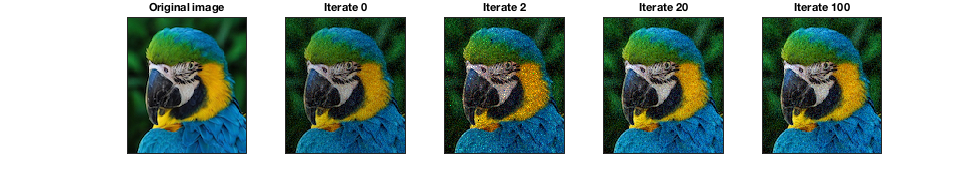
\includegraphics[scale=0.55]{parrot_signal_iterates} }
\hbox{\hspace{-1.7cm} 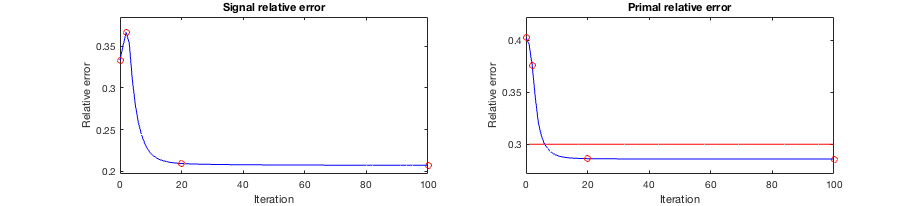
\includegraphics[scale=0.6]{parrot_signal_relative_error_2} }
\caption{Results from the first-order PLGD algorithm (Algorithm \ref{Alg:PGD}) applied to a test image separated into its three RGB channels.  Left: signal relative error $||xx^*- \mathbf{x}\mathbf{x}^*||_F / ||\mathbf{x}\mathbf{x}^*||_F$.  Right: primal relative error $||\caA(xx^*)-b||_2 /  ||b||_2$ with red line indicating primal feasibility.  Red circles denote the iterate signals pictured above.  Original signal is $128 \times 128$ pixels, with an oversampling of $L = 8$ and noise ratio $\epsilon_\rel = 0.30$.  Measurements use the mean of the three color channel values.}
\label{Fig:parrot_signal_relative_error_2}
\end{figure}
% experiments.figure.noisyimage_signal_relerr_various_saga_iterates

Figure \ref{Fig:parrot_signal_relative_error_2} demonstrates the tendency of Algorithm \ref{Alg:PGD} to make significant progress during early iterates.  When the same set of models in Figure \ref{Fig:parrot_signal_relative_error_2} were solved with wflow, the red channel converged to an infeasible solution (with primal residual $0.300068$), the green channel converged to a feasible solution (with primal residual $0.288473$), and the blue channel diverged.  





Table \ref{Tab:relative_errors_saga_vs_wflow} and Figure \ref{Fig:parrot_signal_relative_error_2} highlight the effectiveness of the first-order PLGD algorithm (Algorithm \ref{Alg:PGD}) for noisy phase retrieval problems.  
This algorithm is typically is more robust than wflow (Algorithm \ref{Alg:wflow}) and tends to recover signals successfully when there is minimal oversampling. 
Among the phase retrieval models and methods considered in this chapter, the PLGD model (\ref{Eqn:PLGD_ch2}) is the best suited for large-scale, unstructured noisy phase retrieval problems.
In the next two chapters we present the theory behind the PLGD model and develop a first-order algorithm for optimizing this model.



\newpage



\chapter{Gauge duality theory and the PhaseLift gauge dual model}	\label{Sec:PLGD}


\section{Introduction} 	\label{Subsec:PLGD-intro}

This chapter examines the PLGD model for solving the phase retrieval problem (\ref{Eqn:phase_retrieval}) and presents the gauge duality theory necessary for optimizing this model.  The PLGD model is the constrained eigenvalue optimization problem
\begin{equation*}
\begin{array}{ll}
	\min\limits_{\substack{y}}
					&	\lambda_1(\caA^* y)
						\\
	\st
					&	\langle b, y \rangle - \epsilon ||y||_2 \geq 1.
\end{array}
\end{equation*}


We begin in Section \ref{Subsec:PLGD-models_intro} by stating the PhaseLift primal (PLP) and gauge dual (PLGD) pair of models and reviewing key definitions.
Section \ref{Subsec:PLGD-models_intro} also states a few more general primal-gauge dual model pairs and provides a brief history of gauge duality theory.
In Section \ref{Subsec:PLGD-theory} we prove the gauge duality theorem (Theorem \ref{Thm:P-GD-inequality_pair_are_duals}) for a more general primal-gauge dual model pair and establish weak duality, strong duality, and optimality conditions for this pair.
Section \ref{Subsec:PLGD-opt_conds_primal_recovery} then returns to the PLP-PLGD pair, establishing key properties for optimizing the PLGD model and recovering a signal $x$ from a given dual variable $y$.  

All of the gauge properties and gauge duality results in this chapter were previously established in \cite{rockafellar1970convex}, \cite{DBLP:journals/mp/Freund87}, \cite{DBLP:journals/siamjo/FriedlanderMP14}, and \cite{DBLP:journals/siamsc/FriedlanderM16}.  Gauge functions were first analyzed in  \cite{rockafellar1970convex}.  Gauge duality was then introduced in \cite{DBLP:journals/mp/Freund87}, where the author focused on quadratic programming applications.  In \cite{DBLP:journals/siamjo/FriedlanderMP14}, the authors developed a broad set of antipolar calculus results for the analysis of gauge duality.  These results were then applied to the PLP-PLGD pair to develop a first-order method in \cite{DBLP:journals/siamsc/FriedlanderM16}.


Our contribution is to provide a self-contained, comprehensive treatment of gauge duality theory for the PLP-PLGD pair.  Prior to this treatment, the results in this chapter were spread throughout the original texts (\cite{rockafellar1970convex}, \cite{DBLP:journals/siamjo/FriedlanderMP14}, and \cite{DBLP:journals/siamsc/FriedlanderM16}), occasionally with differing notation or style.  In contrast, Section \ref{Subsec:PLGD-models_intro} provides a single notation and style which is used in Sections \ref{Subsec:PLGD-theory} and \ref{Subsec:PLGD-opt_conds_primal_recovery} to develop gauge duality theory for the PLP-PLGD pair.  The results of this chapter provide the theoretical foundation for developing a first-order optimization method for the PLGD model in Chapter \ref{Sec:PLGD_algo}.


\section{Definitions and primal-dual pairs}		\label{Subsec:PLGD-models_intro}



The PhaseLift primal semidefinite program (restated from (\ref{Eqn:PhaseLift}) in Section \ref{Subsubsec:phase_retrieval-unstructured}) and its gauge dual are
\begin{equation} \label{Eqn:PhaseLift-P-GD}
\begin{array}{lllllll}
	&	\min\limits_{\substack{X}}
		&	||X||_1 = \sum\limits_{\substack{i=1}}^{\substack{n}} \sigma_i(X)
			&
				&	\min\limits_{\substack{y}}
					&	\lambda_1(\caA^* y)
						\\
\textnormal{(PLP)}
	&	\st
		& 	|| \caA (X) - b || \leq \epsilon
			&	\hspace{0.4cm} 	\textnormal{(PLGD)}
				&	\st
					&	\langle b, y \rangle - \epsilon ||y|| \geq 1.
						\\

	&
		&	X \succeq 0

\end{array}
\end{equation}
This section places the PLP-PLGD pair (\ref{Eqn:PhaseLift-P-GD}) in the context of gauge duality theory.  We begin by discussing definitions and basic properties which are relevant to gauge duality theory. 
We then take a moment to highlight some parallels between gauge duality and Lagrange duality before closing with a summary of major developments in gauge duality theory.  
Along the way, we present three additional, more general primal-gauge dual models which have PLP-PLGD (\ref{Eqn:PhaseLift-P-GD}) as a special case.  Two of these models are then used in Section \ref{Subsec:PLGD-theory} to develop the theory which establishes the gauge duality of the pair (\ref{Eqn:PhaseLift-P-GD}).




The PLP-PLGD pair (\ref{Eqn:PhaseLift-P-GD}) are examples of a more general primal-gauge dual pair which we define as the \textit{nonlinearly-constrained} pair
\begin{equation} 			\label{Eqn:PhaseLift_P_GD_nonlinear_form}
\begin{array}{lllllll}
	&	\min\limits_{\substack{x \in \caX}}
		&	\kappa(x)
			&
				&	\min\limits_{\substack{z \in \caX}}
					&	\kappa^\circ(z)
						\\
\textnormal{(P-nonlin)}
	&	\st
		& 	x \in \caC
			&	\hspace{3cm} 	\textnormal{(GD-nonlin)}
				&	\st
					&	z \in \caC'.
\end{array}
\end{equation}
Here, $\caC$ and $\caC'$ are subsets of $\caX$, a finite-dimensional Euclidean space.  The set $\caC'$ is the \textit{antipolar} of $\caC$, defined as
\begin{equation}  			\label{Def:antipolar_set}
\caC' = \{ z \ | \ \langle x, z \rangle \geq 1 \ \forall x \in \caC \}.
\end{equation}
This is in contrast to the \textit{polar} of $\caC$, which is defined as
\begin{equation} 			\label{Def:polar}
\caC^\circ = \left\{ z \ | \ \langle x, z \rangle \leq 1 \ \forall x \in \caC \right\}.
\end{equation}
Although we refer to the primal-gauge dual pair (\ref{Eqn:PhaseLift_P_GD_nonlinear_form}) as nonlinear, we are primarily concerned with closed, convex sets $\caC$ which do not contain the origin (e.g., the PLP (\ref{Eqn:PhaseLift-P-GD}) constraint set when $\epsilon < ||b||$).  
Note that gauge dual models with linear constraints which do not include the origin are a subset of the models described by (\ref{Eqn:PhaseLift_P_GD_nonlinear_form}).

The functions $\kappa, \kappa^\circ : \caX \rightarrow \bbR \cup \{+\infty\}$ in (\ref{Eqn:PhaseLift_P_GD_nonlinear_form}) are \textit{gauge} functions, meaning they are convex, nonnegative, positively homogeneous ($\kappa(\alpha x) = \alpha \kappa(x)$ for all $\alpha > 0$), and vanish at the origin.  Gauge functions generalize the notion of norms, allowing for flexibility in modeling the phase retrieval problem.  In the PLP model for instance, the Schatten $1$-norm $\kappa(X) := || X ||_1$ and  vector $2$-norm $\rho(y) := ||y||$ are both gauges.

Given a gauge function $\kappa$, the \textit{polar} of this function is the function $\kappa^\circ$ that most tightly satisfies the inequality
\begin{equation}  			\label{Def:polar_function_1}
\begin{array}{ll}
	\langle x, z \rangle \leq \kappa(x) \kappa^\circ(z)
			&	\forall x \in \textnormal{dom} \ \kappa, \ \forall z \in \textnormal{dom} \ \kappa^\circ.
\end{array}
\end{equation}
Equivalently, the polar may be defined as \cite[Section 15]{rockafellar1970convex}
\begin{equation}  			\label{Def:polar_function_2}
\kappa^\circ(z) = \inf \left\{ \mu > 0 \ | \ \langle x, z \rangle \leq \mu \kappa(x) \ \forall x \right\}.
\end{equation}
Note that the polar is a generalization of the \textit{dual norm}, which is defined as
\begin{equation}			\label{Def:dual_norm}
||z||_* = \sup_{x} \halfspace \{ \halfspace  \langle x, z \rangle \ | \ ||x|| \leq 1 \}.
\end{equation}
The \textit{preimage} of a linear operator $A: \caX \rightarrow \caY$ over the set $\caS \subseteq \caY$ is defined as 
\begin{equation} 			\label{Def:preimage}
A^{-1} \caS = \{ x \in \caX \ | \ Ax \in \caS \}.
\end{equation}
The \textit{closure} of a set $\caS \subseteq \caX$ is denoted $\textnormal{cl}(\caS)$. The \textit{affine hull} of $\caS$ is the set of all affine combinations of elements of $\caS$, or
\begin{equation}			\label{Def:affine_hull}
\text{aff}(\caS) = \left\{ \sum_{i=1}^k \alpha_i x_i \ \middle| \ k > 0, \ x_i \in \caS, \ \alpha_i \in \bbR, \ \sum_{i=1}^k \alpha_i = 1 \right\}.
\end{equation}
The \textit{relative interior} of $\caS$, denoted $\textnormal{ri}(\caS)$, is the interior within the affine hull of $\caS$, i.e.,
\begin{equation}			\label{Def:relative_interior}
\text{ri}(\caS) = \{ x \in \caS \ | \ \exists \ \epsilon > 0, \ B_\epsilon(x) \cap \text{aff}(\caS) \subseteq \caS  \},
\end{equation}
where $B_\epsilon(x)$ is a ball of radius $\epsilon$ centered at $x$.
The \textit{support} function $\sigma_\caC$ of a nonempty convex set $\caC$ is defined as
\begin{equation}		\label{Def:support_function}
\sigma_\caC(z) = \sup_{x \in \caC} \langle x, z \rangle.
\end{equation}
And the \textit{Minkowski} function $\gamma_\caC$ is defined as
\begin{equation}			\label{Def:Minkowski_function}
\gamma_\caC(x) = \inf \left\{ \lambda \geq 0 \ | \ x \in \lambda \caC  \right\}.
\end{equation}
If there is no $\lambda$ such that $\lambda x \in \caC$, then $\gamma_\caC(x) = + \infty$.  Note that any gauge $\kappa$ is a Minkowski function $\gamma_\caC$ for $\caC = \{ x \ | \ \kappa(x) \leq 1 \}$ \cite[Section 15]{rockafellar1970convex}.  Given a function $f : \caX \rightarrow \bbR \cup \{+\infty\}$, the \textit{epigraph} of $f$ is defined as
\begin{equation}		\label{Eqn:epigraph}
\textnormal{epi}(f) = \left\{ (x, \tau) \ | \ f(x) \leq \tau  \right\}.
\end{equation}
Note that $f$ is convex if and only if $\textnormal{epi}(f)$ is convex \cite[Section 7]{rockafellar1970convex}.  Thus the function $f$ is said to be \textit{closed} if $\textnormal{epi}(f)$ is closed.  Additionally, $f$ is closed if and only if it is lower-semicontinuous (that is, $\liminf_{x \rightarrow x_0} f(x) \geq f(x_0)$ for all $x_0$ in $\textnormal{dom}(f)$) \cite[Section 7]{rockafellar1970convex}.  Also, $f$ is \textit{proper} if the domain of $f$, $\textnormal{dom}(f) = \{ x \ | \ f(x) < +\infty \}$ is nonempty.  

If $\kappa$ is a closed gauge, then its polar may also be expressed as \cite[Section 15]{rockafellar1970convex}
\begin{equation}			\label{Def:polar_function_3}
\kappa^\circ(z) = \sup\limits_x \left\{ \langle x, z \rangle \ | \ \kappa(x) \leq 1 \right\},
\end{equation}
again highlighting the fact that the polar function is a generalization of the dual norm (\ref{Def:dual_norm}).  
Additionally, if $\kappa$ is also positive everywhere except at the origin then its polar may also be defined as \cite[Section 15]{rockafellar1970convex}
\begin{equation}			\label{Def:polar_function_4}
\kappa^\circ(z) = \sup\limits_x \left\{ \frac{\langle x, z \rangle}{\kappa(x)} \right\}.
\end{equation}





Given the gauge duality notation discussed above, we take a moment to contrast gauge duality with the much more common Lagrange duality.  Whereas gauge duality involves multiplicative duality transformations, Lagrange duality is additive in nature.  The reader may see \cite[Chapter 5]{boyd2004convex} for a comprehensive introduction to Lagrange duality, and \cite[Section 28]{rockafellar1970convex} or \cite[Chapter 2]{ben2001lectures} for a treatment of Lagrange duality theory.


Given P-nonlin, the primal model in (\ref{Eqn:PhaseLift_P_GD_nonlinear_form}), we see that its gauge dual GD-nonlin can be stated simply using the polar function $\kappa^\circ$ and the antipolar set $\caC'$.  
Similarly, the Lagrange dual of P-nonlin can be described using the appropriate function and set transformations.  Given a function $f : \caX \rightarrow \bbR \ \cup \ \{\pm \infty\}$, the \textit{convex conjugate} $f^*$ is defined as the function that most tightly satisfies the inequality
\begin{equation} 			\label{Def:conjugate_function_1}
\begin{array}{ll}
	\langle x, z \rangle \leq f(x) + f^*(z)
			&	\forall x \in \textnormal{dom} \ f, \ \forall z \in \textnormal{dom} \ f^*.
\end{array}
\end{equation}
Equivalently, the convex conjugate may be defined as \cite[Section 12]{rockafellar1970convex}
\begin{equation} 			\label{Def:conjugate_function_2}
f^*(z) = \sup_x \left\{ \langle x, z \rangle - f(x)  \right\}.
\end{equation}
We see that (\ref{Def:conjugate_function_1}) and (\ref{Def:conjugate_function_2}) are the additive analogs of the polar function definitions (\ref{Def:polar_function_1}) and (\ref{Def:polar_function_4}), respectively.  Additionally, for a set $\caS \subseteq \caX$, the \textit{dual cone} is defined as
\begin{equation}			\label{Def:dual_cone}
\caS^* = \{ z \ | \ \langle x, z \rangle \leq 0 \ \forall x \in \caS \}.
\end{equation}
Given the convex conjugate $\kappa^*$ and the dual cone $\caC^*$, the Lagrange dual D-nonlin and gauge dual GD-nonlin both have the simple forms
\begin{equation} 			
\begin{array}{lllllll}
	&	\max\limits_{\substack{z}}
		&	-\kappa^*(z)
			&
				&	\min\limits_{\substack{z \in \caX}}
					&	\kappa^\circ(z)
						\\
\textnormal{(D-nonlin)}
	&	\st
		&z \in \caC^*
			&	\hspace{2cm} 	\textnormal{(GD-nonlin)}
				&	\st
					&	z \in \caC'.
\end{array}
\end{equation}
Note that Lagrange duality applies for any function $f : \caX \rightarrow \bbR \ \cup \ \{\pm \infty\}$ and set $\caS \subseteq \caX$.  Thus Lagrange duality has been studied thoroughly and applied extensively (e.g., see \cite[Chapter 5]{boyd2004convex}).  In contrast, gauge duality places specific restrictions on the objective function and constraint set.  As a result,  the development of gauge duality theory has a brief, sporadic history.






In 1970, Rockafellar thoroughly analyzed gauge functions and their polars \cite[Part III]{rockafellar1970convex}.  
The concept of gauge duality was then introduced by Freund in 1987 \cite{DBLP:journals/mp/Freund87}.  
This seminal work focused primarily on the \textit{linearly-constrained} primal and gauge dual pair
\begin{equation} 			\label{Eqn:PhaseLift_P_GD_linear_form}
\begin{array}{lllllll}
	&	\min\limits_{\substack{x \in \caX}}
		&	\kappa(x)
			&
				&	\min\limits_{\substack{y \in \caY}}
					&	\kappa^\circ(A^*y)
						\\
\textnormal{(P-lin)}
	&	\st
		& 	Ax=b
			&	\hspace{3cm} 	\textnormal{(GD-lin)}
				&	\st
					&	\langle b, y \rangle = 1.
\end{array}
\end{equation}
Here $A : \caX \rightarrow \caY$ is a linear operator over finite-dimensional Euclidean spaces. 
As with Lagrange duality, if the primal constraint is replaced with $Ax \geq b$ then the gauge dual also includes the constraint $y \geq 0$.  
Freund develops strong duality and optimality conditions for the pair (\ref{Eqn:PhaseLift_P_GD_linear_form}) based on polarity relationships for sets and gauge functions.  
His work also establishes these conditions for the nonlinear pair (\ref{Eqn:PhaseLift_P_GD_nonlinear_form}).  
In this case, his work requires $\caX$ and $\caY$ to be \textit{ray-like} (meaning that for all $x, y \in \caX$ we have $x + \alpha y \in \caX$ for all $\alpha \geq 0$).  
The addition of the ray-like property to $\caX$ (along with closed, convex, and containing the origin) guarantees $\caX'' = \caX$.


Gauge duality theory was revisited in \cite{DBLP:journals/siamjo/FriedlanderMP14}, where the authors consider the \textit{inequality-constrained} primal and gauge dual pair
\begin{equation} 			\label{Eqn:PhaseLift_P_GD_inequality_form}
\begin{array}{lllllll}
	&	\min\limits_{\substack{x \in \caX}}
		&	\kappa(x)
			&
				&	\min\limits_{\substack{y \in \caY}}
					&	\kappa^\circ(A^*y)
						\\
\textnormal{(P-ineq)}
	&	\st
		& 	\rho(Ax-b) \leq \epsilon
			&	\hspace{0.4cm} 	\textnormal{(GD-ineq)}
				&	\st
					&	\langle b, y \rangle - \epsilon \rho^\circ(y) \geq 1.
\end{array}
\end{equation}
As we will see in Section \ref{Subsec:PLGD-opt_conds_primal_recovery}, the PLP-PLGD pair (\ref{Eqn:PhaseLift-P-GD}) pair is recovered from (\ref{Eqn:PhaseLift_P_GD_inequality_form}) when we set $\kappa(X) = ||X||_1 + \delta_{(\cdot) \succeq 0}(X)$ and $\rho(y) = ||y||$.  The authors of \cite{DBLP:journals/siamjo/FriedlanderMP14} develop an antipolar calculus to determine the antipolar for sets like $\{ y \ | \ \rho(Ax-b) \leq \epsilon \}$ and use this calculus rather than polarity relations to derive the gauge dual pair (\ref{Eqn:PhaseLift_P_GD_inequality_form}) and establish conditions such as those for strong duality.  Additionally, this antipolar calculus allows the authors to drop the requirement that the sets $\caX$ and $\caY$ are ray-like.

In contrast to the antipolar calculus framework, the authors of \cite{aravkin2017foundations} develop gauge duality through a perturbation framework.  This even broader setting frames gauge duality as a product of Fenchel-Rockafellar duality, allowing the consideration of gauge duality for 
general nonnegative convex functions.









\section{Theory for linearly and nonlinearly constrained models} 			\label{Subsec:PLGD-theory}






In this section we develop gauge duality theory for the inequality-constrained primal and gauge dual pair (\ref{Eqn:PhaseLift_P_GD_inequality_form}).  We begin by establishing the propositions necessary to show the gauge duality of (\ref{Eqn:PhaseLift_P_GD_inequality_form}) is a consequence of the duality of both the nonlinear (\ref{Eqn:PhaseLift_P_GD_nonlinear_form}) and linear (\ref{Eqn:PhaseLift_P_GD_linear_form}) models.  This two-track proof strategy as depicted in Figure \ref{Fig:gauge_duality_thm_flowchart} leads to Theorem \ref{Thm:P-GD-inequality_pair_are_duals}, (i) and (ii), respectively.
\begin{figure}[H] 
\centering
\hspace{0cm}
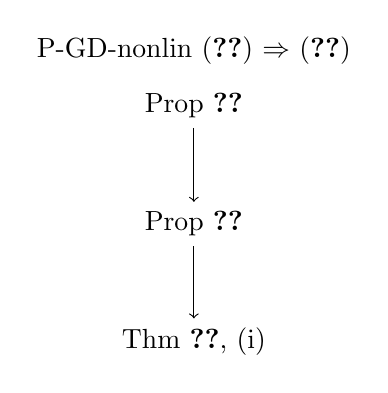
\begin{tikzpicture} 
	\node (1) at (0,3.7) {P-GD-nonlin (\ref{Eqn:PhaseLift_P_GD_nonlinear_form}) $\Rightarrow$ (\ref{Eqn:PhaseLift_P_GD_inequality_form})};
 	\node (2) at (0,3) {Prop \ref{Prop:antipolar_set_equalities}};
	\node (3) at (0,1.5) {Prop \ref{Prop:antipolar_of_primal_phase_retrieval}};
	\node (4) at (0,0) {Thm \ref{Thm:P-GD-inequality_pair_are_duals}, (i)};
	\draw[->] (2) -- (3);
	\draw[->] (3) -- (4);
\end{tikzpicture}
\hspace{1cm}
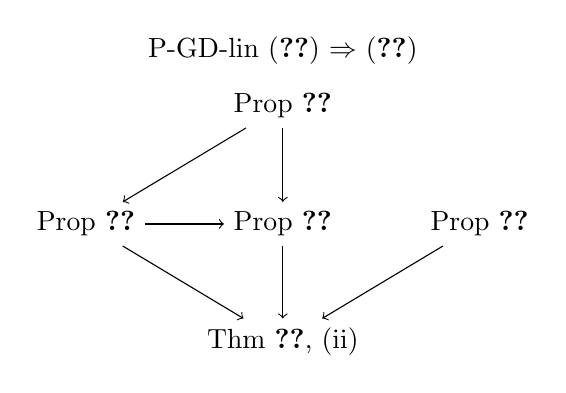
\begin{tikzpicture}
	\node (6) at (2.5,3.7) {P-GD-lin (\ref{Eqn:PhaseLift_P_GD_linear_form}) $\Rightarrow$ (\ref{Eqn:PhaseLift_P_GD_inequality_form})};
	\node (1) at (2.5,3) {Prop \ref{Prop:P-GD-Minkowski_set_unique}};
	\node (2) at (0,1.5) {Prop \ref{Prop:P-GD-polar_of_sum_of_gauges_sets_equal}};
	\node (3) at (2.5,1.5) {Prop \ref{Prop:P-GD-polar_of_sum_of_gauges}};
	\node (4) at (5,1.5) {Prop \ref{Prop:P-GD-indicator_epigraph_polar}};
	\node (5) at (2.5,0) {Thm \ref{Thm:P-GD-inequality_pair_are_duals}, (ii)};
	\draw[->] (1) -- (2);
	\draw[->] (1) -- (3);
	\draw[->] (2) -- (3);
	\draw[->] (2) -- (5);
	\draw[->] (3) -- (5);
	\draw[->] (4) -- (5);
\end{tikzpicture}
\caption{Dependency chart for proofs (i) and (ii) of Theorem \ref{Thm:P-GD-inequality_pair_are_duals} which establish the gauge duality of P-GD-ineq (\ref{Eqn:PhaseLift_P_GD_inequality_form}).
  	}
\label{Fig:gauge_duality_thm_flowchart}
\end{figure}

Following Theorem \ref{Thm:P-GD-inequality_pair_are_duals} we establish weak duality, strong duality, and optimality conditions for (\ref{Eqn:PhaseLift_P_GD_inequality_form}).  In Section \ref{Subsec:PLGD-opt_conds_primal_recovery} we will return to the PhaseLift model (\ref{Eqn:PhaseLift-P-GD}), where the optimality conditions in this section provide a method for recovery of a primal signal $x$ from a dual variable $y$.


The results in this section are based on \cite{rockafellar1970convex}, \cite{DBLP:journals/mp/Freund87}, and especially \cite{DBLP:journals/siamjo/FriedlanderMP14}, and rely on the analysis of polarity relations rather than perturbation analysis as discussed in \cite{aravkin2017foundations}.    In particular, the two-track proof strategy depicted in Figure \ref{Fig:gauge_duality_thm_flowchart} was first developed in \cite{DBLP:journals/siamjo/FriedlanderMP14} as part of a larger treatment of antipolar calculus, and refers to \cite{rockafellar1970convex} for more elementary results (e.g., Propositions \ref{Prop:P-GD-Minkowski_set_unique}, \ref{Prop:P-GD-polar_of_sum_of_gauges_sets_equal}, and \ref{Prop:P-GD-indicator_epigraph_polar}).  This section provides a self-contained development of gauge duality for (\ref{Eqn:PhaseLift_P_GD_inequality_form}).





The next two propositions are used in Theorem \ref{Thm:P-GD-inequality_pair_are_duals}, (i) to show the inequality pair (\ref{Eqn:PhaseLift_P_GD_inequality_form}) is an instance of the nonlinear pair (\ref{Eqn:PhaseLift_P_GD_nonlinear_form}).  Since (\ref{Eqn:PhaseLift_P_GD_inequality_form}) allows for the constraint set $\caC$ to be any closed, convex set not containing the origin, we must simply establish the antipolar of the constraint set $\caC = \{ x \ | \rho(Ax-b) \leq \epsilon\}$.  We begin by showing how linear and polar transformations on $\caC$ commute under certain assumptions.





\begin{prop}		\label{Prop:antipolar_set_equalities}
Let $\caX$ and $\caY$ be finite-dimensional Euclidean spaces, $\caC \subseteq \caX$ a closed, convex set which does not contain the origin, $A : \caX \rightarrow \caY$ a linear operator, and $A^* : \caY \rightarrow \caX$ its adjoint.
%(so $\langle A^*y, x\rangle = \langle y, Ax \rangle$ for all $x \in \caX$ and $y \in \caY$).    
Then
\begin{equation}		\label{Eqn:antipolar_set_equalities_1}
\begin{array}{rll}
\left( A \caC \right)' & = & 	\left( A^* \right)^{-1} \caC' .
\end{array}
\end{equation}

Additionally, assume $\caC$ is polyhedral or $\textnormal{ri}(\caC) \cap \textnormal{range}(A) \neq \emptyset$, and $A^{-1}\caC$ is not empty.  
Then $( A^{-1} \caC)'$ is nonempty and the following set equality holds
% (A\caC)'	&	=	&	\left( A^* \right)^{-1} \caC'	\\
\begin{equation}		\label{Eqn:antipolar_set_equalities_2}
\begin{array}{rll}
\left( A^{-1} \caC \right)' & = &  A^* \caC' .
\end{array}
\end{equation}
\end{prop}
\begin{proof}
The first result is proved in \cite[Proposition 3.3]{DBLP:journals/siamjo/FriedlanderMP14} and the second in \cite[Proposition 3.4, 3.5]{DBLP:journals/siamjo/FriedlanderMP14}.
\end{proof}


The previous propositions allows us to construct the antipolar of the constraint set $\caC = \{ x \ | \ \rho(Ax-b) \leq \epsilon \}$ in Proposition \ref{Prop:antipolar_of_primal_phase_retrieval}.

\begin{prop}		\label{Prop:antipolar_of_primal_phase_retrieval}
Let $\caX$ and $\caY$ be finite-dimensional Euclidean spaces, $A : \caX \rightarrow \caY$ a linear operator, and $A^* : \caY \rightarrow \caX$ its adjoint.  Let $\caC = \{ x \ | \ \rho(Ax-b) \leq \epsilon \}$ with $0 < \epsilon < \rho(b)$.  Also assume $\textnormal{ri}(\caC) \cap \textnormal{range}(A)$ and $A^{-1}\caC$ are not empty. Then
\begin{equation}			\label{Eqn:antipolar_of_primal_phase_retrieval}
\caC' = \left\{ A^*y \ | \ \langle b, y \rangle - \epsilon \rho^\circ(y) \geq 1  \right\}.	
\end{equation}
\end{prop}
\begin{proof}
Since the arguments of $\rho$ lie in $\caY$, we first consider the antipolar of $\caD = A\caC \subseteq \caY$ to establish the constraint $\langle b, y \rangle - \epsilon \rho^\circ(y) \geq 1$.  Note that $y \in \caD'$ is equivalent to $\langle Ax, y \rangle \geq 1$ for all $Ax \in A\caC$.  This is again equivalent to
\begin{equation}				\label{Eqn:antipolar_eqn_for_proof_1}
\langle b - Ax, y \rangle \leq \langle b, y \rangle - 1 \ \forall x \ \textnormal{such that} \ \rho(Ax-b) \leq \epsilon.
\end{equation}
Next apply definition (\ref{Def:polar_function_3}) for the antipolar $\rho^\circ$ and take the supremum over $u = \frac{b-Ax}{\epsilon}$, giving 
\begin{equation}  		\label{Eqn:antipolar_eqn_for_proof_2}
\begin{array}{lll}
\epsilon \rho^\circ(y) 	&	=	&	\epsilon \sup\limits_{\substack{u}} \left\{ \langle u, y \rangle \ | \ \rho(u) \leq 1, \ u = \frac{b-Ax}{\epsilon}  \right\} 	\\
	&	= 	&  \sup\limits_{\substack{x}} \left\{ \langle b - Ax, y \rangle \ | \ \rho\left(\frac{b-Ax}{\epsilon}\right) \leq 1  \right\} \\
		&	= 	&  \sup\limits_{\substack{x}} \left\{ \langle b - Ax, y \rangle \ | \ \rho(b-Ax) \leq \epsilon  \right\},
\end{array}
\end{equation}
where the last equality uses the postive homogeneity of the gauge $\rho$.  Using equation (\ref{Eqn:antipolar_eqn_for_proof_2}), we see that equation (\ref{Eqn:antipolar_eqn_for_proof_1}) is equivalent to the desired constraint $\epsilon \rho^\circ(y) \leq  \langle b, y \rangle - 1$.  Thus $\caD' = \{ y \ | \ \langle b, y \rangle - \epsilon \rho^\circ(y) \geq 1 \}$.

Finally, note that $\caC$ and $\caC'$ both lie in $\caX$, while $\caD = A\caC$ and $\caD'$ lie in $\caY$.  Then by Proposition \ref{Prop:antipolar_set_equalities}, the antipolar $\caC'$ has the form
\begin{equation}
\begin{array}{lll}
\caC' = \left(A^{-1} \caD \right)'	& =  &	A^* \caD' 	\\
	&	=	&		\left\{ A^*y 	\	|	\ \langle b, y \rangle - \epsilon \rho^\circ(y) \geq 1  \right\}.
\end{array}
\end{equation}
\end{proof}





The next four propositions allow us to derive the inequality-constrained primal-gauge dual pair (\ref{Eqn:PhaseLift_P_GD_inequality_form}) from the linearly-constrained pair (\ref{Eqn:PhaseLift_P_GD_linear_form}) by transforming the P-ineq model into a linearly-constrained gauge model of the form P-lin (see the dependency map in Figure \ref{Fig:gauge_duality_thm_flowchart} for reference).   
This process uses an indicator function to embed the constraint set $\caC = \{ x \ | \ \rho(Ax-b) \leq \epsilon\}$ into the primal objective function, resulting in a P-lin model (\ref{Eqn:PhaseLift_P_GD_linear_form}).  Finally, we determine the gauge dual of the resulting model using polar relations and properties established in Section \ref{Subsec:PLGD-models_intro}.


The first two propositions show that we may discuss the polar of a sum of gauges in terms of sets induced by Minkowski functions.  This allows us to determine the polar of a sum of gauges in Proposition \ref{Prop:P-GD-polar_of_sum_of_gauges}.

\begin{prop} 			\label{Prop:P-GD-Minkowski_set_unique}
Let $\caC \subseteq \caX$ be a closed, convex set containing the origin and $\kappa = \gamma_\caC$ the Minkowski function induced by $\caC$.  Then $\kappa$ is a gauge, $\caC = \{ x \ | \ \kappa(x) \leq 1 \}$, and $\caC$ is the unique closed, convex set containing the origin such that $\kappa = \gamma_\caC$.
\end{prop}
\begin{proof}
To verify that $\kappa$ is a gauge, first note that positive homogeneity and $\kappa(0) = 0$ are direct results of $\kappa$ being a Minkowski function.  To show convexity, let $x, y \in \caX$ and $0 \leq \alpha \leq 1$.  Then $x \in \kappa(x) \caC$ means $\alpha x \in \alpha \kappa(x) \caC$, and likewise $(1-\alpha) y \in (1-\alpha) \kappa(y) \caC$.  Thus $\alpha x + (1-\alpha)y \in (\alpha \kappa(x) + (1-\alpha) \kappa(y)) \caC$.  Then by the infimum of the Minkowski function, $\kappa(\alpha x + (1-\alpha) y) \leq \alpha \kappa(x) + (1-\alpha) \kappa(y)$ and $\kappa$ is convex.

Additionally, $\kappa(x) \leq 1$ is equivalent to $x \in \caC$, and thus $\caC =  \{ x \ | \ \kappa(x) \leq 1 \}$.

Finally, assume there is some closed, convex set $\caD \subseteq \caX$ such that $\kappa = \gamma_\caD$.  Then $\kappa(x) = \gamma_\caC(x) = \gamma_\caD(x) \leq 1$ is equivalent to $x$ being in both $\caC$ and $\caD$, since both sets are closed and convex. Likewise, $\kappa(x) > 1$ indicates $x$ is in neither set.  Thus $\caC = \caD$.

\end{proof}

\begin{prop} 			\label{Prop:P-GD-polar_of_sum_of_gauges_sets_equal}
Let $\kappa_1$ and $\kappa_2$ be gauges.  Let $\kappa(x_1, x_2) = \kappa_1(x_1) + \kappa_2(x_2)$, $\caC_1 = \{ z_1 \ | \ \kappa^\circ(z_1) \leq 1 \}$, $\caC_2 = \{ z_2 \ | \ \kappa^\circ(z_2) \leq 1 \}$, and $\caC = \{ (z_1, z_2) \ | \ \kappa^\circ(z_1, z_2) \leq 1 \}$. Then $\kappa$ and $\kappa^\circ$ are gauges, $\kappa^\circ = \gamma_\caC$, and $\caC = \caC_1 \times \caC_2$.
\end{prop}
\begin{proof}
Since $\kappa$ is the sum of gauges, it is also convex, nonnegative, positively homogeneous, and zero at the origin, and thus a gauge.  Then $\kappa^\circ$ is also a gauge and by Proposition \ref{Prop:P-GD-Minkowski_set_unique}, $\caC$ is the unique set such that $\kappa = \gamma_\caC$.
If $(z_1, z_2) \in \caC$, then $\langle x_1, z_1 \rangle + \langle x_2, z_2 \rangle \leq \kappa(x_1,x_2)\kappa^\circ(z_1,z_2) \leq  \kappa_1(x_1) + \kappa_2 (x_2)$ for all $x_1 \in \textnormal{dom}\ \kappa_1$ and $x_2 \in \textnormal{dom} \ \kappa_2$.  In particular, if $x_2 = 0$ then $\langle x_1, z_1 \rangle \leq \kappa_1(x_1)$ for all $x_1  \in \textnormal{dom}\ \kappa_1$, indicating $z_1 \in \caC_1$.  Similarly $z_2 \in \caC_2$ and thus $\caC_1 \times \caC_2 \subseteq \caC$.  For the reverse inclusion, $(z_1, z_2) \in \caC_1 \times \caC_2$ means $\langle x_1, z_1 \rangle \leq \kappa_1(x_1)$ for all $x_1 \in \textnormal{dom}\ \kappa_1$ and $\langle x_2, z_2 \rangle \leq \kappa_2(x_2)$ for all $x_2 \in \textnormal{dom}\ \kappa_2$.  Adding these inequalities, we have $\langle x_1, z_1 \rangle + \langle x_2, z_2 \rangle \leq \kappa_1(x_1) + \kappa_2 (x_2)$ for all $x_1 \in \textnormal{dom}\ \kappa_1$ and $x_2  \in \textnormal{dom}\ \kappa_2$, and thus $\caC = \caC_1 \times \caC_2$.
\end{proof}


Given the two propositions above, we now show that the polar of a sum of gauges is the max of the set of polars.

\begin{prop}			\label{Prop:P-GD-polar_of_sum_of_gauges}
Let $\kappa_1$ and $\kappa_2$ be gauges.  Then the sum $\kappa(x_1, x_2) := \kappa_1(x_1) + \kappa_2(x_2)$ is a guage and has the polar
\begin{equation}			\label{Eqn:polar_of_sum_of_gauges}
\kappa^\circ(z_1, z_2) = \max \left\{ \halfspace \kappa^\circ(z_1), \ \kappa_2^\circ(z_2) \right\}.
\end{equation}
\end{prop}
\begin{proof}
Proposition \ref{Prop:P-GD-polar_of_sum_of_gauges_sets_equal} shows $\kappa$ and its polar $\kappa^\circ$ are gauges.  Setting $\caC_1 = \{ z_1 \ | \ \kappa^\circ(z_1) \leq 1 \}$, $\caC_2 = \{ z_2 \ | \ \kappa^\circ(z_2) \leq 1 \}$, and $\caC = \{ (z_1, z_2) \ | \ \kappa^\circ(z_1, z_2) \leq 1 \}$, we may express the gauge polars as Minkowski functions $\kappa_1^\circ = \gamma_{\caC_1}$, $\kappa_2^\circ = \gamma_{\caC_2}$, and $\kappa^\circ = \gamma_{\caC}$.  
Since $\caC_1$, $\caC_2$, and $\caC$ are closed, convex sets containing the origin, Proposition \ref{Prop:P-GD-Minkowski_set_unique} tells us these are the unique sets defining $\kappa_1^\circ$, $\kappa_2^\circ$, and $\kappa^\circ$.  Additionally, Proposition \ref{Prop:P-GD-polar_of_sum_of_gauges_sets_equal} implies $\caC = \caC_1 \times \caC_2$ and $\kappa^\circ(z_1, z_2) =	\gamma_{\caC}(z_1, z_2) 	=	\gamma_{\caC_1 \times \caC_2}(z_1, z_2)$.


Then we have
\begin{equation}
\begin{array}{rll}
\kappa^\circ(z_1, z_2)	  & =	&	\gamma_{\caC_1 \times \caC_2}(z_1, z_2)	\\
	&	=	&	\inf \left\{ \halfspace \lambda \geq 0 \ | \ z_1 \in \lambda \caC_1, \ z_2 \in \lambda \caC_2 \right\} \\
	&	=	&	\max \left\{ \halfspace \inf \{ \lambda \geq 0 \ | \ z_1 \in \lambda \caC_1 \}, 
									\ \inf \{ \lambda \geq 0 \ | \ z_2 \in \lambda \caC_2 \} 	\right\}	\\
	&	=	&	\max \left\{ \halfspace \gamma_{\caC_1}(z_1), \ \gamma_{\caC_1}(z_2) \right\}	\\
	&	=	&	\max \left\{ \halfspace \kappa_1^\circ(z_1), \ \kappa_2^\circ(z_2) \right\}.
\end{array}
\end{equation}
\end{proof}


The following proposition establishes two equalities which allow us to compute the polar of an objective function which includes an indicator function.  This strategy allows us to embed the inequality $\rho(Ax-b) \leq \epsilon$ from (\ref{Eqn:PhaseLift_P_GD_inequality_form}) into the objective function of (\ref{Eqn:PhaseLift_P_GD_linear_form}) in the proof of Theorem \ref{Thm:P-GD-inequality_pair_are_duals}, (ii).


\begin{prop}				\label{Prop:P-GD-indicator_epigraph_polar}
Let $\rho$ be a gauge.  Then for all $y \in \caX$ and $\tau \geq 0$ the following equalities hold.
\begin{enumerate}[(i)]
\item
 $\left( \delta_{\textnormal{epi} \halfspace \rho} \right)^\circ(y, \tau) = \delta_{\left(  \textnormal{epi} \halfspace \rho \right)^\circ} (y, \tau)$,
\item
$\delta_{\left( \epi \halfspace \rho \right)^\circ} (y, \tau) = \delta_{\epi \left( \rho^\circ \right)}(y, -\tau)$.
\end{enumerate}
\end{prop}
\begin{proof}
To show (i) holds, consider the expansion of the expressions
\begin{equation*}
\begin{array}{rll}
\left( \delta_{\textnormal{epi} \halfspace \rho} \right)^\circ(y, \tau) 
	&	= 
			&	 \inf \left\{ \mu > 0 \ | \ \langle (x, \sigma), (y, \tau) \rangle \leq \mu \delta_{\epi \halfspace \rho}(x, \sigma) \ \ \forall (x, \sigma) \right\},
					\\
\delta_{\left( \epi \halfspace \rho \right)^\circ} (y, \tau) 
	&	= 
			&	\begin{cases}
						0 	&\textnormal{if } \langle (x, \sigma) , (y, \tau) \rangle \leq 1 \ \ \forall (x, \sigma) \in \epi \halfspace \rho \\
						+\infty	&\textnormal{else}.
				\end{cases}	
\end{array}
\end{equation*}
Note that the value of $\delta_{\left(  \textnormal{epi} \halfspace \rho \right)^\circ} (y, \tau)$ is either $0$ or $+\infty$.  If $\delta_{\left(  \textnormal{epi} \halfspace \rho \right)^\circ} (y, \tau) = 0$, then $\langle (x, \sigma), (y, \tau) \rangle  \leq 1$ for all $(x, \sigma) \in \epi \halfspace \rho$.  Since $\rho$ is a gauge, $(x, \sigma) \in \epi \halfspace \rho$ is equivalent to $\rho(\alpha x) \leq \alpha \sigma$ for all $\alpha > 0$.  Then $(\alpha x, \alpha \sigma) \in \epi \halfspace \rho$ for all $\alpha > 0$.  Dividing the inequality by $\alpha$ and letting $\alpha$ approach infinity, we have
\begin{equation*}
\langle (x, \sigma), (y, \tau) \rangle \leq \lim\limits_{\substack{\alpha \rightarrow +\infty}} \frac{1}{\alpha} = 0 \ \ \textnormal{for all} \ (x, \alpha) \in \epi \halfspace \rho.
\end{equation*}
Thus $\left( \delta_{\textnormal{epi} \halfspace \rho} \right)^\circ(y, \tau)  = 0$.  On the other hand, if $\delta_{\left(  \textnormal{epi} \halfspace \rho \right)^\circ} (y, \tau) = +\infty$ then there is some $(x, \sigma) \in \epi \halfspace \rho$ with $\langle (x, \sigma) , (y, \tau) \rangle > 1$.  Then $\delta_{\epi \halfspace \rho}(x, \sigma) = 0$ and there is no $\mu >0$ such that $\langle (x, \sigma), (y, \tau) \rangle \leq \mu \delta_{\epi \halfspace \rho}(x, \sigma)$.  Thus $\left( \delta_{\textnormal{epi} \halfspace \rho} \right)^\circ(y, \tau)  = +\infty$.

To show (ii) holds, we have the following set of equivalences
\begin{equation*}
\begin{array}{rll}
(y, \tau) \in \left( \epi \halfspace \rho \right)^\circ
	&	\iff	&  \langle (x, \sigma), (y, \tau) \rangle \leq 1 \ \ \forall (x, \sigma) \in  \epi (\rho)
			\\
	&	\iff	&	 \langle (x, \sigma), (y, \tau) \rangle \leq 0 \ \ \forall x \text{ and } \rho(x) \leq \sigma
			\\
	&	\iff	&	\langle x, y \rangle \leq -\tau \rho(x) \ \ \forall x
			\\
	&	\iff	&	\rho^\circ(y) = \inf \left\{ \mu > 0 \ | \ \langle x, y \rangle \leq \mu \rho(x) \ \ \forall x \right\} \leq - \tau
			\\
		&	\iff	&	(y, -\tau)  \in \epi (\rho^\circ).
\end{array}
\end{equation*}
Here, the second equivalence was established in the proof of (i) and the third comes from setting $\sigma$ as the minimal value $\sigma = \rho(x)$.  Thus $\delta_{\left( \epi \halfspace \rho \right)^\circ} (y, \tau) = \delta_{\epi \left( \rho^\circ \right)}(y, -\tau)$.
\end{proof}


xxx here



We are now prepared to prove the essential results which underly our phase retrieval method and signal recovery strategy.  We begin with the following gauge duality result.

\begin{theorem} 				\label{Thm:P-GD-inequality_pair_are_duals}
Let P-ineq and GD-ineq be the inequality-constrained pair of models from (\ref{Eqn:PhaseLift_P_GD_inequality_form}).  Also let $\caC = \{ x \ | \ \rho(Ax-b) \leq \epsilon \}$ with $0 < \epsilon < \rho(b)$ and assume $\textnormal{ri}(\caC) \cap \textnormal{range}(A)$ and $A^{-1}\caC$ are not empty.  Then the model GD-ineq is the gauge dual of the primal P-ineq based on the gauge duality of 
\begin{enumerate}[(i)]
\item
the nonlinear gauge dual pair (\ref{Eqn:PhaseLift_P_GD_nonlinear_form}), and
\item
the linear gauge dual pair (\ref{Eqn:PhaseLift_P_GD_linear_form}).
\end{enumerate}
\end{theorem}


\begin{proof}
Item (i) is a direct result of Proposition \ref{Prop:antipolar_of_primal_phase_retrieval}, which gives the antipolar set $\caC' = \left\{ A^*y \ | \ \langle b, y \rangle - \epsilon \rho^\circ(y) \geq 1  \right\}$.  As a result, the argument of the GD-nonlin objective $\kappa^\circ$ is $A^*y$ and GD-ineq is equivalent to GD-nonlin.

To prove item (ii), we must first express P-ineq as a linear gauge model of the form P-lin.  Define the function $\phi(x, r, \sigma) = \kappa(x) + \delta_{\epi \halfspace \rho}(r, \sigma)$.  Since the epigraph of a gauge is closed under positive scaling, the indicator function $\delta_{\epi \halfspace \rho}$ is a gauge.  By Proposition \ref{Prop:P-GD-polar_of_sum_of_gauges_sets_equal}, $\phi$ is a gauge, and thus P-ineq is equivalent to the linear gauge model
\begin{equation}   			\label{Eqn:P-GD-Thm_duals-eqn1}
\begin{array}{rl}
\min\limits_{\substack{x, r, \sigma}} 
	&	\phi(x, r, \sigma)	\\
\st
	&	r = b-Ax \\
	&	\sigma = \epsilon.
\end{array}
\end{equation}
To combine these linear constraints, define the following extended matrix and vectors
\begin{equation}
\begin{array}{lll}
\overline{A}
=	\begin{bmatrix}
		A	&	I	&	0	\\
		0	&	0	&	1
	\end{bmatrix},
	&	\overline{x} = \begin{bmatrix}
									x \\ r \\ \sigma
								\end{bmatrix},
	&	\overline{b}	=	\begin{bmatrix}
									b	\\	 \epsilon
								\end{bmatrix},
\end{array}	
\end{equation}
and define the spaces $\overline{\caX} = \caX \times \caY \times \{\bbR \cup +\infty\}$ and $\overline{\caY} = \caY \times \{\bbR \cup +\infty\}$.

Then (\ref{Eqn:P-GD-Thm_duals-eqn1}) has the linear form equivalent to P-lin
\begin{equation}
\begin{array}{rl}
\min\limits_{\substack{\overline{x} \in \overline{\caX}}} \phi(\overline{x})
	&	\st \ \ \overline{A}\overline{x} = \overline{b}.
\end{array}
\end{equation}
This model has the following gauge dual per (\ref{Eqn:PhaseLift_P_GD_linear_form})
\begin{equation}
\begin{array}{rl}
\min\limits_{\substack{\overline{y} \in \overline{\caY}}} \phi^\circ(\overline{A}^*\overline{y})
	&	\st \ \ \langle \overline{b}, \overline{y} \rangle = 1,
\end{array}
\end{equation}
where $\overline{A}^*\overline{y} = (A^*y, y, \tau)$ and $\langle \overline{b}, \overline{y} \rangle = \langle b, y \rangle + \sigma \tau$.

Taking the polar of $\phi$, we have
\begin{equation}
\begin{array}{rcl}
\phi^\circ(A^*y, y, \tau)
	&	=	&	\max \halfspace \{ \halfspace \kappa^\circ(A^*y), \ \left( \delta_{\epi \halfspace \rho} \right)^\circ(y, \tau) \}	\\
	&	=	&	\max \halfspace \{ \halfspace \kappa^\circ(A^*y), \ \delta_{\left( \epi \halfspace \rho \right)^\circ} (y, \tau) \}	\\
	&	=	&	\kappa^\circ(A^*y) + \delta_{\left( \epi \halfspace \rho \right)^\circ}(y, \tau) \\
	&	=	&	\kappa^\circ(A^*y) + \delta_{\epi \left( \rho^\circ \right)} (y, -\tau).
\end{array}
\end{equation}
The first equality is a result of Proposition \ref{Prop:P-GD-polar_of_sum_of_gauges}. The second and last equalities are results of Proposition \ref{Prop:P-GD-indicator_epigraph_polar}, (i) and (ii), respectively.  And the third equality is a consequence of the indicator function mapping to $\{0, +\infty \}$.  

The indicator function $\delta_{\epi \left( \rho^\circ \right)} (y, -\tau)$ corresponds to the constraint $\rho^\circ(y) \leq - \tau$.  This constraint and the equality constraint $\langle b, y \rangle + \sigma \tau = 1$ may be combined as
\begin{equation*}
\langle b, y \rangle - \sigma \rho^\circ(y) \geq \langle b, y \rangle + \sigma \tau = 1.
\end{equation*}
Thus we eliminate $\tau$ and recover GD-ineq.
\end{proof}





With the gauge duality of (\ref{Eqn:PhaseLift_P_GD_inequality_form}) established, we proceed by establishing weak duality, strong duality, and optimality conditions for this pair of models.  These properties will play a central role in the first-order method for optimizing the PLGD model, allowing us to develop termination conditions as well as a recovery method for the primal signal $x$ from a dual iterate $y$.  The weak duality property of (\ref{Eqn:PhaseLift_P_GD_inequality_form}) is a straightforward consequence of the definition of the polar of a function and inequality constraints in this model.

\begin{prop} \label{Prop:weak_duality}
\emph{(weak duality)}
Assume the primal model P-ineq in (\ref{Eqn:PhaseLift_P_GD_inequality_form}) is feasible and $0 \leq \epsilon < \rho(b)$.  Then for all primal and gauge dual feasible pairs $(x, y) \in \caX \times \caY$ we have
\begin{equation}				\label{Eqn:weak_duality}
\kappa(x) \kappa^\circ ( \caA^* y ) \geq 1.
\end{equation}

\end{prop}
\begin{proof}
Since $x$ and $y$ are feasible for (\ref{Eqn:PhaseLift_P_GD_inequality_form}), we have
\begin{equation} 		\label{Eqn:weak_duality_inequalities}
\begin{array}{rcl}
1 
	&	\leq 	&	\langle b, y \rangle - \epsilon \rho^\circ(y)	\\
	&	\leq 	&	\langle b, y \rangle - \rho(b - Ax) \rho^\circ(y) \\
	&	\leq 	&	\langle b, y \rangle - \langle b - Ax, y \rangle \\
	&	=		&	\langle x, A^*y \rangle \\	
	&	\leq 	&	\kappa(x) \kappa^\circ(A^*y).
\end{array}
\end{equation}
Here, the first and second inequalities are due to GD-ineq and P-ineq feasibility, respectively.  The third and fourth inequalities are a consequence of polar functions.
\end{proof}




In order to show strong duality holds for the pair (\ref{Eqn:PhaseLift_P_GD_inequality_form}), we appeal to the strong duality properties of the Lagrange primal and dual pair (see \cite[Section 28]{rockafellar1970convex}).
\begin{equation}			\label{Eqn:PhaseLift_P_GD_ineq_Lagrange_dual}
\begin{array}{lllllll}
	&	\min\limits_{\substack{x \in \caX}}
		&	\kappa(x)
			&
				&	\max\limits_{\substack{y \in \caY}}
					&	\langle b, y \rangle - \epsilon \rho^\circ(y)
						\\
\textnormal{(P-ineq)}
	&	\st
		& 	\rho(Ax-b) \leq \epsilon
			&	\hspace{0.4cm} 	\textnormal{(LD-ineq)}
				&	\st
					&	\kappa^\circ(A^*y)  \leq 1.
\end{array}
\end{equation}
This proof strategy also requires that $\rho^\circ$ be continuous in order to identify an appropriate Lagrange dual feasible sequence which may be rescaled to a gauge dual feasible sequence.

\begin{prop} \label{Prop:strong_duality}
\emph{(strong duality)}
Assume the primal model P-ineq in (\ref{Eqn:PhaseLift_P_GD_inequality_form}) is feasible, $\rho^\circ$ is continuous, and $0 \leq \epsilon < \rho(b)$.  Then P-ineq admits an optimal variable $x_\star$ and
\begin{equation} 			\label{Eqn:strong_duality_1}
\kappa(x_\star) \nu_{GD} = 1
\end{equation}
where $\nu_{GD}$ is the optimal GD-ineq value
\begin{equation}
\nu_{GD} := \inf\limits_{\substack{ \langle b, y \rangle - \epsilon \rho^\circ(y) \geq 1}} \kappa^\circ(A^*y).
\end{equation}

Additionally, if P-ineq is strictly feasible then P-ineq and GD-ineq admit an optimal pair $(x_\star, y_\star) \in \caX \times \caY$ and
\begin{equation} 			\label{Eqn:strong_duality_2}
\kappa(x_\star) \kappa^\circ ( \caA^* y_\star ) = 1,
\end{equation}
where $y_\star$ is a rescaling of the optimal LD-ineq variable $\hat{y}$ such that
\begin{equation} 			\label{Eqn:strong_duality_3}
y_\star = \frac{\hat{y}}{\langle b, \hat{y} \rangle - \epsilon \rho^\circ(\hat{y})}.
\end{equation}
\end{prop}

\begin{proof}
Since P-ineq is feasible, LD-ineq is bounded above.  Additionally, since LD-ineq is strictly feasible for $y=0$ (i.e., $\kappa^\circ(0) = 0< 1$ and $0$ is in the relative interior of the Lagrange dual feasible set), \cite[Theorem 28.2]{rockafellar1970convex} indicates that P-ineq admits an optimal variable $\hat{x}$ and LD-ineq has finite optimal objective value  
\begin{equation*}
\nu_{LD} := \sup\limits_{\substack{\kappa^\circ(A^*y) \leq 1}} \langle b, y \rangle - \epsilon \rho^\circ(y)  < +\infty.
\end{equation*}
Furthermore, \cite[Theorem 28.4]{rockafellar1970convex} tells us this pair has zero Lagrange duality gap.

Since $\hat{x}$ is optimal for P-ineq, $x_\star = \hat{x}$ is our desired primal solution.  By strong Lagrange duality $\nu_{LD} = \kappa(x_\star)$,  and by weak gauge duality (Proposition \ref{Prop:weak_duality}) this value is strictly greater than zero.  Let $\{ y_i \}$ be a LD-ineq feasible sequence such that $\langle b, y_i \rangle - \epsilon \rho^\circ(y_i) \rightarrow \nu_{LD} > 0$.  Since $\rho^\circ$ is continuous, there exists a subsequence $\{ y_{i_j} \}$ such that $\langle b, y_{i_j} \rangle - \epsilon \rho^\circ(y_{i_j}) $ is bounded above zero for all $j$.  Rescaling this sequence such that
\begin{equation*}
\bar{y}_j = \frac{y_{i_j}}{\langle b, y_{i_j} \rangle - \epsilon \rho^\circ(y_{i_j})},
\end{equation*}
we have $\langle b, \bar{y}_j \rangle - \epsilon \rho^\circ(\bar{y}_j) = 1$ for all $j$, and thus $\{ \bar{y}_j \}$ is a GD-ineq feasible sequence.  Then we have
\begin{equation*}
\begin{array}{rcl}
\nu_{GD} &	\leq & \lim\limits_{\substack{j \rightarrow \infty}} \kappa^\circ(A^* \bar{y}_j)	\\
	&	=	&	\lim\limits_{\substack{j \rightarrow \infty}}  \frac{1}{ \langle b, y_{i_j} \rangle - \epsilon \rho^\circ(y_{i_j})} \kappa^\circ(A^*y_{i_j}) \\
	&	=	&	\frac{1}{\kappa(x_\star)} \cdot \lim\limits_{\substack{j \rightarrow \infty}}  \kappa^\circ(A^*y_{i_j}) \leq \frac{1}{\kappa(x_\star)},
\end{array}
\end{equation*}
where the last inequality is due to $\{ y_{i_j} \}$ being LD-ineq feasible (i.e., $\kappa^\circ(A^*y_{i_j}) \leq 1$ for all $j$).  And by weak gauge duality (Proposition \ref{Prop:weak_duality}) we have $\nu_{GD} \geq \frac{1}{\kappa(x_\star)}$, giving (\ref{Eqn:strong_duality_1}).

If P-ineq is strictly feasible, then by \cite[Theorem 28.2]{rockafellar1970convex} LD-ineq will admit a finite optimal solution $\hat{y}$. This variable may be rescaled to obtain the optimal GD-ineq variable (\ref{Eqn:strong_duality_3}) and the same subsequence argument gives (\ref{Eqn:strong_duality_2}).

\end{proof}









We close this section by establishing the optimality conditions of (\ref{Eqn:PhaseLift_P_GD_inequality_form}) which are primarily a consequence of the strong and weak duality results above.


\begin{prop} \label{Prop:opt_conds}
\emph{(optimality conditions)}
If the primal model P-ineq in (\ref{Eqn:PhaseLift_P_GD_inequality_form}) is feasible, $\rho^\circ$ is continuous, and $0 \leq \epsilon < \rho(b)$, then the pair $(x, y) \in \caX \times \caY$ is primal-dual optimal if and only if the following conditions hold:

\begin{subequations} \label{Eqn:Prop_opt_conds}
\begin{alignat}{3}
\rho(Ax- b) &= \epsilon	&	\textnormal{primal feasibility}			\\
\langle b, y \rangle - \epsilon \rho^\circ(y) &= 1	&	\textnormal{dual feasibility}	\\
\langle b - Ax, y \rangle &= \rho(b-Ax)\rho^\circ(y)	&	\textnormal{complementarity}	\\
\langle x, A^*y \rangle  &=\kappa(x) \kappa^\circ(A^*y) = 1 \hspace{1cm}		&	\textnormal{strong duality} \\
\frac{1}{\rho^\circ(y)}y	&\in \partial \rho(\cdot) (b-Ax)		&	\textnormal{primal subdifferential}	\\
\frac{1}{\epsilon}(b - Ax) &\in \partial \rho^\circ(\cdot) (y)		&	\textnormal{dual subdifferential}
\end{alignat}
\end{subequations}
\end{prop}

\begin{proof}
If these conditions hold, then $(x, y)$ are primal-dual feasible and have zero duality gap (i.e., $\kappa(x) \kappa^\circ(A^*y) =1$).  Thus by strong duality (Proposition \ref{Prop:strong_duality}) $(x, y)$ are an optimal pair.

Likewise, if $(x, y)$ are an optimal pair, then strong duality implies $\kappa(x) \kappa^\circ(A^*y) = 1$.  Thus the set of inequalities in the weak duality proof (\ref{Eqn:weak_duality_inequalities}) are tight and the first four conditions hold.  

The last two conditions are a consequence of the first four conditions and polar relations.  To show the primal subdifferential condition, note that for all $z$ we have $\langle z, y \rangle \leq \rho(z) \rho^\circ(y)$.  The primal feasibility and complementarity conditions give $\langle b - Ax, y \rangle = \epsilon \rho^\circ(y)$.  Then for all $z$ we have
\[
\langle z - (b-Ax), y \rangle \leq \rho(z) \rho^\circ(y) - \epsilon \rho^\circ(y).
\]
Replacing $\epsilon = \rho(b-Ax)$ and dividing by $\rho^\circ(y)$, we have for all $z$
\[
\rho(z) \geq \rho(b-Ax) + \langle z - (b-Ax), y/\rho^\circ(y)\rangle,
\]
and thus $\frac{1}{\rho^\circ(y)}y	\in \partial \rho(\cdot) (b-Ax)$.

For the dual subdifferential condition, we have $\langle b - Ax, z \rangle \leq \rho(b-Ax) \rho^\circ(z) = \epsilon \rho^\circ(z)$ for all $z$.  Subtracting $\langle b - Ax, y \rangle = \epsilon \rho^\circ(y)$ gives $\langle b-Ax, z-y \rangle \leq \epsilon \rho^\circ(z) - \epsilon \rho^\circ(y)$ for all $z$, or
\[
\rho^\circ(z) \geq \rho^\circ(y) + \langle(b-Ax)/\epsilon, z-y\rangle,
\]
and thus $\frac{1}{\epsilon}(b - Ax) \in \partial \rho^\circ(\cdot) (y)$.


\end{proof}








\section{Optimality conditions and primal recovery for the PLGD model}   \label{Subsec:PLGD-opt_conds_primal_recovery}



This section establishes optimality conditions and a primal signal recovery strategy for the PLGD model (\ref{Eqn:PhaseLift-P-GD}), two essential tools for developing the method presented in Chapter \ref{Sec:PLGD_algo}.  We see first that the duality of the PLP-PLGD pair (\ref{Eqn:PhaseLift-P-GD}) is a direct result of the duality previously established for the inequality-constrained primal-dual model (\ref{Eqn:PhaseLift_P_GD_inequality_form}).  Thus Proposition \ref{Prop:opt_conds} applies to the PLGD model, supporting the development of termination conditions and a primal signal recovery method for any given PLGD optimization method.  We also present a more general optimality condition which applies to the first-order method established in the next chapter.





We begin by establishing the duality of the PLP-PLGD pair (\ref{Eqn:PhaseLift-P-GD}) based on the duality established in Theorem \ref{Thm:P-GD-inequality_pair_are_duals}.  In the PLP model, the linear operator $\caA$ is defined as a map from the space of Hermitian matrices $\caH^n$ to $\bbR^m$ (see (\ref{Eqn:A_definition}) for details).  We may pass the PLP constraint $X \succeq 0$ into the objective by setting $\kappa(X) := ||X||_1 + \delta_{(\cdot) \succeq 0}(X)$.  The polar of $\kappa$ has the form  
\[
\kappa^\circ(Z) = \inf \left\{ \mu > 0 \ | \ \langle X, Z \rangle \leq \mu ||X||_1 \ \forall X \succeq 0 \right\},
\]
which can be simplified by considering two cases. If $\lambda_1(Z)$ is positive then $\kappa^\circ(Z)$ operates as the dual norm of the Schatten $1$-norm restricted the positive eigenspace of $Z$.  Otherwise, if $Z \preceq 0$ then $\kappa^\circ(Z)$ is zero, giving
\begin{equation}			\label{Eqn:kappa_polar}
\kappa^\circ(Z) = 
	\begin{cases}
		\lambda_1(Z)	&	\textnormal{if } Z \succeq 0	\\
		0	&	\textnormal{else}.
	\end{cases}
\end{equation}

Next we set $\rho(y) := ||y||= ||y||_2$, which has the polar (or dual norm) $\rho^\circ(y) = ||y||_* = ||y||$.  Thus PLP has the form of P-ineq (\ref{Eqn:PhaseLift_P_GD_inequality_form})
\begin{equation*} 			
\begin{array}{ll}
		\min\limits_{\substack{X \in \caH^n}}
		&	\kappa(X) = ||X||_1 + \delta_{(\cdot) \succeq 0}(X)
						\\

		\st
		& 	\rho(\caA(X)-b) = ||\caA(X) - b|| \leq \epsilon.
\end{array}
\end{equation*}
Then by Theorem \ref{Thm:P-GD-inequality_pair_are_duals}, the GD-ineq model has the objective $\kappa^\circ(\caA^*y)$ and constraint $\langle b, y \rangle - \epsilon ||y|| \geq 1$.  We may further simplify $\kappa^\circ$ by noting that $\kappa(X)$ is strictly positive and finite for all feasible $X \in \caH^n$.  Then by weak duality (Proposition \ref{Prop:weak_duality}) $\kappa^\circ(\caA^*y)$ is likewise strictly positive and finite for all feasible $y$.  Thus $\kappa^\circ(\caA^*y) = \lambda_1(\caA^*y)$ and we recover the PLGD model from the GD-ineq model.






Next we see that the PLP-PLGD (\ref{Eqn:PhaseLift-P-GD}) optimality conditions and primal recovery property are a direct result of the propositions in Section \ref{Subsec:PLGD-theory} applied to primal-gauge dual space $\caX \times \caY = \caH^n \times \bbR^m$.  These two corollaries rely on the von Neumann trace inequality, which states that for all $n \times n$ complex matrices $A$ and $B$,
\begin{equation}			\label{Eqn:von_Neumann_trace_inequality}
\langle A, B \rangle \leq \sum_{i=1}^n \sigma_i(A) \sigma_i(B),
\end{equation}
and equality holds if and only if $A$ and $B$ admit a simultaneous ordered SVD \cite{grigorieff1991note}.

\begin{cor} 		\label{Cor:PLGD-optimality}
\emph{(PLP-PLGD optimality conditions)}
If PLP in (\ref{Eqn:PhaseLift-P-GD}) is feasible and $0 \leq \epsilon < ||b||$, then $(X, y) \in \caH^n \times \bbR^m$ is primal-dual optimal if and only if the following conditions hold
\begin{enumerate}[(a)]
\item
$X \succeq 0$ and $||\caA(X) -b||=\epsilon$,

\item
$\langle b, y \rangle - \epsilon ||y|| = 1$,

\item
$\langle b - \caA(X), y \rangle = ||\caA(X)-b|| \cdot ||y||$,

\item
$\langle X, \caA^*y \rangle = ||X||_1 \cdot \lambda_1(\caA^*y) = 1$,

\item
$\lambda_i(X) \cdot \left( \lambda_1(\caA^* y) - \lambda_i (\caA^* y)  \right) = 0$ for all $i = 1, \ldots, n$;

\item
$X$ and $\caA^*y$ admit a simultaneous ordered eigendecomposition.
\end{enumerate}
\end{cor}
\begin{proof}
Since $\rho^\circ(\cdot) = ||\cdot||$ is continuous, we may invoke Proposition \ref{Prop:opt_conds}. The first four conditions are identical to those discussed in Proposition \ref{Prop:opt_conds} for the more general model (\ref{Eqn:PhaseLift_P_GD_inequality_form}).  Thus these conditions holding is equivalent to $(X,y)$ being primal-dual optimal.

Then we must simply show the first four conditions imply the last two.    Applying the von Neumann trace inequality to the matrices $X$ and $\caA^*y$, we have
\[
1 = \langle X, \caA^*y \rangle \leq \sum_{i=1}^n \sigma_i(X) \sigma_i(\caA^*y) \leq ||X||_1 \cdot \lambda_1(\caA^*y) = 1.
\]
Thus for all $i$, if $\lambda_i(X) > 0$ then we must have $\lambda_i(\caA^*y) = \lambda_1(\caA^*y)$ and the matrices $X$ and $\caA^*y$ admit a simultaneous ordered eigendecomposition.
\end{proof}





In addition to Corollary \ref{Cor:PLGD-optimality}, the following first-order optimality condition for convex optimization also applies to the PLGD model (\ref{Eqn:PhaseLift-P-GD}).  Recall that convex optimization is the minimization of any convex function $f$ over a convex set $\caC$, and a first-order method is any iteration $y_+ = \Pi_\caC(y - \alpha g)$, where $g$ is some descent direction in $\partial f(y)$ and $\alpha > 0$ is a steplength chosen with some linesearch method.  In the next chapter we will develop a first-order method for optimizing (\ref{Eqn:PhaseLift-P-GD}), but for now consider any first-order PLGD method for $f(y) = \lambda_1(\caA^*y)$ and $\caC = \{ y \in \R^m \ | \ \langle b, y \rangle - \epsilon ||y|| \geq 1 \}$.


The following result can be viewed as a fixed-point optimality condition, where $y$ is optimal if $y = \Pi_\caC(y - \alpha g)$ for some $g \in \partial f(y)$ and all $\alpha > 0$.  To prove this result, we frame (\ref{Eqn:PhaseLift-P-GD}) as an unconstrained convex optimization problem by defining $F(y) := f(y) + \delta_\caC(y)$, where $\delta_\caC(y)$ is the indicator function (\ref{Def:indicator_function}) of $\caC$.  Then optimizing (\ref{Eqn:PhaseLift-P-GD}) is equivalent to minimizing the unconstrained function $F$ over $\bbR^m$.  

\begin{prop} 			\label{Prop:PLGD-opt_unconstrained}
Let $f$ be a convex, subdifferentiable function over a finite-dimensional Euclidean space $\caY$ and $\caC \subseteq \caY$ a convex set.  Also assume $\textnormal{ri}( \textnormal{dom} (f)) \cap \textnormal{ri}(\caC)$ is not empty.   Then $y_0$ is optimal for the minimization problem
\begin{equation} 			\label{Eqn:subdiff_optimality_prop}
\min_{\substack{y}} F(y) := f(y) + \delta_\caC(y)
\end{equation}
if $y_0 = \Pi_\caC(y_0 - \alpha g)$ for some nonzero $g \in \partial f(y_0)$ and all $\alpha >0$.
\end{prop}

\begin{proof}
We begin by demonstrating the first-order optimality condition for unconstrained convex subdifferentiable functions.  A variable $y_\star$ is optimal for (\ref{Eqn:subdiff_optimality_prop}) if and only if
\begin{equation}
F(y_\star) = F(y_\star) + 0^T(y - y_\star)  \leq F(y)	\hspace{.5cm} \forall y \in \caY.
\end{equation}
Then zero is in the subdifferential of $F$ at $y_\star$, i.e.,
\begin{equation}
y_\star \text{ is optimal if and only if } 0 \in \partial F(y_\star).
\end{equation}

Thus it suffices to show $0 \in \partial F(y_0)$.  Note that $-g$ is not a descent direction for $f$, since $f(y_0) = f(\Pi_\caC(y_0 - \alpha g))$ for all $\alpha >0$.  Then $-g$ is in the normal cone (\ref{Def:normal_cone}) of $\caC$ at $y_0$.  Additionally, the normal cone $N_\caC(y_0)$ is equivalent to the subdifferential of the indicator function $\partial \delta_\caC(y_0)$, since
\begin{equation}
\begin{array}{rcl}
\partial \delta_\caC(y_0)
	&	=	&	\{ g \ | \ \delta_\caC(y) \geq \delta_\caC(y_0) + \langle g, y - y_0 \rangle \ \ \forall y \}	\\
	&	=	& \{ g \ | \ 0 \geq  \langle g, y - y_0 \rangle \ \ \forall y \in \caC \}	\\
	&	=	&	N_\caC(y_0).
\end{array}
\end{equation}

Finally, since $f$ and $\caC$ are convex and $\textnormal{ri}( \textnormal{dom} (f)) \cap \textnormal{ri}(\caC) \neq \emptyset$, we have the set equality $\partial F(y_0) = \partial f(y_0) + \partial \delta_\caC(y_0)$ \cite[Theorem 23.8]{rockafellar1970convex}.  Then $g \in \partial f(y_0)$ and $-g \in \partial \delta_\caC(y_0)$ imply that $0 \in \partial F(y_0)$, and thus $y_0$ is optimal for (\ref{Eqn:subdiff_optimality_prop}).

\end{proof}

Thus $y = \Pi_\caC(y - \alpha g)$ is another optimality condition for the PLGD model (\ref{Eqn:PhaseLift-P-GD}). 




Next we apply Corollary \ref{Cor:PLGD-optimality} to establish a primal recovery strategy for (\ref{Eqn:PhaseLift-P-GD}).

\begin{cor} 		\label{Cor:PLGD-primal_recovery_refinement}
\emph{(PLP-PLGD primal recovery)}

Assume the optimality conditions of Corollary \ref{Cor:PLGD-optimality} hold. Let $y \in \bbR^m$ be an arbitrary optimal solution for (\ref{Eqn:PhaseLift-P-GD}),  $U \in \bbC^{n \times r}$ the eigenvectors corresponding to the algebraically largest eigenvalue $\lambda_1$ of $\caA^*y$, and $r$ the multiplicity of $\lambda_1$.  Then $X \in \bbC^{n \times n}$ is a solution to (\ref{Eqn:PhaseLift-P-GD}) if and only if there exists an $r \times r$ matrix $S \succeq 0$ such that
\begin{enumerate}[(a)]
\item
$X = USU^*,$
\item
$b - \caA(X) \in \epsilon \partial ||\cdot||(y).$
\end{enumerate}
\end{cor}
\begin{proof}
If $X$ is a solution to (\ref{Eqn:PhaseLift-P-GD}), then (e) of Corollary \ref{Cor:PLGD-optimality} implies that rank of $X$ is no larger than the multiplicity $r$ of $\lambda_1(\caA^*y)$, and (f) implies that $X$ has the form $X = USU^*$ for an $r \times r$ matrix $S \succeq 0$.  Also, the dual subdifferential condition of Proposition \ref{Prop:opt_conds} implies that (b) holds.

Conversely, if (a) and (b) hold then it can be show that the optimality conditions (a)-(d) of Corollary \ref{Cor:PLGD-optimality} also hold.  The optimality of $y$ gives $\langle b, y \rangle - \epsilon ||y|| = 1$.  The next two conditions may be derived from definitions of the dual norm $\rho^\circ(\cdot) = ||\cdot||$, which we temporarily denote as $||\cdot||_*$ for clarity. The subdifferential of the dual norm (\ref{Def:dual_norm}) is the set of maximizers which attain the dual norm value, that is $\partial || \cdot ||_* (y) = \{ x \ | \ ||y||_* = \langle x,y \rangle \}$.  Then we have
\begin{equation}			\label{Eqn:PLGD-primal_recovery_refinement_pf_eqn_1}
\langle b - \caA(X), y \rangle = \epsilon ||y||_*.
\end{equation}
Like the polar (\ref{Def:polar_function_1}), the dual norm $||\cdot||_*$ may also be defined as the function which most tightly satisfies the Cauchy-Schwarz inequality $|\langle x, y \rangle| \leq ||x|| \cdot ||y||_*$.  This definition gives
\begin{equation}			\label{Eqn:PLGD-primal_recovery_refinement_pf_eqn_2}
\langle b - \caA(X), y \rangle = ||b-\caA(X)|| \cdot ||y||_*.
\end{equation} 
The pair (\ref{Eqn:PLGD-primal_recovery_refinement_pf_eqn_1}) and (\ref{Eqn:PLGD-primal_recovery_refinement_pf_eqn_2}) give optimality conditions (a) and (c).

The following equality establishes optimality condition (d):
\[
1 = \langle X, \caA^*y \rangle = \sum_{i=1}^n \sigma_i(X) \sigma_i(\caA^*y) = ||X||_1 \cdot \lambda_1(\caA^*y).
\]
In this expression, the first equality is a result of optimality conditions (a)-(c), which cause the first four lines of (\ref{Eqn:weak_duality_inequalities}) to hold with equality.  The second equality is a consequence of the von Neumann trace inequality (\ref{Eqn:von_Neumann_trace_inequality}) holding tightly.  The columns of $U \in \bbC^{n \times r}$ span the eigenspace of the algebraically largest eigenvalue $\lambda_1$ of $\caA^*y$.  Since the diagonalization of $X = USU^*$ only requires a unitary transformation of $U$, this transformation will not affect the eigenspace of $\caA^*y$.  Thus $X$ and $\caA^*y$ admit a simultaneous ordered SVD.  Finally, the third equality is a result of $X$ having rank at most $r$ and $\lambda_1$ having multiplicity $r$.

Thus optimality conditions (a)-(d) hold, and  $X$ is a solution to (\ref{Eqn:PhaseLift-P-GD}).


\end{proof}

This primal recovery property allows us to develop a recovery strategy for obtaining a signal $x$ from a dual variable $y$.  If $y \neq 0$ then the $2$-norm used in the PLP-PLGD pair (\ref{Eqn:PhaseLift-P-GD}) gives $\partial ||\cdot||(y) = \nabla ||\cdot||_2(y) = y / ||y||$.  For a given PLGD model, if the lifted true signal $X = \bar{x}\bar{x}^*$ is in the set of optimal matrices, then  Corollary \ref{Cor:PLGD-primal_recovery_refinement} indicates that the corresponding dual optimal variable $y_\star$ will have the relation 
\begin{equation} 			\label{Eqn:PLGD-noise_is_dual_variable}
\eta = (\bar{b} + \eta) - \bar{b} = b - \caA(X_\star)  = \epsilon \nabla ||\cdot||_2(y_\star) = \epsilon \frac{y_\star}{||y_\star||}.
\end{equation}
Thus the noise term $\eta$ will be in the set of rescaled optimal dual variables.  

In the case of noisy phase retrieval (\ref{Eqn:phase_retrieval}), there is no guarantee that the lifted true signal $X = \bar{x}\bar{x}^*$ will be an optimal matrix for the PLGD model (\ref{Eqn:PhaseLift-P-GD}).  In this case, the gauge dual variable $y$ can be viewed instead as a parameter which learns the noise term $\eta$ with some degree of inaccuracy.  As we will see in Section \ref{Subsec:PLGD_term_crit-stagnation}, the tendency of $y$ to learn the noise term persists even when the rank of the optimal matrix is greater than one and a given first-order method is unable to converge to $y_\star$.


Given the optimality and primal recovery properties established above, we now proceed to develop a first-order method for optimizing the PLGD model (\ref{Eqn:PhaseLift-P-GD}) and recovering a primal signal $x$ from the PLGD solution $y$.




\newpage




\chapter{A First-Order Method for the PLGD Model}  \label{Sec:PLGD_algo}



\section{Introduction}		\label{Subsec:PLGD_algo-intro}


In this chapter we present a first-order algorithm for optimizing the PLGD model (\ref{Eqn:PhaseLift-P-GD}).  Section \ref{Subsec:PLGD_algo-algo} develops the computational steps necessary for a first-order PLGD algorithm.  We then present the resulting algorithm and discuss specific implementation details.  Section \ref{Subsec:PLGD_algo-noiseless_success} demonstrates the effectiveness of this algorithm for noiseless phase retrieval problems.  We close with a summary of the challenges to this algorithm which are addressed in the remainder of this dissertation.

The algorithm presented in this chapter was first established in \cite{DBLP:journals/siamsc/FriedlanderM16}.  
As we will see in Section \ref{Subsec:PLGD_term_crit-stagnation}, the challenges posed by noisy phase retrieval are intrinsic to the PLGD model (\ref{Eqn:PhaseLift-P-GD}) itself, and independent of the choice of first-order method.  
Thus, due to the effectiveness of this algorithm for noiseless phase retrieval and the existence of a comprehensive, specialized software package by the authors of \cite{DBLP:journals/siamsc/FriedlanderM16}, we use this algorithm to examine the behavior of first-order methods for optimizing (\ref{Eqn:PhaseLift-P-GD}).  
All implementation details in this chapter are identical to the original software package unless otherwise noted.





\section{The Algorithm}  	\label{Subsec:PLGD_algo-algo}


We begin this section by examining the features of the PLGD model (\ref{Eqn:PhaseLift-P-GD}) which are essential to developing a first-order descent method.  
Recall that first-order methods like gradient descent have a basic iterate update $y_+ = \Pi_\caC(y - \alpha g)$, where $-g$ is a descent direction based on first-order information, $\alpha$ is a steplength determined with some policy, and $\Pi_\caC$ is projection onto the feasible region $\caC$.  
Since we are primarily concerned with large-scale signal recovery, the descent direction must be constructed using only first-order information.  
Each objective function evalution $\lambda_1(\caA^*y)$ requires the solution of a costly eigenvalue problem, so its computation should be kept to a minimum.  
Additionally, the PLGD model (\ref{Eqn:PhaseLift-P-GD}) is a convex problem, having both convex objective function $\lambda_1(\caA^* y)$ and convex constraint domain $\caC = \{ y \in \R^m \ | \ \langle b, y \rangle - \epsilon ||y|| \geq 1 \}$.   
Thus, any descent method should take advantage of this convexity and determine the steplength $\alpha$ using a linesearch with minimal backtracking (or evaluations of $\lambda_1(\caA^*y)$) and guaranteed convergence.  
Some applicable methods include projected gradient, quasi-Newton, and spectral bundle methods.  
Our first-order method of choice for solving (\ref{Eqn:PhaseLift-P-GD}) is a projected gradient descent method with adaptive steplength based on the local differentiability of $\lambda_1(\caA^* y)$.




Construction of this projected gradient method requires the following sequence of computational steps.  First, a descent direction is chosen from the gradient or subdifferential (\ref{Def:subdifferential}) of the objective function.  Next, an initial steplength is computed and used to initialize a linesearch (backtracking) method for determining the update $y_+$.  The linesearch and update both require a method for projecting onto the feasible region $\caC$.  Finally, a recovery method is used to recover the primal signal update $x_+$ from the dual update $y_+$.

The steps described above are sufficient for a projected gradient method.  However, the authors of \cite{DBLP:journals/siamsc/FriedlanderM16} found that two additional refinement steps tend to accelerate convergence greatly for this descent method.  Thus our algorithm follows the primal signal recovery with a primal refinement step and a dual refinement step.




To determine the descent vector, we consider the subdifferential of the function $ \lambda_1(\caA^*y)$ 
\begin{equation} 		\label{Eqn:GD-subdifferential}
\partial \lambda_1(\caA^* y) = \{  \caA(V_1 T V_1^*) \ | \ T \succeq 0, \ \tr(T) = 1 \},
\end{equation}
where $V_1 \in \bbC^{n \times r_1}$ are the eigenvectors corresponding to the algebraically largest eigenvalue $\lambda_1$ of $\caA^* y$ and $r_1$ is the multiplicity of $\lambda_1$ \cite[Section 6.7]{parikh2014proximal}.  Note that evaluation of the objective function $\lambda_1(\caA^* y)$ likewise returns the (sub)gradient of this function as a product of the eigenvector(s) corresponding to $\lambda_1$.  If the eigenvalue $\lambda_1$ has separation from the second eigenvalue $\lambda_2$, then the function $\lambda_1(\caA^* y)$ is differentiable at $y$ and we have the descent vector
\begin{equation} 			\label{Eqn:GD-gradient}
g = \nabla \lambda_1(\caA^* y) = \caA(v_1 v_1^*).
\end{equation}
However, if the multiplicity of $\lambda_1$ is greater than one, then $\lambda_1(\caA^*y)$ is nondifferentiable and we may select any $g \in \partial \lambda_1(\caA^*y)$.  In practice, we consider the function $\lambda_1(\caA^* y)$ differentiable if 
\begin{equation} 				\label{Eqn:GD-diff_tol}
\frac{\lambda_1 - \lambda_2}{\lambda_1} \geq \text{tol}_\text{diff},
\end{equation}
for some tolerance $\text{tol}_\text{diff}$.



Next, the descent vector $g$ is used to identify an initial steplength and perform a linesearch.  If $\lambda_1(\caA^* y)$ is differentiable, then we take an initial step with Barzilai-Borwein steplength  \cite{barzilai1988twopoint}
\begin{equation}   			\label{Eqn:Barzilai-Borwein_steplength}
\alpha = \frac{\langle dy, dy \rangle}{\langle dy, dg \rangle},
\end{equation}
where $dy = y_k - y_{k-1}$ and $dg = \nabla \lambda_1(\caA^* y_k) -  \nabla \lambda_1(\caA^* y_{k-1}) $.  We then perform a linesearch with Wolfe conditions (see \cite[Section 3.1]{nocedal2006numerical}) on the problem
\begin{equation} 				\label{Eqn:GD-linesearch}
\begin{array}{lr}
\min\limits_\alpha \ \lambda_1(\caA^*y(\alpha)),
	 	\hspace{1cm} y(\alpha) = \Pi_\caC (y - \alpha g).
\end{array}
\end{equation}
This method converges R-linearly for strongly convex functions and is found to outperform standard gradient descent significantly on differentiable functions \cite{zhang2004nonmonotone}.  However, the linesearch has the added cost of additional objective evaluations $\lambda_1(\caA^* y)$ if the initial value for $\alpha$ does not satisfy the Wolfe conditions.







If instead (\ref{Eqn:GD-diff_tol}) fails and $\lambda_1(\caA^* y)$ is nondifferentiable, then the we revert to a decreasing steplength sequence $\{ \alpha_k \}$.  For convex models like the PLGD model, it is know that any sequence of steplengths satisfying the conditions
\begin{equation} 		\label{Eqn:GD-steplength_sum}
	\lim\limits_{\substack{k \rightarrow \infty}} \alpha_k = 0
	\hspace{.5cm} \textnormal{and} \hspace{.5cm}
	\sum\limits_{\substack{k = 0}}^{\substack{\infty}} \alpha_k = \infty
\end{equation}
will generate a sequence $y_k$ converging to an optimal solution (see, e.g., \cite[Proposition 1.2.3 and Section 3.3.1]{bertsekas2016nonlinear}).  A typical choice for this steplength sequence is $\alpha_k = \caO(1/k)$.





The linesearch subproblem (\ref{Eqn:GD-linesearch}) and the resulting update $\hat{y} = y - \alpha g$ require projection onto the feasible region $\caC= \langle b, y \rangle - \epsilon ||y|| \geq 1$.   If $\epsilon = 0$, this projection has the closed form expression
\begin{equation} 	\label{Eqn:GD-projection}
\Pi_C(\hat{y}) =
	\begin{cases}
		\hat{y} + \frac{1 - \langle b, \hat{y} \rangle}{||b||^2}b 	&	\textnormal{if} \ \langle b, \hat{y} \rangle < 1		\\
		\hat{y}													& \textnormal{else}.
	\end{cases}
\end{equation}
If $\epsilon > 0$, then the projection is the solution to the problem
\begin{equation}		\label{Eqn:GD-projection_2}
\begin{array}{lcr}
\min\limits_{\substack{ y \in \R^m}} \frac{1}{2} || y - \hat{y} ||^2
	&	\textnormal{subject to} 	&	 \langle b, y \rangle - \epsilon ||y|| \geq 1.
\end{array}
\end{equation}
The KKT conditions of this problem can be simplified into a one-dimensional degree-4 polynomial whose largest real root is used to express $\Pi_\caC(\hat{y})$ again as a linear combination of $\hat{y}$ and $b$ (details omitted, see \cite[Chapter 5]{boyd2004convex}).







Given the updated dual variable $y$, we must recover a primal variable (signal) $x$ to test for primal feasibility ($|| \caA (xx^*) - b || \leq \epsilon$).  Corollary \ref{Cor:PLGD-primal_recovery_refinement} indicates that the general primal recovery problem is
\begin{equation} 	\label{Eqn:GD-primal_rec1}
\begin{array}{lr}
\min\limits_{\substack{S \succeq 0}}	|| \caA(V_1 S V_1^*) - b_\epsilon ||^2,
	& 	b_\epsilon := b - \epsilon \frac{y}{||y||},
\end{array}
\end{equation}
where $V_1 \in \bbC^{r_1 \times n}$ are the eigenvectors corresponding to $\lambda_1$, $r_1$ is the multiplicity of $\lambda_1$, $S \in \bbC^{r_1 \times r_1}$ is positive semidefinite, and $b_\epsilon$ is the noisy observation $b$ with a removal of the current approximation $\epsilon y / ||y||$ to the noise term $\eta$ as shown in (\ref{Eqn:PLGD-noise_is_dual_variable}).  If $ \lambda_1(\caA^* y)$ is differentiable, then $\lambda_1$ is unique and (\ref{Eqn:GD-primal_rec1}) simplifies to the closed-form expression
\begin{equation} 	\label{Eqn:GD-primal_rec2}
\hat{x} = [ \langle \caA(v_1v_1^*), b_\epsilon \rangle ]_+ / || \caA(v_1v_1^*)||^2.
\end{equation}






The previous steps constitute a complete projected gradient descent method for optimizing the PLGD model.  We now discuss a pair of refinement steps which exploit the PLP-PLGD optimality conditions (Corollaries \ref{Cor:PLGD-optimality}, \ref{Cor:PLGD-primal_recovery_refinement}) to accelerate the convergence of this algorithm.  A primal refinement step aims to recover a better approximate signal $x$ than the primal recovery solution (\ref{Eqn:GD-primal_rec2}).  If the phase retrieval model has no noise, then a dual refinement step further accelerates the convergence rate of the descent method.  





The primal refinement step makes further use of the fact that $\epsilon y / ||y||$ approximates the noise term $\eta$, as indicated by Corollary \ref{Cor:PLGD-primal_recovery_refinement}.  Setting $b_\epsilon = b - \epsilon y / ||y||$, we then solve the unconstrained nonconvex problem
\begin{equation}	\label{Eqn:GD-PFD}
\begin{array}{l}
\min\limits_{\substack{x \in \bbC^n}} h(x) := \frac{1}{4}|| \caA(x x^*) - b_\epsilon
||^2,
\end{array}
\end{equation}
which is initialized with the primal recovery solution $\hat{x}$ from (\ref{Eqn:GD-primal_rec2}).  The problem (\ref{Eqn:GD-PFD}) can be interpreted as a partially denoised version of the wflow least-squares problem (\ref{Eqn:wflow_least-squares}), where the observation $b$ has been replaced by the partially denoised observation $b_\epsilon$.




For noiseless phase retrieval problems, an additional dual refinement method promotes convergence of the dual iterate $y$.  In essence, this step uses optimality conditions and the refined signal $x$ from (\ref{Eqn:GD-PFD}) to identify the corresponding dual variable $y$.  If the optimal matrix $X_\star = \bar{x}\bar{x}^*$ is rank-one, then Corollary \ref{Cor:PLGD-primal_recovery_refinement} (a) indicates that the algebraically largest eigenpair $(\lambda_1^\star, v_1^\star)$ of $\caA^*y_\star$ will be unique.  Thus $v_1^\star$ will be a rescaling of the optimal signal $\bar{x}$, and  Corollary \ref{Cor:PLGD-optimality} (d) (strong duality) gives this rescaling
\[
||X_\star||_1 = ||\bar{x}||_2^2 = 1/ \lambda_1^\star \implies \bar{x} = v_1^\star / \sqrt{\lambda_1^\star}.
\]  
As a result, the dual refinement step attempts to find the update $y \in \caC$ which satisfies $ [\caA^* y]x = \lambda_1 x$ by solving the constrained linear-least-squares problem
\begin{equation} 	\label{Eqn:GD-DFP}
\begin{array}{lcr}
\min\limits_{\substack{ y \in \R^m}} \frac{1}{2} || [\caA^* y]x - \lambda_1 x ||^2
	&	\textnormal{subject to} 	&	 \langle b, y \rangle - \epsilon ||y|| \geq 1,
\end{array}
\end{equation}
where $\lambda_1 = \lambda_1 (\caA^*y)$ is the most recent PLGD objective evaluation and $x$ is the solution to (\ref{Eqn:GD-PFD}).  If the refined iterate $\hat{y}$ improves the dual objective, i.e., $\lambda_1 (\caA^*\hat{y}) < \lambda_1 (\caA^*y)$, then $\hat{y}$ replaces $y$.  This spacer iterate, as described in \cite[Proposition 1.2.5]{bertsekas2016nonlinear}, is guaranteed not to interfere with the convergence behavior of the underlying method.




The above sequence of steps and methods leads to Algorithm \ref{Alg:PGD}, a projected gradient descent method for optimizing the PLGD model  (\ref{Eqn:PhaseLift-P-GD}):
\begin{algorithm}[H]
\caption{Projected gradient descent method with refinement} 	\label{Alg:PGD}

\begin{algorithmic}[1]
	\Statex 	\textbf{Input:} Sensing operator $\caA$ and adjoint $\caA^*$, observation vector $b$,
	initial dual variable $y$, estimate of total noise level $\epsilon$,  convergence
	tolerances.
	\Statex 	\textbf{Output:} Approximate solution signal $x$.
	\While	{not converged}
		\State 		\textit{Compute algebraically largest eigenvalues and corresponding eigenvectors:} $(\lambda_1, v_1)$ and  $(\lambda_2, v_2)$ from $\caA^*y$.
		\State 		\textit{Compute (sub)gradient:} $g = \caA(v_1 v_1^*)$ based on  (\ref{Eqn:GD-subdifferential}).
		\State		Determine differentiability of $\lambda_1(\caA^*y)$ based on (\ref{Eqn:GD-diff_tol}).
		\If {$\lambda_1(\caA^*y)$ is differentiable}
			\State		\textit{Linesearch:} Perform linesearch (\ref{Eqn:GD-linesearch}) with initial step $\alpha$ (\ref{Eqn:Barzilai-Borwein_steplength}) to obtain $y_+$.	
		\Else
			\State		\textit{Projected subgradient step:} Set $y_+ = \Pi_\caC (y - \alpha g)$ with $\alpha$ from (\ref{Eqn:GD-steplength_sum}).
		\EndIf
		\State		\textit{Primal recovery:} Compute $\hat{x}$ based on (\ref{Eqn:GD-primal_rec2}).
		\State		\textit{Primal refinement:} Find $x_+$ as the solution to (\ref{Eqn:GD-PFD}) initialized with $\hat{x}$ and $y_+$.
		\If {$\epsilon = 0$  } {}
			\State		\textit{Dual refinement:} Find $\widehat{y}$ based on (\ref{Eqn:GD-DFP}).
			\State		\textbf{if} $\lambda_1(\caA^* \widehat{y}) < \lambda_1$, set $y_+ = \widehat{y}$
		\EndIf
			\State	\textit{Update:} $x = x_+$, $y = y_+$.
	\EndWhile
	\State	\textit{Return:} $x$. 
\end{algorithmic}

\end{algorithm}







We close this section by describing the implementation details of Algorithm \ref{Alg:PGD}.  
This algorithm was original established in \cite{DBLP:journals/siamsc/FriedlanderM16} and implemented in the accompanying software package \texttt{low-rank-opt}\footnote{\url{https://www.cs.ubc.ca/~mpf/pubs/low-rank-spectral-optimization-via-gauge-duality/}} (with the identical clone\footnote{\url{https://github.com/Will-Wright/low-rank-opt-orig}}).  
All tests, experiments, and new methods in this dissertation are available for reproduction in a branched package\footnote{\url{https://github.com/Will-Wright/low-rank-opt-rapid-eig}}.  
This branch includes a few minor changes to the original algorithm which are noncritical to the behavior of this algorithm (see the package repository for details).


In the case of noisy phase retrieval, the input $\epsilon$ is a measure of the total noise \[
\epsilon = ||\eta|| = ||b - \bar{b}|| 
\] of the model (\ref{Eqn:phase_retrieval}).  Convergence of Algorithm \ref{Alg:PGD} (step 1) is based on strong duality (Corollary \ref{Cor:PLGD-optimality}, d) along with primal and dual feasiblility. Since dual feasibility is maintained throughout the entire algorithm, only primal feasibility and strong duality must be measured.  Thus the algorithm terminates when both of the following conditions are met:
\begin{equation} \label{Eqn:saga_conv_crit_primal}
|| \caA(xx^*) - b || \leq \epsilon + \textnormal{tol}_\textnormal{feas} (1 + ||b||),
\end{equation}
\begin{equation} \label{Eqn:saga_conv_crit_gap}
 ||xx^*||_1 \cdot \lambda_1 \left( \caA^* y \right)  \leq 1 +  \textnormal{tol}_\textnormal{gap}.
\end{equation}
The convergence tolerances are set to $ \textnormal{tol}_\textnormal{feas} = \textnormal{tol}_\textnormal{gap} = 2 \times 10^{-4}$ for noisy phase retrieval, and $ \textnormal{tol}_\textnormal{feas} = \textnormal{tol}_\textnormal{gap} = 1 \times 10^{-5}$ for noiseless.


If the dual variable $y$ is not provided, then it is initialized as $y= \Pi_\caC(b)$.  On the $0$-th iteration of this algorithm, steps 5-9 are skipped.  This strategy has the result of avoiding an additional eigenvalue computation (step 6) during initialization.  Additionally, the algorithm has the default setting of skipping dual refinement in the presence of noise (as dual refinement inhibits convergence for noisy phase retrieval models, see Section \ref{Subsec:PLGD_term_crit-stagnation}).


The (sub)gradient computation (Algorithm \ref{Alg:PGD}, line 3) as described in (\ref{Eqn:GD-subdifferential}) is always set to $g = \caA(v_1v_1^*)$ for the eigenvector $v_1$ regardless of the multiplicity of $\lambda_1$.  Since noisy phase retrieval problems often deal with nondifferentiable objectives (see Section \ref{Subsec:PLGD_term_crit-stagnation}), the algorithm includes a test for differentiability (\ref{Eqn:GD-diff_tol}) with the default tolerance $\text{tol}_\text{diff} = 10^{-5}$.  If this condition fails during some iteration $k$, the algorithm performs a projected subgradient step (step 8) with a specific steplength $\alpha_k$.  Testing indicates that projecting the Barzilai-Borwein steplength (\ref{Eqn:Barzilai-Borwein_steplength}) onto an interval with monotonically decreasing bounds maintains progress of the algorithm across test cases.  Thus the steplength is set to
\begin{equation} 			\label{Eqn:GD-steplength}
\alpha_k = \min \left\{ u_k, \max \left\{ l_k, \frac{\langle dy, dy \rangle}{\langle dy, dg \rangle} \right\} \right\},
\end{equation}
where $u_k = 200/k$ and $l_k = 1/k$.


Computationally, most of the steps in Algorithm \ref{Alg:PGD} are very simple.  
The three key exceptions are the eigenvalue computation (steps 2, 6, and 14), the primal refinement (step 11), and the dual refinement (step 13).  
In the original implementation, the eigenvalue computation is performed using the MATLAB function \texttt{eigs} (see Section \ref{Subsec:evol_mats-IRAM} for details about this method), where only the first two algebraically largest eigenvalues $\lambda_1, \lambda_2$ are requested.  
The primal refinement (step 11) is computed using \texttt{minFunc}, a quasi-Newton solver for unstrained optimization, with the descent direction determined using the limited-memory (l-)BFGS method for Hessian approximation \cite{schmidt2005minFunc}.  
Dual refinement (step 13) is computed with \texttt{minConf}, another quasi-Newton solver which is optimized for problems like (\ref{Eqn:GD-DFP}) with expensive objective functions and simple constraints \cite{schmidt2008minConf}, \cite{schmidt2009optimizing}.

In each of these three subroutines, the primary computational cost comes from $\caA$-products (\ref{Eqn:A_definition_with_masks}), where each $\caA(xx^*)$ product requires $L$ DFTs and each $[\caA^*y]x$ product requires $2L$ DFTs.  Thus we measure computational costs in terms of number of DFTs, following the convention of \cite{DBLP:journals/tit/CandesLS15} and \cite{DBLP:journals/siamsc/FriedlanderM16}.





Theoretically, the steplength strategy in Algorithm \ref{Alg:PGD} is guaranteed to converge for all feasible problems (i.e., find an optimal pair $(X_\star, y_\star)$ which satisfies the (PLGD) optimality conditions of Corollary \ref{Cor:PLGD-optimality}) \cite{zhang2004nonmonotone}, \cite[Proposition 1.2.3 and Section 3.3.1]{bertsekas2016nonlinear}.  Yet the rate of convergence differs greatly for noiseless and noisy phase retrieval problems.  This algorithm is particularly efficient for noiseless problems, as we discuss briefly in Section \ref{Subsec:PLGD_algo-noiseless_success}.  However, noisy problems pose a unique set of challenges which are intrinsic to the PLGD model (\ref{Eqn:PhaseLift-P-GD}) which are addressed in the remainder of this dissertation.










\section{Noiseless Phase Retrieval} 		\label{Subsec:PLGD_algo-noiseless_success}





This section examines the behavior of Algorithm \ref{Alg:PGD} for noiseless phase retrieval problems.  The efficiency of this algorithm for noiseless problems is well-established in \cite[Sections 5.1.1, 5.1.3]{DBLP:journals/siamsc/FriedlanderM16}.  The purpose of this section is to establish the role of the primal (\ref{Eqn:GD-PFD}) and dual refinement (\ref{Eqn:GD-DFP}) steps for noiseless phase retrieval so we may examine the utility of these steps for noisy phase retrieval in Chapter \ref{Sec:PLGD_term_crit}.

We begin by discussing the general behavior of each refinement step and the relationship between the two.  
For noiseless problems ($\epsilon = 0$), the primal refinement step (\ref{Eqn:GD-PFD}) is initialized with $b_\epsilon = b$ and is therefore independent of the dual variable $y$ other than the fact that (\ref{Eqn:GD-PFD}) is initialized with $\hat{x}$ from (\ref{Eqn:GD-primal_rec2}).  
In this case, (\ref{Eqn:GD-PFD}) is equivalent to the wflow least-squares problem (\ref{Eqn:wflow_least-squares}) discussed in Section \ref{Subsubsec:phase_retrieval-unstructured}.  As proved in \cite{sun2016geometric} and restated at the end of Section \ref{Subsubsec:phase_retrieval-unstructured}, if this problem has a sufficient oversampling $L$, then the objective function of (\ref{Eqn:GD-PFD}) will have no spurious local minima, only one global minima (up to a phase constant), and negative directional curvature at all saddle points.  As a result, for noiseless problems the primal refinement step effectively solves the phase retrieval problem on the first iteration of Algorithm \ref{Alg:PGD} (i.e., $x$ typically has a relative error $|| \bar{x}\bar{x}^* - xx^* ||_F / ||\bar{x}||_2^2$ on the order of $10^{-7}$ or smaller).  Thus the primal refinement step serves as an effective standalone method for promoting the quick convergence of the primal signal $x$.

In contrast to primal refinement, the dual refinement problem (\ref{Eqn:GD-DFP}) is directly dependent on the accuracy of the primal signal $x$.  If the dual refinement is initialized with an inaccurate signal, then the returned dual variable $\hat{y}$ may be inferior to the initial update $y_+$.  Yet $\hat{y}$ may also satisfy the condition for replacing the previous variable (step 14), preventing Algorithm \ref{Alg:PGD} from converging.

Table \ref{Tab:noiseless_runtimes} compares the behavior of these refinement steps for a random noiseless phase retrieval problem.

\begin{table}[H]
\centering
\begin{tabular}{ |c|c|c|c|c| }
 \hline
	& Primal \& dual ref.
 			& Primal ref. only  &	Dual ref. only & No ref. \\
 \hline
 Iterations 		& 1	&  62 	&	1,000	&  1,000	\\
 DFTs 	& 21,800 	& 349,420 &	 273,817,590 	&  14,686,690	\\
 Relative error & 	7.469$\times 10^{-9}$		&	8.097$\times 10^{-9}$ &	1.166$\times 10^{2}$	& 	 1.176$\times 10^{2}$	\\
 \hline
\end{tabular}
\caption{Algorithm \ref{Alg:PGD} with and without primal (\ref{Eqn:GD-PFD}) and dual refinement (\ref{Eqn:GD-DFP}). This experiment involves a random gaussian signal of size $n = 128$ with $L = 10$ observations and no noise.  Both termination conditions (\ref{Eqn:saga_conv_crit_primal}) and (\ref{Eqn:saga_conv_crit_gap}) are required.  Signal relative error is measured as $|| \bar{x}\bar{x}^* - x_0x_0^* ||_F / ||\bar{x}||_2^2$.} \label{Tab:noiseless_runtimes}
\end{table}
% experiments.table.noiselessrandom_refinement_comparison


Table \ref{Tab:noiseless_runtimes} demonstrates that primal refinement is necessary for Algorithm \ref{Alg:PGD} to converge, and dual refinement is essential to the efficiency of this algorithm.  With only primal refinement, this algorithm exhibits a convergence rate typical of a steepest descent method.   In this case, primal feasibility (\ref{Eqn:saga_conv_crit_primal}) is achieved in the first few iterates.  Yet the duality gap conditon (\ref{Eqn:saga_conv_crit_gap}) is not satisfied until the dual variable $y$ is sufficiently close to $y_\star$.  With only the dual refinement, this algorithm fails to converge as the dual problem (\ref{Eqn:GD-DFP}) is initialized with an inaccurate signal $x$.  And when Algorithm \ref{Alg:PGD} is run without either refinement step, it again fails to converge.  


However, when both the primal and dual refinement subroutines are used, Algorithm \ref{Alg:PGD} rarely takes more than a couple iterations.  Since steps 5-9 are skipped during the $0$-th iterate, Algorithm \ref{Alg:PGD} serves as an improvement to the wflow algorithm.  Both algorithms set the initial signal as the eigenvector corresponding to the algebraically largest eigenvalue of $\caA^*b$ (where Algorithm \ref{Alg:PGD} first rescales $b$ by projecting it onto $\caC$).  Yet Algorithm \ref{Alg:PGD} uses better search directions generated by the l-BFGS method rather than the Wirtinger derivative.  Next, the dual refinement problem (\ref{Eqn:GD-DFP}) is initialized with a sufficient pair of terms ($\lambda_1$, $x$) to recover a nearly optimal dual iterate $y$.  Thus the primal feasibility (\ref{Eqn:saga_conv_crit_primal}) and duality gap (\ref{Eqn:saga_conv_crit_gap}) conditions are typically met within a few iterations.  



Algorithm \ref{Alg:PGD} with primal and dual refinement is very effective for noiseless phase retrieval, acting as a robust, efficent competitor to the wflow algorithm with the added benefit of greater signal accuracy \cite[Section 5.1.1, 5.1.3]{DBLP:journals/siamsc/FriedlanderM16}.  Note that the optimality of $y$ is unnecessary if we simply want to minimize the noiseless problem $||\caA(xx^*) - b||$.  To this end, Algorithm \ref{Alg:PGD} as implemented includes a setting specifically for noiseless problems, where the strong duality condition (\ref{Eqn:saga_conv_crit_gap}) is dropped and only primal feasibility (\ref{Eqn:saga_conv_crit_primal}) is required.  This primal feasibility version of Algorithm \ref{Alg:PGD} typically converges in 0-1 iterations with about the same computational cost as the wflow algorithm.  



Unlike noiseless phase retrieval, noisy phase retrieval poses a few key challenges for Algorithm \ref{Alg:PGD}.
This dissertation addresses the convergence and computational challenges noisy phase retrieval poses for Algorithm \ref{Alg:PGD} with the following contributions.


Chapter \ref{Sec:PLGD_term_crit} addresses the convergence challenges Algorithm \ref{Alg:PGD} experiences for noisy phase retrieval problems.  
We begin by demonstrating that this algorithm stagnates prior to convergence for noisy problems and determining the cause of this stagnation.  
We then establish new termination conditions which indicate stagnation, so we may treat Algorithm \ref{Alg:PGD} as a black-box and focus our attention on handling the \textit{evolving matrix eigenvalue problem} (EMEP) as defined in Chapter \ref{Sec:evol_mats}.


In Chapter \ref{Sec:evol_mats} we define the EMEP in Algorithm \ref{Alg:PGD} and develop a new strategy for handling this problem.
We see that the algebraically largest eigenvalues of the EMEP cluster for later iterates, resulting in more difficult eigenvalue problems.
To develop a new strategy for handling the EMEP, Section \ref{Subsec:evol_mats-IRAM} reviews the \textit{implicitly restarted Arnoldi method} (IRAM), a common method for large-scale eigenvalue problems. 
Next, Section \ref{Subsec:evol_mats-adaptive_IRAM} develops \textit{the IRAM with adaptive parameter selection}, a new strategy for choosing the IRAM parameters to handle the EMEP.  
We close Chapter \ref{Sec:evol_mats} by examining how this new strategy relates to the clustering of eigenvalues in the EMEP.


Finally, Chapter \ref{Sec:Numerics} provides performance results for the IRAM with adaptive parameter selection, demonstrating the efficiency of this method compared to the default IRAM parameter choice for Algorithm \ref{Alg:PGD}.  
Chapter \ref{Sec:Conclusion} concludes this dissertation with a summary of our work and suggestions for future work.





\newpage



\chapter{Algorithm Stagnation for Noisy Phase Retrieval}  \label{Sec:PLGD_term_crit}



\section{Introduction}	\label{Subsec:PLGD_term_crit-intro}


In Chapter \ref{Sec:PLGD_algo} we developed the GDD algorithm (Algorithm \ref{Alg:PGD}) to optimize the PLGD model (\ref{Eqn:PhaseLift-P-GD}) and saw that the GDD algorithm is efficient and accurate for noiseless phase retrieval.  
We now examine the tendency of the GDD algorithm to fail to converge for noisy phase retrieval and establish new termination conditions for the GDD algorithm.

Section \ref{Subsec:PLGD_term_crit-NOISY_MODELS_AND_RESIDUALS} describes our method of constructing experimental noisy PLGD models and establishes potential residuals for measuring the progress of the GDD algorithm.
Section \ref{Subsec:PLGD_term_crit-stagnation} then examines the tendency of the GDD algorithm not to converge for noisy phase retrieval problems.
We see that signals observed with nontrivial noise tend to have optimal PLGD matrices $X_\star$ with rank greater than one, preventing first-order algorithms like the GDD algorithm from converging.  
To handle this issue, Section \ref{Subsec:PLGD_term_crit-new_term_crit} establishes new termination conditions based on heuristic evidence which indicates that the GDD algorithm has stopped making signal recovery progress.  
These new termination conditions allow us to treat the GDD algorithm as a black-box solver in Chapter \ref{Sec:evol_mats}, where we focus on the challenging sequence of eigenvalue problems in the GDD algorithm.





\section{Experimental Models and Residuals} 		\label{Subsec:PLGD_term_crit-NOISY_MODELS_AND_RESIDUALS}



This section describes two methods for creating experimental noisy phase retrieval problems and presents a set of potential residuals to measure the progress of the GDD algorithm (Algorithm \ref{Alg:PGD}).
The \textit{phase retrieval problem with Gaussian noise} imitates the typical phase retrieval scenario and is used throughout this dissertation as the default method for creating noisy phase retrieval problems.
The \textit{phase retrieval problem with synthetic noise} is constructed around the PLGD primal recovery conditions (Corollary \ref{Cor:PLGD-primal_recovery_refinement}) and is used exclusively in Section \ref{Subsec:PLGD_term_crit-stagnation} to examine the convergence behavior of the GDD algorithm.
The set of potential residuals is a combination of those discussed in Chapter \ref{Sec:PLGD_algo} and new residuals based on the variables available in the GDD algorithm. 











We begin by describing experimental noisy phase retrieval problems which have \textit{Gaussian noise}.  Recall that the noisy phase retrieval problem (\ref{Eqn:phase_retrieval}) involves an observation $b = \mathbf{b} + \eta$, where the true observation $\mathbf{b}$ is contaminated by some nontrivial noise $\eta$.  To mimic the typical experimental noisy phase retrieval scenario, we begin with an unknown signal $\mathbf{x}$.  A sensing operator $\caA$ (\ref{Eqn:A_definition_with_masks}) is then chosen with diagonal mask matrices $C_j$ whose diagonal elements have complex standard Gaussian distribution (\ref{Def:Gaussian_distribution_complex}) (see Chapter \ref{Sec:Intro} for an explanation of masks).  The sensing operator is then used to create the true observation $\mathbf{b} = \caA(\mathbf{x}\mathbf{x}^*)$, and a noise term $\eta$ is chosen with real standard Gaussian distribution (\ref{Def:Gaussian_distribution}).  Finally, the noisy observation is set as $b = \mathbf{b} + \eta$.  Altogether, given a signal $\mathbf{x}$, a sensing operator $\caA$ (\ref{Eqn:A_definition_with_masks}), and noise ratio $\epsilon_\text{rel}$, we create the phase retrieval problem with Gaussian noise experimentally with the steps
\begin{equation} 			\label{Def:Gaussian_noise}
\begin{array}{ll}
1)	&	\mathbf{b} = \caA(\mathbf{x}\mathbf{x}^*) ,\\
2) &	\eta \sim \caN(0,1), \\
3) & b = \mathbf{b} + \eta,
\end{array}
\end{equation}
where $\eta$ is rescaled in the third step to satisfy the noise ratio $\epsilon_\text{rel} = ||\eta||_2 / ||b||_2$.  Thus we define the \textit{phase retrieval problem with Gaussian noise} as
\begin{equation} \label{Eqn:phase_retrieval_Gaussian_noise}
\begin{array}{ll}
		\text{find}
		&	x
			\\
		\st
		& 	||\caA (xx^*) - b||_2 \leq \epsilon,
\end{array}
\end{equation}
where $b = \mathbf{b} + \eta$ is constructed experimentally using the steps (\ref{Def:Gaussian_noise}).  Likewise, the \textit{PLGD model with Gaussian noise} refers to the the PLGD model (\ref{Eqn:PhaseLift-P-GD}) 
\begin{equation} 			\label{Eqn:PhaseLift-GD_Gaussian_noise}
\begin{array}{lll}
	&\min\limits_{\substack{y}}
					&	\lambda_1(\caA^* y)
						\\
	\textnormal{(PLGD)}
				&	\st
					&	\langle b, y \rangle - \epsilon ||y||_2 \geq 1,
\end{array}
\end{equation}
where again $b = \mathbf{b} + \eta$ is constructed experimentally using the steps (\ref{Def:Gaussian_noise}).  




To demonstrate how the differentiability of the dual objective $\lambda_1(\caA^*y)$ impacts the behavior of the GDD algorithm, Section \ref{Subsec:PLGD_term_crit-stagnation} also considers experimental noisy phase retrieval problems which we say have \textit{synthetic noise}.
The purpose of this synthetic noise is to create a PLGD model where the dual objective $\lambda_1(\caA^*y)$ is differentiable at $y_\star$.  
To achieve this goal, the phase retrieval problem with synthetic noise is constructed to satisfy the PLGD primal recovery conditions of Corollary \ref{Cor:PLGD-primal_recovery_refinement}.  First we choose a random variable with standard Gaussian distribution (\ref{Def:Gaussian_distribution}) to be the optimal dual variable $y_\star$ and use this vector to construct the rest of the noisy phase retrieval problem.  The true signal $\mathbf{x}$ is set as the eigenvector corresponding to the algebraically largest eigenvalue of $\caA^*y_\star$ per Corollary \ref{Cor:PLGD-primal_recovery_refinement} (a).  This signal is then used to create a true observation $\mathbf{b}$ which is noised with a rescaling of $y_\star$ per Corollary \ref{Cor:PLGD-primal_recovery_refinement} (b) and  (\ref{Eqn:PLGD-noise_is_dual_variable}).  Altogether, given a noise ratio $\epsilon_\text{rel}$ we have the following steps for constructing the phase retrieval problem with synthetic noise
\begin{equation} 			\label{Def:synthetic_noise}
\begin{array}{ll}
1)	&	y_\star \sim \caN(0,1), 	\\
2) & \mathbf{x} \text{ is the eigenvector corresponding to } \\
	&	\text{the algebraically largest eigenvalue of } \caA^*y_\star, \\
3) & \mathbf{b} = \caA(\mathbf{x}\mathbf{x}^*), \\
4) & b = \mathbf{b} + \epsilon \frac{y_\star}{|| y_\star ||_2},
\end{array}
\end{equation}
where $\epsilon = \epsilon_\text{rel}||b||_2$.  
Steps one and two in (\ref{Def:synthetic_noise}) guarantee the PLP-PLGD optimality conditions (Corollary \ref{Cor:PLGD-optimality}) will hold for a known pair ($X_\star = \mathbf{x}\mathbf{x}^*$, $y_\star$) with rank-one optimal matrix $X_\star$.  
Additionally, step four in (\ref{Def:synthetic_noise}) satisfies the primal recovery equation (\ref{Eqn:PLGD-noise_is_dual_variable}), guaranteeing the primal refinement strategy (\ref{Eqn:GD-PFD}) used in the GDD algorithm will recovery the true signal $\mathbf{x}$ when initialized with $y_\star$.
We define the \textit{phase retrieval problem with synthetic noise} as
\begin{equation} \label{Eqn:phase_retrieval_synthetic_noise}
\begin{array}{ll}
		\text{find}
		&	x
			\\
		\st
		& 	||\caA (xx^*) - b||_2 \leq \epsilon,
\end{array}
\end{equation}
where $b = \mathbf{b} + \epsilon \frac{y_\star}{|| y_\star ||_2}$ is constructed experimentally using the steps (\ref{Def:synthetic_noise}).  Likewise, the \textit{PLGD model with synthetic noise} refers to the the PLGD model (\ref{Eqn:PhaseLift-P-GD}) 
\begin{equation} 			\label{Eqn:PhaseLift-GD_synthetic_noise}
\begin{array}{lll}
	&\min\limits_{\substack{y}}
					&	\lambda_1(\caA^* y)
						\\
	\textnormal{(PLGD)}
				&	\st
					&	\langle b, y \rangle - \epsilon ||y||_2 \geq 1,
\end{array}
\end{equation}
where again $b = \mathbf{b} + \epsilon \frac{y_\star}{|| y_\star ||_2}$ is constructed experimentally using the steps (\ref{Def:synthetic_noise}).  











Next we establish an exhaustive list of residuals which are available for measuring the progress of the GDD algorithm.  Here the PLGD dual matrix is defined $A:= \caA^*(y)$ and previous iterates are denoted with a hat (e.g., $ \hat{y} = y_{k-1} $).  Note that this set of residuals does not contain a residual for dual feasibility because the GDD algorithm maintains dual feasibility (each gradient descent step projects the dual iterate $y$ onto the feasible set).

\begin{subequations}  		\label{Eqn:term_crit-candidate_residuals}
\begin{align}
\text{signal relative error}
	& \hspace{1cm}	||xx^* - \mathbf{x}\mathbf{x}^*||_F / ||\mathbf{x}\mathbf{x}^*||_F \\
\text{dual relative error}
	&	\hspace{1cm} 	||y - y_\star||_2 / ||y_\star||_2 	\\	
\text{primal true relative error}
	& \hspace{1cm} ||\caA(xx^*)-\mathbf{b}||_2 / ||\mathbf{b}||_2  \\
\text{primal relative error}
	& \hspace{1cm}	\rho := ||\caA(xx^*) - b||_2 / ||b||_2	 \\
\text{primal difference}
	& \hspace{1cm}	|\rho - \hat{\rho} | / | \rho| \\
\text{duality gap}
	& \hspace{1cm}	\gamma := ||xx^*||_1 \cdot \lambda_1 - 1 \\
\text{duality gap difference}
	& \hspace{1cm}	|\gamma - \hat{\gamma} | / |\gamma| \\
\text{dual objective difference}
	& \hspace{1cm}	|\lambda_1 - \hat{\lambda}_1| / |\lambda_1| \\
\text{dual variable difference}
	& \hspace{1cm}	||y- \hat{y}||_2 / ||y||_2 \\
\text{dual matrix difference}
	& \hspace{1cm}	||A - \hat{A}||_F / ||A||_F
\end{align}
\end{subequations}

The residuals in (\ref{Eqn:term_crit-candidate_residuals}) can be separated into three groups.   
The first group contains ideal error measurements, including the signal relative error (\ref{Eqn:term_crit-candidate_residuals}a), dual relative error (\ref{Eqn:term_crit-candidate_residuals}b), and primal true relative error (\ref{Eqn:term_crit-candidate_residuals}c).
The next group of residuals are those used as termination conditions for the GDD algorithm in Chapter \ref{Sec:PLGD_algo}: the primal relative error (\ref{Eqn:term_crit-candidate_residuals}d) and the duality gap (\ref{Eqn:term_crit-candidate_residuals}f), used in conditions (\ref{Eqn:saga_conv_crit_primal}) and (\ref{Eqn:saga_conv_crit_gap}), respectively.
The final group of residuals are the five difference residuals (\ref{Eqn:term_crit-candidate_residuals}e, g-j).
We present these difference residuals as a new set of measurements for determining when the GDD algorithm is no longer making signal recovery progress and termination should be declared.
As we will see in Section \ref{Subsec:PLGD_term_crit-new_term_crit}, the primal difference (\ref{Eqn:term_crit-candidate_residuals}e) and dual variable difference (\ref{Eqn:term_crit-candidate_residuals}i) are the two difference residuals best suited for determining stagnation of the GDD algorithm, and thus used to establish new termination conditions in that section.









\section{Algorithm Stagnation} 		\label{Subsec:PLGD_term_crit-stagnation}





In this section we demonstrate the tendency of the GDD algorithm (Algorithm \ref{Alg:PGD}) not to converge when solving PLGD models with Gaussian noise (\ref{Eqn:PhaseLift-GD_Gaussian_noise}).  
We see that PLGD models with Gaussian noise (\ref{Eqn:PhaseLift-GD_Gaussian_noise}) typically have an optimal matrix $X_\star$ with rank greater than one.  
In this circumstance, Corollary \ref{Cor:PLGD-optimality} (e) indicates that the algebraically largest eigenvalue of the optimal dual matrix $\caA^*y_\star$ will also be greater than one.
As a result, the dual objective $\lambda_1(\caA^*y)$ will be nondifferentiable in a neighborhood of $y_\star$ and first-order algorithms like the GDD algorithm may not converge.
Additionally, since $X_\star \neq \mathbf{x}\mathbf{x}^*$, the primal refinement strategy (\ref{Eqn:GD-PFD}) used in the GDD algorithm is not guaranteed to recover the true signal $\mathbf{x}$.


In order to describe the behavior of the GDD algorithm for noisy phase retrieval problems, we use the following terminology to make the distinction between the GDD algorithm converging to an optimal solution and converging to a nonoptimal variable.
Recall that the GDD algorithm has \textit{converged} at a given iterate if the conditions (\ref{Eqn:saga_conv_crit_primal}) and (\ref{Eqn:saga_conv_crit_gap}) are satisfied.  
We say that the GDD algorithm \textit{failed to converge} if conditions (\ref{Eqn:saga_conv_crit_primal}) or (\ref{Eqn:saga_conv_crit_gap}) are not satisfied for any iterate within a maximum number of iterations (in this chapter we choose 1,000 iterations).
In contrast with converging, we say the GDD algorithm has \textit{stagnated} at a given iterate if the progress from the previous iterate is trivial and the GDD algorithm has not yet converged.
Specifically, the GDD algorithm has stagnated at a given iterate if a chosen subset of difference residuals (\ref{Eqn:term_crit-candidate_residuals}e, g-j) are below a required set of tolerances.











The authors of \cite{DBLP:journals/siamsc/FriedlanderM16} use PLGD models with synthetic noise (\ref{Eqn:PhaseLift-GD_synthetic_noise}) to demonstrate that the GDD algorithm is able to converge and accurately recover the true signal $\mathbf{x}$ when the optimal matrix in the PLGD model is rank-one (i.e., $X_\star = \mathbf{x} \mathbf{x}^*$).  
Table \ref{Tab:synthetic_dual_variable_converges} depicts the results of the GDD algorithm applied to the PLGD model with synthetic noise (\ref{Eqn:PhaseLift-GD_synthetic_noise}), corroborating the results in \cite[Section 5.1.2]{DBLP:journals/siamsc/FriedlanderM16}.

\begin{table}[H]
\centering
\begin{tabular}{ |c|cc|cc|cc| }
 \hline

 	&	\multicolumn{2}{c|}{$L = 5$}
 		&	\multicolumn{2}{c|}{$L = 10$}
 			&	\multicolumn{2}{c|}{$L = 15$}	\\
 	&	 Iters	&	xErr
 		&	Iters	&	xErr
 			&	Iters	&	xErr		\\  			
 \hline
$\epsilon_\rel = 0.05$
	&	$154$ & $8.581 \times 10^{-3}$
		&	$112$ & $8.442 \times 10^{-3}$
			&	$355$ & $ 1.618 \times 10^{-3}$ \\
$\epsilon_\rel = 0.15$
	&	$207$ & $2.772 \times 10^{-3}$
		&	$255$ & $3.500 \times 10^{-4}$
			&	$82$ & $1.196 \times 10^{-2} $ \\
$\epsilon_\rel = 0.30$
	&	$186$ & $1.636 \times 10^{-3}$
		&	$104$ & $2.047 \times 10^{-3}$
			&	$111$ & $4.606 \times 10^{-3}$ \\
 \hline
\end{tabular}
\vspace{0.5cm}
\caption{Number of iterations and signal relative error (\ref{Eqn:term_crit-candidate_residuals}a) (xErr) for the GDD algorithm (Algorithm \ref{Alg:PGD}) applied to the PLGD model with synthetic noise (\ref{Eqn:PhaseLift-GD_synthetic_noise}).  Signal size is $n=128$, with various noise ratios $\epsilon_\rel$ and oversampling values $L$.  The convergence conditions (\ref{Eqn:saga_conv_crit_primal}) and (\ref{Eqn:saga_conv_crit_gap}) are set to tolerances $\textnormal{tol}_\textnormal{feas} = \textnormal{tol}_\textnormal{gap} = 2 \times 10^{-4}$.  Note that each signal relative error in Table \ref{Tab:synthetic_dual_variable_converges} was 1-3 orders of magnitude smaller than the relative error of the signal returned by the  wflow algorithm (Algorithm \ref{Alg:wflow}) for the same problem.} 
\label{Tab:synthetic_dual_variable_converges}
\end{table}
% experiments.table.noisyrandom_synthetic_dual_variable_converges;


Table \ref{Tab:synthetic_dual_variable_converges} demonstrates that the GDD algorithm tends to converge within a few hundred iterations when solving PLGD models with synthetic noise (\ref{Eqn:PhaseLift-GD_synthetic_noise}).  However, the convergence behavior depicted in Table \ref{Tab:synthetic_dual_variable_converges} does not occur when the GDD algorithm solves PLGD models with Gaussian noise (\ref{Eqn:PhaseLift-GD_Gaussian_noise}).  In Table \ref{Tab:Gaussian_dual_variable_stagnates}, the experiments from Table \ref{Tab:synthetic_dual_variable_converges} are replaced with phase retrieval problems with Gaussian noise (\ref{Eqn:phase_retrieval_Gaussian_noise}).  Note that the iteration count is replaced by the final duality gap value, since the GDD algorithm failed to converge after 1,000 iterations for all cases.


\begin{table}[H]
\centering
\begin{tabular}{ |c|cc|cc|cc| }
 \hline

 	&	\multicolumn{2}{c|}{$L = 5$}
 		&	\multicolumn{2}{c|}{$L = 10$}
 			&	\multicolumn{2}{c|}{$L = 15$}	\\
 	&	duGap	&	xErr
 		&	duGap	&	xErr
 			&	duGap	&	xErr		\\ 			
 \hline
$\epsilon_\rel = 0.05$
	&	$323.03$ & $9.072 \times 10^{-2}$
		&	$101.56$ & $4.053 \times 10^{-2}$
			&	$93.08$ & $ 3.112 \times 10^{-2}$ \\
$\epsilon_\rel = 0.15$
	&	$448.68$ & $4.200 \times 10^{-1}$
		&	$364.07$ & $1.249 \times 10^{-1}$
			&	$374.10$ & $9.443 \times 10^{-2} $ \\
$\epsilon_\rel = 0.30$
	&	$492.56$ & $1.096e \times 10^{0}$
		&	$665.73$ & $2.973 \times 10^{-1}$
			&	$747.68$ & $1.958 \times 10^{-1}$ \\
 \hline
\end{tabular}
\vspace{0.5cm}
\caption{Final duality gap  (\ref{Eqn:term_crit-candidate_residuals}f) (duGap) and signal relative error (\ref{Eqn:term_crit-candidate_residuals}a) (xErr) for the GDD algorithm (Algorithm \ref{Alg:PGD}) applied to PLGD models with Gaussian noise (\ref{Eqn:PhaseLift-GD_Gaussian_noise}).  The GDD algorithm failed to converge after 1,000 iterations for all problems.  Signal size is $n=128$, with various noise ratios $\epsilon_\rel$ and oversampling values $L$.  The convergence conditions (\ref{Eqn:saga_conv_crit_primal}) and (\ref{Eqn:saga_conv_crit_gap}) are set to tolerances $\textnormal{tol}_\textnormal{feas} = \textnormal{tol}_\textnormal{gap} = 2 \times 10^{-4}$.} \label{Tab:Gaussian_dual_variable_stagnates}
\end{table}
% experiments.table.noisyrandom_Gaussian_var_dugap_stagnate_w_fig

As we see in Table \ref{Tab:Gaussian_dual_variable_stagnates}, the duality gap value (\ref{Eqn:term_crit-candidate_residuals}f) remains several orders of magnitude above the duality gap convergence tolerance (\ref{Eqn:saga_conv_crit_gap}).  As a result, the GDD algorithm fails to converge for PLGD models with Gaussian noise (\ref{Eqn:PhaseLift-GD_Gaussian_noise}).  



The next experiment demonstrates that the GDD algorithm applied to PLGD models with Gaussian noise (\ref{Eqn:PhaseLift-GD_Gaussian_noise}) tends to achieve primal feasibility (\ref{Eqn:saga_conv_crit_primal}) during the early iterations and then stagnates within a few hundred iterations.  Since the model (\ref{Eqn:PhaseLift-GD_Gaussian_noise}) is constructed without knowledge of an optimal PLP-PLGD pair $(X_\star, y_\star)$, we use the interior-point solver \texttt{SDPT3} \cite{toh1999sdpt3} to obtain the pair $(X_\star, y_\star)$ within square-root machine-precision.  In order to use this interior-point solver, the models in Figure \ref{Fig:noisy_random_relative_errors_stagnate} are very small.

\begin{figure}[H]
\hspace{-1.7cm}  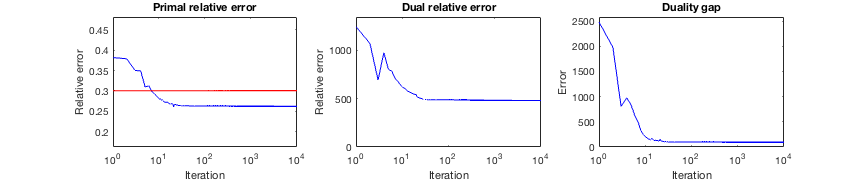
\includegraphics[scale=0.6]{noisy_random_signal_relative_errors_stagnate}
\caption{Primal relative error (\ref{Eqn:term_crit-candidate_residuals}d), dual relative error (\ref{Eqn:term_crit-candidate_residuals}b), and duality gap (\ref{Eqn:term_crit-candidate_residuals}f) for 10,000 iterates of the GDD algorithm (Algorithm \ref{Alg:PGD}) applied to a natural noise model with $n=16$, $L=6$ observations, and noise ratio $0.30$.  The horizontal axis is log-plotted to highlight early progress along with later stagnation.  The pair $(X_\star, y_\star)$ are computed with \texttt{SDPT3}.}
\label{Fig:noisy_random_relative_errors_stagnate}
\end{figure}
% experiments.figure.noisyrandom_relative_errors_stagnate


Figure \ref{Fig:noisy_random_relative_errors_stagnate} demonstrates that the GDD algorithm stagnates when attempting to solve a PLGD model with Gaussian noise (\ref{Eqn:PhaseLift-GD_Gaussian_noise}).  In this problem, primal feasibility (\ref{Eqn:saga_conv_crit_primal}) is acheived at iterate 6, and further progress is made over the following early iterations, as indicated by the primal relative error (\ref{Eqn:term_crit-candidate_residuals}d) plot.  However, the strong duality condition (\ref{Eqn:saga_conv_crit_gap}) is never satisfied, and the final duality gap at iterate 10,000 is 97.63.  Likewise, the dual variable $y_k$ does not approach the optimal dual variable $y_\star$, as indicated by the dual relative error (\ref{Eqn:term_crit-candidate_residuals}b) plot.  In this particular PLGD model, $X_\star$ is rank three, causing the dual objective $\lambda_1(\caA^*y)$ to be nondifferentiable near $y_\star$ per Corollary \ref{Cor:PLGD-optimality} (e).  Thus the GDD algorithm identifies the dual objective $\lambda_1(\caA^*y)$ as nondifferentiable at iterate 84 reverts to the monotone stepsize sequence (\ref{Eqn:GD-steplength}).  


The next experiment establishes that PLGD models with Gaussian noise (\ref{Eqn:PhaseLift-GD_Gaussian_noise}) almost always have an optimal matrix $X_\star$ with rank greater than one, and this rank problem causes the stagnation of the GDD algorithm.  Table \ref{Tab:average_rank_soln_matrix_with_gaussian_dual_variable} compares PLGD models with synthetic (\ref{Eqn:PhaseLift-GD_synthetic_noise}) and Gaussian noise (\ref{Eqn:PhaseLift-GD_Gaussian_noise}), depicting the rank of the optimal matrix $X_\star$ and the behavior of the GDD algorithm.

\begin{table}[H]
\centering 
\begin{tabular}{ |cc|c|c|c|c|c|c| }
\hline
	\multicolumn{2}{|c|}{} &	\multicolumn{3}{c|}{Synthetic noise} 	&	\multicolumn{3}{c|}{Gaussian noise}  \\
\multicolumn{2}{|c|}{}  	&	\multicolumn{1}{c}{$L = 4$}	&	\multicolumn{1}{c}{$L = 6$}	&	\multicolumn{1}{c|}{$L = 8$} &	\multicolumn{1}{c}{$L = 4$}	&	\multicolumn{1}{c}{$L = 6$}	&	\multicolumn{1}{c|}{$L = 8$}		\\
\hline
& $\textnormal{rank}(X_\star)$
	&	1	&	1	&	1	&	3.41 	&	3.28 	&	3.27 \\
$\epsilon_\rel = 0.05$ &	 GDD itns.
	&	125.09	&	144.20 & 182.26	&	1,000	&	1,000	&	1,000\\
& 	duGap
	&	$1.17_{-4}$  &  $1.18_{-4}$ &  $1.18_{-4}$ 	&	9.60   & 3.88   & 3.86\\
\hline
& $\textnormal{rank}(X_\star)$
	&	1	&	1	&	1	&	2.99 	&	3.00 &	3.04 \\
$\epsilon_\rel = 0.15$ &	 GDD itns.
	&	62.48  & 85.32 &  95.58	&	1,000	&	1,000	&	1,000\\
& 	duGap
	&	$1.20_{-4}$ &  $1.35_{-4}$ &  $1.33_{-4}$ &	15.9 &  14.0 &  15.8 \\
\hline
& $\textnormal{rank}(X_\star)$
	&	1	&	1	&	1	&	2.64  	&	2.70  &	2.89\\
$\epsilon_\rel = 0.30$ &	 GDD itns.
	&	40.34  & 50.88  & 64.28	&	1,000	&	1,000	&	1,000\\
& 	duGap
	&	$1.17_{-4}$ &  $1.23_{-4}$ &  $1.27_{-4}$		&	   21.2 &  26.7  & 31.5\\
 \hline
\end{tabular}
\vspace{0.5cm}
\caption{The GDD algorithm (Algorithm \ref{Alg:PGD}) results and optimal matrix rank for PLGD models with synthetic (\ref{Eqn:PhaseLift-GD_synthetic_noise}) and Gaussian noise (\ref{Eqn:PhaseLift-GD_Gaussian_noise}).  This table depicts the mean rank of $X_\star$, number of the GDD algorithm iterations, and final duality gap (\ref{Eqn:term_crit-candidate_residuals}f) (duGap) for 100 random phase retrieval models with signal size $n=16$, noise ratio $\epsilon_\rel$, and oversampling $L$.  In all synthetic noise models (\ref{Eqn:PhaseLift-GD_synthetic_noise}), the solution $X_\star$ was rank-one and the GDD algorithm converged.  In all Gaussian noise models (\ref{Eqn:PhaseLift-GD_Gaussian_noise}), the algorithm reached the maximum of 1,000 iterations without attaining the termination condition (\ref{Eqn:saga_conv_crit_gap}).  Note that pairs $(X_\star, y_\star)$ are computed with \texttt{SDPT3} and numbers $n_{-k}$ are shorthand for $n \times 10^{-k}$.} \label{Tab:average_rank_soln_matrix_with_gaussian_dual_variable}
\end{table}
% experiments.table.noisyrandom_mean_rank_lifted_signal_exact_solution


Table \ref{Tab:average_rank_soln_matrix_with_gaussian_dual_variable} demonstrates that PLGD models with Gaussian noise (\ref{Eqn:PhaseLift-GD_Gaussian_noise}) typically have optimal matrices with rank greater than one, causing the GDD algorithm to stagnate.  
The GDD algorithm cannot attain an optimal primal matrix $X_\star$ with rank greater than one because the primal recovery (\ref{Eqn:GD-primal_rec2}) and refinement (\ref{Eqn:GD-PFD}) steps used in this algorithm only return a rank-one matrix $X = xx^*$.  
Additionally, Corollary \ref{Cor:PLGD-optimality}, (e) indicates that $\text{rank}(X_\star)$ is a lower bound on the multiplicity of the algebraically largest eigenvalue of $\caA^*y_\star$.  
Thus the objective function $\lambda_1(\caA^*y)$ will be nondifferentiable in some neighborhood around $y_\star$ and the GDD algorithm will stagnate prior to approaching $y_\star$.  
As a result, the GDD algorithm cannot attain a pair $(X,y)$ that are sufficiently close to the optimal pair $(X_\star, y_\star)$ and fails to satisfy the duality gap condition (\ref{Eqn:saga_conv_crit_gap}).


In contrast to the Gaussian models (\ref{Eqn:PhaseLift-GD_Gaussian_noise}), we see that PLGD models with synthetic noise (\ref{Eqn:PhaseLift-GD_synthetic_noise}) consistenly have rank-one optimal matrices $X_\star$, allowing the GDD algorithm to converge.  
Each synthetic noise model (\ref{Eqn:PhaseLift-GD_synthetic_noise}) in Table \ref{Tab:average_rank_soln_matrix_with_gaussian_dual_variable} had an optimal dual matrix $\caA^*y_\star$ with a unique algebraically largest eigenvalue, making the dual objective function $\lambda_1(\caA^*y)$ differentiable at $y_\star$ and allowing the GDD algorithm to approach the optimal dual variable $y_\star$.  
Once the pair $(X,y)$ are sufficiently close to the optimal pair, the duality gap condition (\ref{Eqn:saga_conv_crit_gap}) is met and convergence is declared.
At this point, the primal recovery equation (\ref{Eqn:PLGD-noise_is_dual_variable}) successfully denoises the noisy observation $b = \mathbf{b} + \epsilon y_\star / ||y_\star||_2$ because the synthetic noise steps (\ref{Def:synthetic_noise}) guarantee an exact relation $\eta = \epsilon y_\star / ||y_\star||_2$ between the noise term $\eta$ and optimal dual variable $y_\star$.
Thus the GDD algorithm is able to return a matrix $X$ which accurately approximates the optimal matrix $X_\star = \mathbf{x}\mathbf{x}^*$.  










Table \ref{Tab:average_rank_soln_matrix_with_gaussian_dual_variable} also helps to explain why dual refinement (Algorithm \ref{Alg:PGD}, step 13) is not beneficial for PLGD models with Gaussian noise (\ref{Eqn:PhaseLift-GD_Gaussian_noise}).  As we saw in Table \ref{Tab:noiseless_runtimes}, an inaccurate signal $x$ can cause the dual refinement problem (\ref{Eqn:GD-DFP}) to return an unreliable update $\hat{y}$.  Figure \ref{Fig:noisy_random_DFP_vs_no_DFP} depicts the progress made by the GDD algorithm with and without dual refinement for three PLGD models with Gaussian noise (\ref{Eqn:PhaseLift-GD_Gaussian_noise}).

\begin{figure}[H]
\hbox{\hspace{-1.0cm}  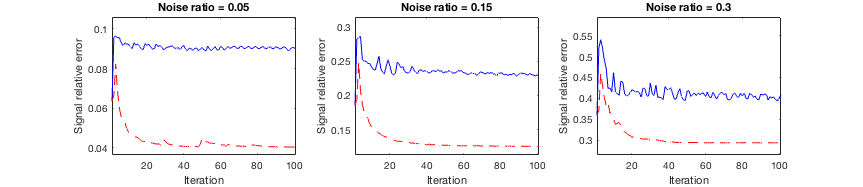
\includegraphics[scale=0.6]{noisy_random_signal_DFP_vs_no_DFP}}
\caption{A comparison of the GDD algorithm (Algorithm \ref{Alg:PGD}) with and without dual refinement (\ref{Eqn:GD-DFP}) for PLGD models with Gaussian noise (\ref{Eqn:PhaseLift-GD_Gaussian_noise}) with various noise levels, with random Gaussian signal of size $n = 128$ and $L = 10$ observations.  The solid blue line indicates dual refinement, and the dashed red line indicates no dual refinement.}
\label{Fig:noisy_random_DFP_vs_no_DFP}
\end{figure}
% experiments.figure.noisyrandom_dual_refinement_fails



Figure \ref{Fig:noisy_random_DFP_vs_no_DFP} demonstrates that the dual refinement step (\ref{Eqn:GD-DFP})  inhibits the progress otherwise made by the GDD algorithm.  This step is initialized with a signal $x$ which corresponds to the rank-one matrix iterate $X = xx^*$.  Since the optimal matrix $X_\star$ tends to have rank greater than one, the dual refinement problem (\ref{Eqn:GD-DFP}) will not be properly initialized and may return a poor update $\hat{y}$.  Thus the dual refinement step in the GDD algorithm is not beneficial for signal recovery in phase retrieval problems with Gaussian noise (\ref{Eqn:phase_retrieval_Gaussian_noise}).





\section{New Termination Conditions}  	\label{Subsec:PLGD_term_crit-new_term_crit}


In Section \ref{Subsec:PLGD_term_crit-stagnation}, we saw that the GDD algorithm (Algorithm \ref{Alg:PGD}) tends to stagnate when solving phase retrieval problems with Gaussian noise (\ref{Eqn:phase_retrieval_Gaussian_noise}), failing to satisfy the duality gap termination condition (\ref{Eqn:saga_conv_crit_gap}) original established in \cite{DBLP:journals/siamsc/FriedlanderM16}.  
This section establishes new termination conditions for the GDD algorithm for PLGD models with Gaussian noise (\ref{Eqn:PhaseLift-GD_Gaussian_noise}) and demonstrates the effectiveness of these conditions for identifying stagnation of the GDD algorithm.  
(For a comparison of the unused residuals from (\ref{Eqn:term_crit-candidate_residuals}), see Appendix \ref{Sec:Appx-further_reasons_for_new_term_crit}.)







We begin by presenting the new termination conditions for the GDD algorithm for PLGD models with Gaussian noise (\ref{Eqn:PhaseLift-GD_Gaussian_noise}).  To identify stagnation of the GDD algorithm and declare termination, the primal difference (\ref{Eqn:term_crit-candidate_residuals}e) is set to 
\begin{equation}
	\label{Eqn:term_crit_new-primal_difference}
\frac{| \rho - \hat{\rho} |}{\rho} \leq  \textnormal{tol}_\textnormal{primal} = 10^{-5}, \ \ \rho = ||\caA(xx^*) - b||_2
\end{equation}
and the dual variable difference (\ref{Eqn:term_crit-candidate_residuals}i) is set to
\begin{equation}
	\label{Eqn:term_crit_new-dual_difference}
\frac{||y- \hat{y}||_2}{||y||_2} \leq \textnormal{tol}_\textnormal{dual}= 10^{-4},
\end{equation}
where a hat indicates the previous iterate (e.g., $\hat{y} = y_{k-1}$).  Termination is declared when (\ref{Eqn:term_crit_new-primal_difference}) and (\ref{Eqn:term_crit_new-dual_difference}) are satisfied or after a maximum of 300 iterations are performed.  After termination, the signal returned corresponds to the signal among the previous 20 with the smallest duality gap (\ref{Eqn:term_crit-candidate_residuals}f) value.  










To demonstrate the effectiveness of these termination conditions, we consider a set of six PLGD models with Gaussian noise (\ref{Eqn:PhaseLift-GD_Gaussian_noise}) solved with the GDD algorithm.   The signal relative error (\ref{Eqn:term_crit-candidate_residuals}a) serves as a control measurement to identify when the GDD algorithm has stagnated and should terminate.  Figure \ref{Fig:term_crit-signal_err} depicts the signal relative error (\ref{Eqn:term_crit-candidate_residuals}a) for each of these models.


\newpage

\begin{figure}[H]
\centering
\hbox{\hspace{-1.2cm} 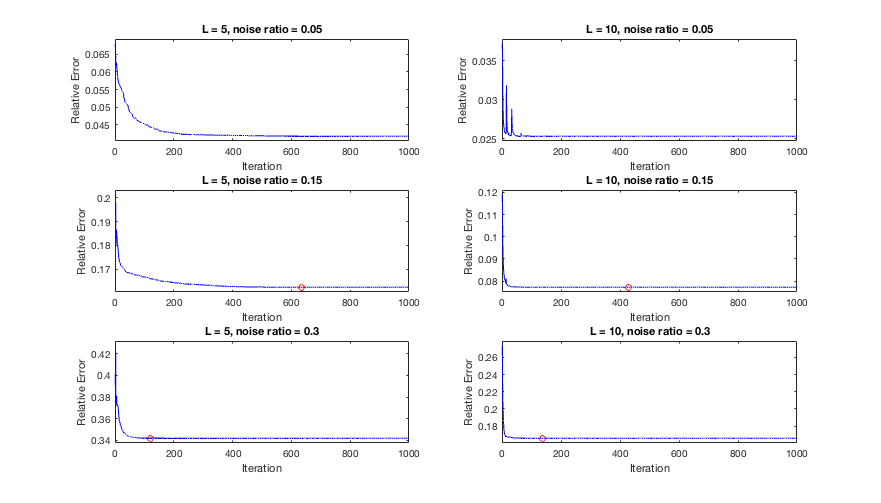
\includegraphics[scale=0.6]{term_crit-signal_err} }\vspace{-0.4cm}
\caption{Signal relative errors (\ref{Eqn:term_crit-candidate_residuals}a) for six PLGD models with Gaussian noise (\ref{Eqn:PhaseLift-GD_Gaussian_noise})  solved with the GDD algorithm (Algorithm \ref{Alg:PGD}). The image in Figure \ref{Fig:parrot_signal_iterates} was resized to $64 \times 64$ pixels, made grayscale, and six models were generated with oversampling rates of $L = 5, 10$ and noise ratios $\epsilon_\rel = 0.05, 0.15, 0.30$.  These models were then solved using the GDD algorithm set to terminate after 1,000 iterations.  The red circle (where present) indicates when the dual objective was determined nondifferentiable.}
\label{Fig:term_crit-signal_err}
\end{figure}
% experiments.figure.noisyimage_new_termination_criteria

Figure \ref{Fig:term_crit-signal_err} depicts the early progress and quick stagnation of the GDD algorithm for these PLGD models with Gaussian noise (\ref{Eqn:PhaseLift-GD_Gaussian_noise}).  For each model, virtually no measurable progress was made after iteration 500.  Yet the point at which each model stagnates appears to differ, and in one case ($L = 10$ and $\epsilon_\rel = 0.05$) the signal quality appears to vary greatly for neighboring iterates.  Thus we examine the behavior in Figure \ref{Fig:term_crit-signal_err} to identify the desired interval of iterates in which the GDD algorithm should terminate for each model.




The results in Figure \ref{Fig:term_crit-signal_err} suggest that models with a larger oversampling rate and those with a larger noise ratio make progress faster and stagnate earlier.  One indicator that the point of stagnation differs for these models is the point at which the GDD algorithm identifies the objective function $\lambda_1(\caA^*y)$ as nondifferentiable (i.e., the condition (\ref{Eqn:GD-diff_tol}) fails).  The models in Figure \ref{Fig:term_crit-signal_err} with the least noise never identified a nondifferentiable objective, whereas the noisiest models identified nondifferentiable objectives very early (at iterate 122 for $L=5$ and 137 for $L=10$).  Another indicator that the models of Figure \ref{Alg:PGD} stagnate at different rates is the point at which the primal objective is found to be feasible, as described in Table \ref{Tab:term_crit-pr_feas_faster_for_big_L_noise}.

\begin{table}[H]
\centering
\begin{tabular}{ |c|c|c| }
\hline
&	$L = 5$
	&	$L = 10$	\\
 \hline
$\epsilon_\rel = 0.05$
&     33 &   3 		\\
 \hline
$\epsilon_\rel = 0.15$
&  N/A &  3 	\\
 \hline
$\epsilon_\rel = 0.30$
&  22 &  3	\\
 \hline
\end{tabular}
\vspace{0.5cm}
\caption{Iterate at which the GDD algorithm (Algorithm \ref{Alg:PGD}) became primal feasible for models from Figure \ref{Fig:term_crit-signal_err}.}
	\label{Tab:term_crit-pr_feas_faster_for_big_L_noise}
\end{table}
% experiments.figure.noisyimage_new_termination_criteria

Table \ref{Tab:term_crit-pr_feas_faster_for_big_L_noise} shows that all three models with oversampling $L = 10$ found feasible signals after just 3 iterations, yet the models with $L = 5$ were a bit slower, and in particular the model with $L = 5$ and $\epsilon_\rel = 0.15$ never identified a feasible signal.


Based on these observations, Table \ref{Tab:term_crit-desired_termination_windows} proposes iterate intervals in which the GDD algorithm appears to have stagnated for each model in Figure \ref{Fig:term_crit-signal_err}, providing a guideline for assessing the new termination conditions (\ref{Eqn:term_crit_new-primal_difference}) and (\ref{Eqn:term_crit_new-dual_difference}).
\begin{table}[H]
\centering
\begin{tabular}{ |c|c|c| }
\hline
&	$L = 5$
	&	$L = 10$	\\
 \hline
$\epsilon_\rel = 0.05$
&     200-400 &   50-200 		\\
 \hline
$\epsilon_\rel = 0.15$
&  200-400 &  50-100 	\\
 \hline
$\epsilon_\rel = 0.30$
&  100-200 &  50-100	\\
 \hline
\end{tabular}
\vspace{0.5cm}
\caption{Intervals of iterates at which the GDD algorithm (Algorithm \ref{Alg:PGD}) appears to stagnate for models from Figure \ref{Fig:term_crit-signal_err}.}
	\label{Tab:term_crit-desired_termination_windows}
\end{table}







In order to demonstrate that the primal difference (\ref{Eqn:term_crit-candidate_residuals}e) and dual variable difference (\ref{Eqn:term_crit-candidate_residuals}i) are accurate indicators of the stagnation of the GDD algorithm, Figure \ref{Fig:term_crit-pr_and_dual} depicts the behavior of these residuals for the models in Figure \ref{Fig:term_crit-signal_err}.  
Note that the vertical axis indicates specific tolerances and the horizontal axis indicates the first iterate at which the GDD algorithm would satisfy this tolerance.


\begin{figure}[H]
\centering
\hbox{\hspace{-1.4cm} 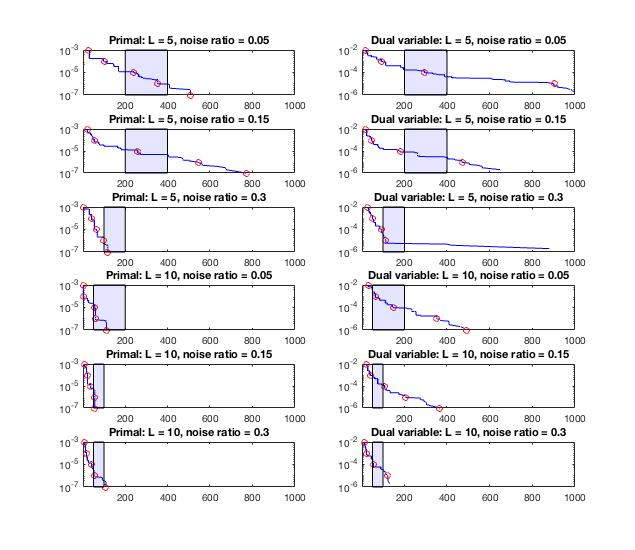
\includegraphics[scale=0.6]{term_crit-pr_and_dual} }\vspace{-1.3cm}
\caption{Plots of tolerance values against the iterate at which the GDD algorithm (Algorithm \ref{Alg:PGD}) first satisfies this tolerance for the models discussed in Figure \ref{Fig:term_crit-signal_err}.  Tolerances depicted are difference values for the primal objective (\ref{Eqn:term_crit-candidate_residuals}e) and dual variable (\ref{Eqn:term_crit-candidate_residuals}i).  Red circles are placed at tolerances $10^{-n}$.  The blue rectangles indicate the proposed intervals of termination from Table \ref{Tab:term_crit-desired_termination_windows}.}
\label{Fig:term_crit-pr_and_dual}
\end{figure}
% experiments.figure.noisyimage_new_termination_criteria



For each of the models in Figure \ref{Fig:term_crit-pr_and_dual}, the termination conditions (\ref{Eqn:term_crit_new-primal_difference}) and (\ref{Eqn:term_crit_new-dual_difference}) are satisfied within or close to each respective interval of stagnation from Table \ref{Tab:term_crit-desired_termination_windows}.  For the models with oversampling $L = 5$, the GDD algorithm satisfies the tolerances $\tol_\textnormal{primal} = 10^{-5}$ from (\ref{Eqn:term_crit_new-primal_difference}) and $\tol_\textnormal{dual} = 10^{-4}$ from (\ref{Eqn:term_crit_new-dual_difference}) within or slightly prior to each respective desired interval.  Likewise, the GDD algorithm achieve these desired tolerances for the models with $L =10$ within or slightly after each desired interval.  As an additional precaution, the maximum iteration count of 300 iterates will prevent running the GDD algorithm after it has stagnated.

Note that there is also theoretical justification for selecting the dual variable difference (\ref{Eqn:term_crit-candidate_residuals}i) as a termination condition.  Proposition \ref{Prop:PLGD-opt_unconstrained} showed that the variable $y$ is optimal for the PLGD model (\ref{Eqn:PhaseLift-P-GD}) if $y = \Pi_\caC(y - \alpha g)$ for some $g \in \partial f(y)$ and all $\alpha > 0$.  This property corresponds to the termination condition 
\begin{equation*}
|| \Pi_\caC(y - \alpha g) - y ||_2 \leq \text{tol}.
\end{equation*}
If we make this condition relative by setting $\text{tol} = 10^{-4}||\Pi_\caC(y - \alpha g)||_2$, then we recover the new dual variable difference condition (\ref{Eqn:term_crit_new-dual_difference}).






One additional concern for termination conditions is the nonmonotonic nature of the GDD algorithm.  In Figure \ref{Fig:term_crit-signal_err}, the model with $L = 10$ and $\epsilon_\rel = 0.05$ demonstrates that the GDD algorithm may produce neighboring signal iterates with varying accuracy.  Since this algorithm is nonmonotonic and relies on a subroutine to recover the current approximate signal, the accuracy of the sequence of recovered signals can vary dramatically.  Thus we need a reliable indicator to select a sufficiently accurate signal among the previous iterates.  Figure \ref{Fig:term_crit-duality_gap} depicts the signal relative error (\ref{Eqn:term_crit-candidate_residuals}a) and duality gap (\ref{Eqn:term_crit-candidate_residuals}f) for the $L = 10$, $\epsilon_\rel = 0.05$ model.  Note that the new termination conditions $\tol_\text{primal} = 10^{-5}$ and $\tol_\text{dual} = 10^{-4}$ would select the 148th iterate as the candidate solution.  



\begin{figure}[H]
\centering
\hbox{\hspace{-1.7cm} 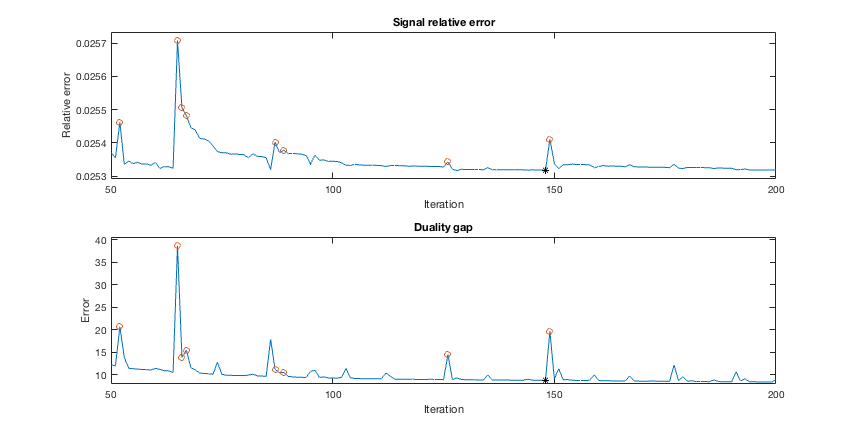
\includegraphics[scale=0.6]{term_crit-duality_gap} }
\caption{Signal relative error (\ref{Eqn:term_crit-candidate_residuals}a) and duality gap (\ref{Eqn:term_crit-candidate_residuals}f) for the model from Figure \ref{Fig:term_crit-signal_err} with oversampling $L = 10$ and noise ratio $\epsilon_\rel = 0.05$. Red circles indicate signals with relative error at least $0.05\%$ above the mean of their ten neighbors, and the black asterisk indicates both the final iterate based on new termination conditions and the optimal iterate based on minimum duality gap.}
\label{Fig:term_crit-duality_gap}
\end{figure}

% experiments.figure.noisyimage_new_termination_criteria



Figure \ref{Fig:term_crit-duality_gap} demonstrates that the duality gap (\ref{Eqn:term_crit-candidate_residuals}f) violation closely matches the signal relative error (\ref{Eqn:term_crit-candidate_residuals}a).  Among the previous iterates, those with the least accurate signal (indicated by the red circle) are accurately identified as having a duality gap value greater than the minimum (black asterisk).  Thus once the GDD algorithm terminates, we select the signal among the last 20 with the lowest duality gap value.








Given the new termination conditions (\ref{Eqn:term_crit_new-primal_difference}), (\ref{Eqn:term_crit_new-dual_difference}), the maximum iteration count of 300, and the signal selection method discussed above, the Figure \ref{Fig:term_crit-model_term_for_tols} depicts the iterate at which the GDD algorithm would terminate for each PLGD model with Gaussian noise from Figure \ref{Fig:term_crit-signal_err}.

\begin{figure}[H]
\centering
\hbox{\hspace{-1.9cm} 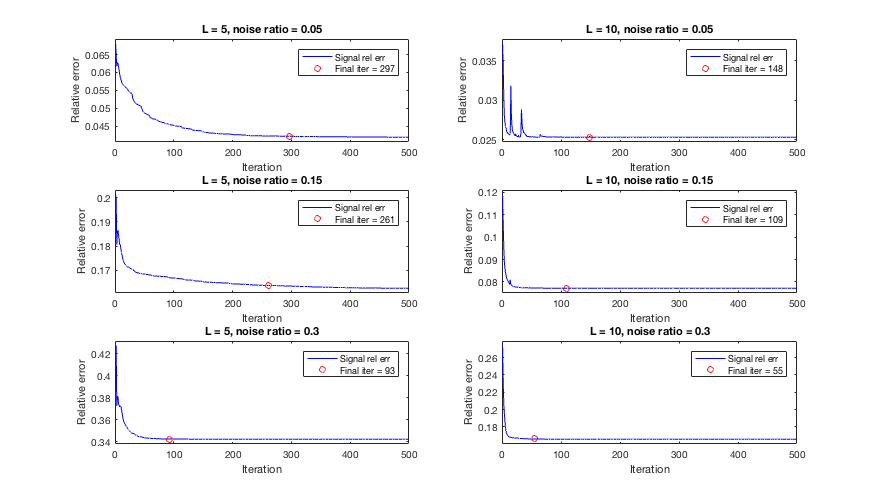
\includegraphics[scale=0.6]{term_crit-model_term_for_tols} }\vspace{-0.4cm}
	\caption{Iterate at which the GDD algorithm (Algorithm \ref{Alg:PGD}) terminates for the models from Figure \ref{Fig:term_crit-signal_err} based on new termination conditions.}
\label{Fig:term_crit-model_term_for_tols}
\end{figure}
% experiments.figure.noisyimage_new_termination_criteria

For each model in Figure \ref{Fig:term_crit-model_term_for_tols}, the GDD algorithm successfully terminates within or nearby the interval of stagnation established in Table \ref{Tab:term_crit-desired_termination_windows}.
Given the new termination conditions (\ref{Eqn:term_crit_new-primal_difference}) and (\ref{Eqn:term_crit_new-dual_difference}), we may now treat the GDD algorithm as a black-box algorithm for noisy phase retrieval and examine the sequence of eigenvalue problems generated by the GDD algorithm.





\newpage



\chapter{Eigenvalue Computation}		\label{Sec:evol_mats}



\section{Introduction}   \label{Subsec:evol_mats-intro}


In this chapter we examine the \textit{evolving matrix eigenvalue problem} (EMEP) in Algorithm \ref{Alg:PGD} and develop a new strategy for solving this problem.


Section \ref{Subsec:evol_mats-spectral_props} defines the EMEP and examines its computational costs and evolving spectrum across matrix iterates $A_k$.  
In particular, we observe that the algebraically largest eigenvalues tend to cluster as the algorithm proceeds, leading to more difficult eigenvalue problems for later matrix iterates.  
To handle these eigenvalue problems, Section \ref{Subsec:evol_mats-IRAM} reviews the \textit{implicitly restarted Arnoldi method} (IRAM) \cite{sorensen1992implicit}, a modern Krylov subspace method. 
The convergence behavior of the IRAM is based on the spectrum of the given eigenvalue problem as well as the IRAM parameters chosen by the user.
To understand and exploit the convergence behavior of the IRAM, Section \ref{Subsec:evol_mats-IRAM} reviews the subroutines of the IRAM and summarizes relevant convergence results.


Next, Section \ref{Subsec:evol_mats-adaptive_IRAM} presents \textit{the IRAM with adaptive parameter selection}, a new strategy for solving the EMEP by adaptively changing
the number of requested eigenvalues $r$ in the IRAM (Algorithm \ref{Alg:IRAM}).
Section \ref{Subsec:evol_mats-correl_btwn_EMEP_and_IRAM} closely examines the EMEP for two PLGD models with Gaussian noise (\ref{Eqn:PhaseLift-GD_Gaussian_noise}) to demonstrate an observed correlation between the clustering of the algebraically largest eigenvalues in the EMEP and an increase in the optimal choice of parameter $r$ in the IRAM.
We see that the IRAM with adaptive parameter selection properly tracks the optimal choice of $r$ for these models.
Performance results for the IRAM with adaptive parameter selection are presented in  Chapter \ref{Sec:Numerics}.
Also note that all \emep \ experiments in this chapter are performed with Algorithm \ref{Alg:PGD} using the new termination conditions (\ref{Eqn:term_crit_new-primal_difference}) and (\ref{Eqn:term_crit_new-dual_difference}) established in Chapter \ref{Sec:PLGD_term_crit} and are available for reproduction.\footnote{\url{https://github.com/Will-Wright/low-rank-opt-rapid-eig}}




\section{The Evolving Matrix Eigenvalue Problem}		\label{Subsec:evol_mats-spectral_props}


In this section we examine the sequence of eigenvalue problems in Algorithm \ref{Alg:PGD}, which we define as the \textit{evolving matrix eigenvalue problem} (EMEP).
We will see that the EMEP is the most computationally expensive subroutine in Algorithm \ref{Alg:PGD}.  
We also observe that the EMEP matrix iterates have a spectrum which evolves in a predictable way from early to later iterates.




\subsection{EMEP Definition} 	\label{Subsubsec:evol_mats-EMEP_definition}


We begin by formally defining the EMEP.
Generally speaking, we are concerned with a sequence of eigenvalue problems in which each eigenvalue problem is dependent on the results of the previous problem.  
For each iterate $k$ in this sequence of problems, we have some Hermitian matrix iterate $A_k \in \caH^n$ and seek its $j$ algebraically largest eigenvalues $\Lambda^{(k)}_j$ and the corresponding eigenvectors $V^{(k)}_j$.  
%Next, the previous set of basis matrices $\caV_{k} = \{ V^{(i)}_j \}_{i=0}^{k}$ are used to find the next matrix iterate $A_{k+1}$.  
%More specifically, we are concerned with problems of the form
%\begin{equation} 		\label{Eqn:EMEP_general}
%\begin{array}{ll}
%\textnormal{for}
%	&	k = 1, 2, \ldots, K		\\
%\textnormal{find}	
%	&	\left( \Lambda^{(k)}_j, \ V^{(k)}_j \right) \textnormal{ of } A_k
%\end{array}
%\end{equation}
%where $\Lambda^{(k)}$ are the $j$ algebraically largest eigenvalues of $A_k$, $V_k$ is the matrix of corresponding eigenvectors, $A_k \in \caH^n$ is dependent on $\caV_{k} = \{ V^{(i)}_j \}_{i=0}^{k}$, and $V_0 \in \bbC^{n \times j}$ is an initial basis matrix.
Some examples of this problem include subspace tracking in signal processing (see, e.g., \cite{comon1990tracking}, \cite{stewart1992updating}, \cite{yang1995projection}, \cite{doukopoulos2008fast}), matrix completion (e.g., \cite{ngo2012scaled}), and the Kohn-Sham equation in density functional theory (e.g., \cite{saad2010numerical}).



%To see that each eigenvalue problem in Algorithm \ref{Alg:PGD} is dependent on the results of the previous eigenvalue problems, 

%(Also note that the iterate $k$ does not correspond to the iterate number in Algorithm \ref{Alg:PGD} because step 6 involves a linesearch which may involve more than one eigenvalue problem.)  

%We will show that each matrix iterate $A_k = \caA^*y_k$ in Algorithm \ref{Alg:PGD} is computed using a variable $y_k$ which is dependent on the previous set of basis vectors $\caV_{k-1} = \{ v_1^{(i)} \}_{i=0}^{k-1}$.  

%It can be shown inductively that $y_k$ is a function of $\caV_{k-1}$.  The initial iterate $k = 0$ corresponds to the first eigenvalue problem in Algorithm \ref{Alg:PGD}, where $y_0 = \Pi_\caC(b)$ is initialized using the observation vector $b$ and is independent of any eigenvector.  



To define the EMEP, first note that each eigenvalue problem in Algorithm \ref{Alg:PGD} (steps 2, 6, and 14) requires the two algebraically largest eigenvalues of the matrix iterate $A_k = \caA^*y_k$, where $\caA^*$ is defined as (\ref{Eqn:A_definition_with_masks}).
In Algorithm \ref{Alg:PGD}, the matrix $A_0$ is initialized as $A_0 = \caA^*b$, where $b$ is the observation vector in the PLGD model (\ref{Eqn:PhaseLift-P-GD}).
For each iterate $k >0$, the update matrix $A_k = \caA^*y_k$ is computed with $y_k = \Pi_{\caC}(y_{k-1}- \alpha_{k-1}  g_{k-1})$, where the gradient $g_{k-1} = \caA(v_{k-1} v_{k-1}^*)$ is a function of $v_{k-1}$ and the steplength $\alpha_{k-1}$ is determined using a linesearch on the minimization problem
\begin{equation}			\label{Eqn:EMEP_linesearch_prob_in_evol_mats_chapter}
\begin{array}{ll}
\min\limits_{\substack{\alpha}}
	&	\lambda_1 \left( \caA^* ( \Pi_\caC ( y_{k-1} - \alpha g_{k-1} ) )  \right).
\end{array}
\end{equation}
Thus we define the sequence of eigenvalue problems generated by Algorithm \ref{Alg:PGD} as the \textit{evolving matrix eigenvalue problem} (EMEP)
\begin{equation}		\label{Eqn:EMEP_PLGD}
\begin{array}{ll}
\textnormal{for}
	&	k = 1, 2, \ldots, K		\\
\textnormal{find}	
	&	\left( \lambda^{(k)}_1, \ v^{(k)}_1 \right) \textnormal{ and } \left( \lambda^{(k)}_2, \ v^{(k)}_2 \right) \textnormal{ of } A_k,
\end{array}
\end{equation}
where $\lambda^{(k)}_1$ and $\lambda^{(k)}_2$ are the two algebraically largest eigenvalues of the \textit{matrix iterate} $A_k = \caA^*y_k$, and $y_k$ is the previous dual variable generated by Algorithm \ref{Alg:PGD} (from step 2, 6, or 14).
Note that $y_k$ is dependent on $v_{k-1}$ and $y_{k-1}$, and thus each eigenvalue problem in Algorithm \ref{Alg:PGD} is dependent on the previous matrix iterate $A_{k-1}$.
Also note that the steplength $\alpha_{k-1}$ returned by the linesearch problem (\ref{Eqn:EMEP_linesearch_prob_in_evol_mats_chapter}) influences the rate at which the sequence of matrices $A_0, A_1, \ldots$ evolves, since
\begin{equation}
\begin{split}
||A_k - A_{k-1}||
	& = ||\caA^* ( \Pi_\caC ( y_{k-1} - \alpha_{k-1} g_{k-1})) - \caA^*y_{k-1} ||		\\
	& = ||\caA^* ( \Pi_\caC ( y_{k-1} - \alpha_{k-1} g_{k-1}) - y_{k-1}) ||		\\
	& \leq ||\caA^*|| \cdot || \Pi_\caC ( y_{k-1} - \alpha_{k-1} g_{k-1}) - y_{k-1} ||	 	\\
	& \leq ||\caA^*|| \cdot || y_{k-1} - \alpha_{k-1} g_{k-1} - y_{k-1} || 
		= ||\caA^*|| \cdot |\alpha_{k-1}| \cdot	||g_{k-1}||.	\\
\end{split}
\end{equation}




\subsection{Computational Costs} 	\label{Subsubsec:evol_mats-EMEP_compu_costs}


Next, we examine the overall computational costs of the \emep.
As discussed in Section \ref{Subsec:PLGD_algo-algo}, the main computational costs in Algorithm \ref{Alg:PGD} are the EMEP (step 2, 6, and 14), the primal refinement (step 11), and the dual refinement (step 13).  
Since we are focused on PLGD models with Gaussian noise (\ref{Eqn:PhaseLift-GD_Gaussian_noise}), the dual refinement step of Algorithm \ref{Alg:PGD} is skipped (see the end of Section \ref{Subsec:PLGD_term_crit-stagnation} for an explanation).
In both the \emep \ and the primal refinement step, the primary computational cost comes from $\caA$-products (\ref{Eqn:A_definition_with_masks}), where each $\caA(xx^*)$ product requires $L$ DFTs and each $[\caA^*y]x$ product requires $2L$ DFTs.  
Thus we measure computational costs in terms of the number of DFTs, following the convention of \cite{DBLP:journals/tit/CandesLS15} and \cite{DBLP:journals/siamsc/FriedlanderM16}.
Also note that the computation of the eigenpair $(\lambda_1, v_1)$ in the \emep \ must be very accurate in order to determine an accurate descent step $g = \caA(v_1v_1^*)$ in Algorithm \ref{Alg:PGD}.
Table \ref{Tab:EMEP_costs} depicts the number of DFTs in Algorithm \ref{Alg:PGD} for a variety of noisy problems.
\begin{table}[H]
\centering
\begin{footnotesize}
\hbox{

\hspace{0.25cm}
\begin{tabular}{ |ccc|ccc|cc|cc| }
 \hline
			&&&  \multicolumn{3}{c|}{EMEP} 
			&  \multicolumn{2}{c|}{Primal refinement}
			& 	\multicolumn{2}{c|}{All other steps}	\\
$n$ & $L$ & $\epsilon_\text{rel}$ 	& \texttt{eigs} calls  & Minutes & DFTs & Minutes  & DFTs & Minutes  & DFTs   \\
 \hline
 4,096 &  5 & 0.05 & 228 & 13.13  (0.94) &  51,935  (0.97) & 0.73  (0.05) &   1,516  (0.03) & 0.04 &     17 	\\
 4,096 &  5 & 0.15 & 120 & 6.63  (0.94) &  31,085  (0.97) & 0.45  (0.06) &   1,076  (0.03) & 0.01 &     10 \\
 4,096 &  5 & 0.30 &  52 & 3.56  (0.89) &  16,410  (0.95) & 0.45  (0.11) &    854  (0.05) & 0.01 &      4 \\
 4,096 & 10 & 0.05 & 190 & 12.06  (0.96) &  72,587  (0.98) & 0.45  (0.04) &   1,819  (0.02) & 0.03 &     29	\\ 
 4,096 & 10 & 0.15 & 106 & 8.60  (0.96) &  51,450  (0.98) & 0.30  (0.03) &   1,194  (0.02) & 0.02 &     17 \\
 4,096 & 10 & 0.30 & 111 & 17.95  (0.98) & 107,936  (0.99) & 0.36  (0.02) &   1,420  (0.01) & 0.01 &     18 \\
 \hline
16,384 &  5 & 0.05 & 199 & 46.09  (0.95) &  69,745  (0.98) & 2.13  (0.04) &   1,468  (0.02) & 0.06 &     16	\\
16,384 &  5 & 0.15 &  91 & 27.71  (0.95) &  41,880  (0.98) & 1.34  (0.05) &    853  (0.02) & 0.03 &      8	\\
16,384 &  5 & 0.30 &  61 & 30.95  (0.94) &  45,834  (0.98) & 2.04  (0.06) &   1,026  (0.02) & 0.02 &      5	\\
16,384 & 10 & 0.05 & 160 & 56.73  (0.97) &  92,391  (0.98) & 1.64  (0.03) &   1,560  (0.02) & 0.07 &     25	\\
16,384 & 10 & 0.15 & 103 & 36.30  (0.97) &  60,189  (0.98) & 1.21  (0.03) &   1,167  (0.02) & 0.05 &     17	\\
16,384 & 10 & 0.30 &  47 & 18.48  (0.96) &  30,498  (0.98) & 0.65  (0.03) &    617  (0.02) & 0.02 &      8	\\
 \hline
\end{tabular}

}
\end{footnotesize}
\caption{Algorithm \ref{Alg:PGD} runtime and number of DFTs (with percentage of the total in parentheses) for the \emep, primal refinement (solving (\ref{Eqn:GD-PFD}) in step 11) and all other operations. Here $n$ is signal size (i.e., number of pixels squared in the image from Figure \ref{Fig:parrot_signal_iterates}), $L$ is number of observations, and $\epsilon_\textnormal{rel}$ is the noise ratio.} \label{Tab:EMEP_costs}
\end{table}
% experiments.figure.noisyimage_costs


The results in Table \ref{Tab:EMEP_costs} demonstrate the essential computational challenges of Algorithm \ref{Alg:PGD}.  First, the EMEP is the dominant computational cost in the algorithm, and its proportion to other costs (in both runtime and number of DFTs) increases as the size of the model increases.  Additionally, the primal refinement step requires a small but nontrivial amount of computation.  All other operations accounted for $0.00\%$ of the overall runtime. 



We will now profile the cost of the \emep.
Figure \ref{Fig:EMEP_costs_num_mat_vecs} depicts the number of matrix-vector products $[\caA^*y_k]x$ in the \emep \ for each of the six smaller models from Table \ref{Tab:EMEP_costs}. 

\begin{figure}[H]
\centering
\hbox{\hspace{-1.2cm} 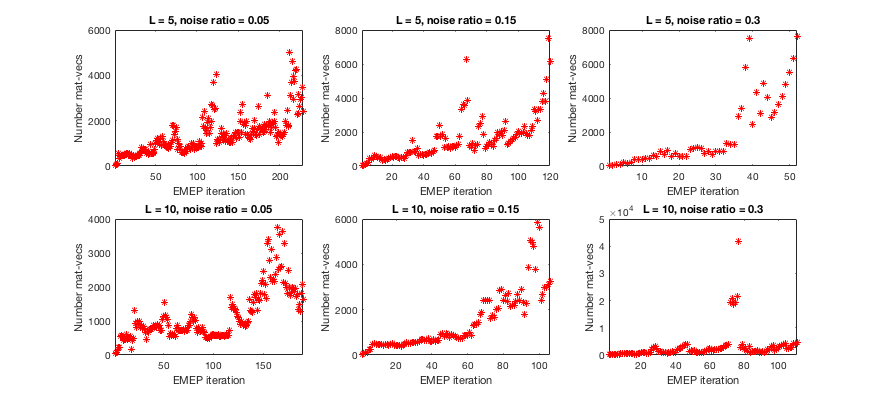
\includegraphics[scale=0.6]{EMEP_costs_num_mat_vecs} }\vspace{-0.4cm}
	\caption{Number of matrix-vector products for each iteration in the \emep \ for the six smaller models from Table \ref{Tab:EMEP_costs}	.}
\label{Fig:EMEP_costs_num_mat_vecs}
\end{figure}
% experiments.figure.noisyimage_costs

Figure \ref{Fig:EMEP_costs_num_mat_vecs} demonstrates that the number of matrix-vector products required for each \emep \ iterate varies greatly from earlier to later iterates.  
In each model, the later iterates account for the majority of the computational cost of the \emep.  
Additionally, some iterates require far more matrix-vector products than others (e.g., the iterates around $k=75$ in the bottom-right plot).
To help explain this change in computational costs, we now proceed to examine how the spectrum of the EMEP evolves.



\subsection{Evolving Spectrum Distribution} 	\label{Subsubsec:evol_mats-EMEP_spectrum_and_clustering}


We close this section by examining the evolving spectrum distribution of the \emep.
We find that the algebraically largest eigenvalues begin to cluster for  later EMEP iterates, likely causing those eigenvalue problems to be more difficult.
First, we examine the full spectrum of a few EMEP matrix iterates in Figure \ref{Fig:EMEP_full_spectrum}.




\begin{figure}[H]
\centering
\hbox{\hspace{-1.2cm} 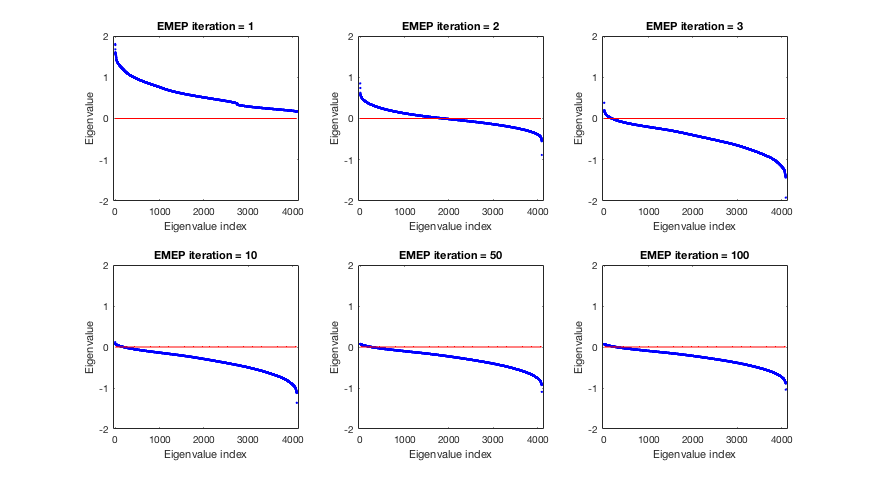
\includegraphics[scale=0.6]{EMEP_full_spectrum} }\vspace{-0.4cm}
	\caption{Spectrum of specific \emep \ matrix iterates $A_k$ for the model from Table \ref{Tab:EMEP_costs} with signal size $n = 4,096$, oversampling $L = 5$, and noise ratio $\epsilon_\text{rel} = 0.15$.}
\label{Fig:EMEP_full_spectrum}
\end{figure}
% experiments.figure.noisyimage_spectrumdist

As we see in Figure \ref{Fig:EMEP_full_spectrum}, the spectrum of the matrix iterates $A_k$ in the \emep \ shifts from completely positive for $A_1$ to mostly negative for later iterates.  This shift in spectrum is a consequence of optimizing the PLGD model (\ref{Eqn:PhaseLift-P-GD}).  The first matrix iterate $A_1 = \caA^*b$ will always be positive-semidefinite because the components of the observation $b=[b_1; b_2; \ldots; b_L]$ are all nonnegative and thus for all $x$ we have 
\[
x^*[\caA^*b]x 
	= \sum\limits_{\substack{j=1}}^{\substack{L}}
		[FC_jx]^* \textnormal{Diag}(b_j) F C_jx
	\geq 0.
\]
Since Algorithm \ref{Alg:PGD} minimizes the objective function $\lambda_1(\caA^*y_k)$, the algebraically largest eigenvalue $\lambda_1^{(k)}$ of $\caA^*y_k$ can be expected to decrease for later iterates $k$.  


As we will see in Section \ref{Subsec:evol_mats-IRAM}, the convergence rate of eigenvalue methods often depends on the distance between the desired eigenvalue $\lambda_j$ and the next algebraically largest eigenvalue $\lambda_{j+1}$.  Figure \ref{Fig:EMEP_largest_eigvals} depicts the 20 algebraically largest eigenvalues of the \emep \ iterates from Figure \ref{Fig:EMEP_full_spectrum}.


\begin{figure}[H]
\centering
\hbox{\hspace{-1.2cm} 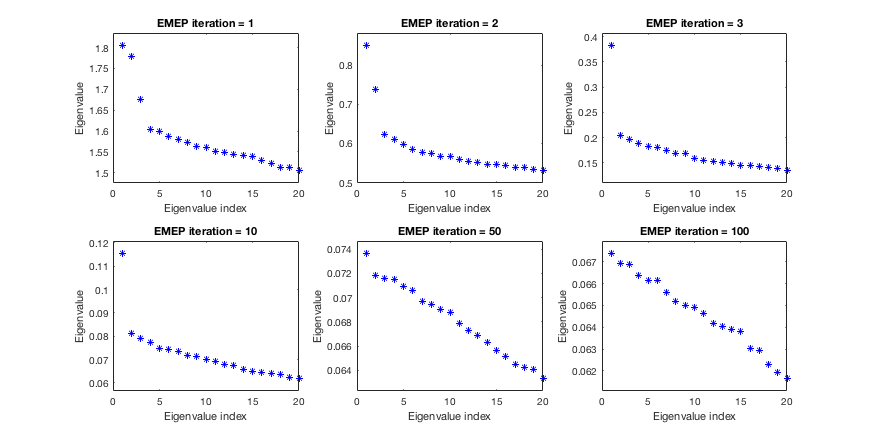
\includegraphics[scale=0.6]{EMEP_largest_eigvals} }\vspace{-0.4cm}
	\caption{Twenty algebraically largest eigenvalues of specific \emep \ matrix iterates $A_k$ for the model from Table \ref{Tab:EMEP_costs} with signal size $n = 4,096$, oversampling $L = 5$, and noise ratio $\epsilon_\text{rel} = 0.15$.}
\label{Fig:EMEP_largest_eigvals}
\end{figure}
% experiments.figure.noisyimage_spectrumdist

Figure \ref{Fig:EMEP_largest_eigvals} demonstrates that the algebraically largest eigenvalues of the matrix iterates $A_k$ cluster together as the \emep \ progresses.  
In general, this clustering in the \emep \ spectrum is expected.  
Section \ref{Subsec:PLGD_term_crit-stagnation} demonstrated that PLGD models with Gaussian noise (\ref{Eqn:PhaseLift-GD_Gaussian_noise}) typically have optimal primal matrices $X_\star$ with rank greater than one (see Table \ref{Tab:average_rank_soln_matrix_with_gaussian_dual_variable}).
And Corollary \ref{Cor:PLGD-optimality} (e) indicates that $\text{rank}(X_\star)$ is a lower bound on the multiplicity $r$ of the algebraically largest eigenvalue of the optimal dual matrix $\caA^*y_\star$.
Thus for later \emep \ iterates $k$, we can expect some $r$ algebraically largest eigenvalues $\lambda_1^{(k)}, \lambda_2^{(k)}, \ldots, \lambda_r^{(k)}$ to have a decreasing relative difference
\[
\frac{\lambda_i^{(k)} - \lambda_{i+1}^{(k)}}
	{\lambda_i^{(k)}}
\]
for $i = 1, 2, \ldots, r-1$.



The clustering of the algebraically largest eigenvalues as depicted in Figure \ref{Fig:EMEP_largest_eigvals} is known to slow the convergence rate of modern Krylov subspace methods.
Yet the choice of the parameters in these Krylov subspace methods can also affect their convergence rate significantly.
A thorough understanding of one such method (the implicitly restarted Arnoldi method) and its subroutines will help us to develop a new, adaptive strategy for choosing parameters for the \emep \ in Section \ref{Subsec:evol_mats-adaptive_IRAM}.






\section{The Implicitly Restarted Arnoldi Method}		\label{Subsec:evol_mats-IRAM}



% See following as references:
% http://www.cs.cornell.edu/~bindel/class/cs6210-f09/lec34.pdf
% http://people.inf.ethz.ch/arbenz/ewp/Lnotes/chapter11.pdf
%		Summarizes algorithms, math, convergence criteria, etc.
% ARPACK USERS GUIDE, p 53
%		Algo for IRAM on p 63

% Note: 
%	Prev	Golub
%	p		k, m
%	k		j
%	m		p (= m - j)
%	v		q


In this section we review the \textit{implicitly restarted Arnoldi method} (IRAM), a common large-scale eigenvalue method.  
First proposed by Sorensen \cite{sorensen1992implicit}, \cite{sorensen1997implicitly}, the IRAM is a combination of two essential algorithms.  
The \textit{$m$-step Arnoldi iteration} is used to build a matrix $Q_m$ of $m$ basis vectors which approximates the desired eigenspace.  
The \textit{$p$-step shifted QR iteration} restarts the matrix $Q_m$ with a specific strategy to damp unwanted eigenvalues, resulting in a smaller matrix $Q_j$ of $j<m$ basis vectors.  
Since the $m$-step Arnoldi iteration is an extension of the \textit{power method}, we first discuss the Power method before developing the IRAM.  
Altogether, the algorithms in this section are presented in the order depicted in Figure \ref{Fig:IRAM_flowchart}.

\begin{figure}[H] 
\centering
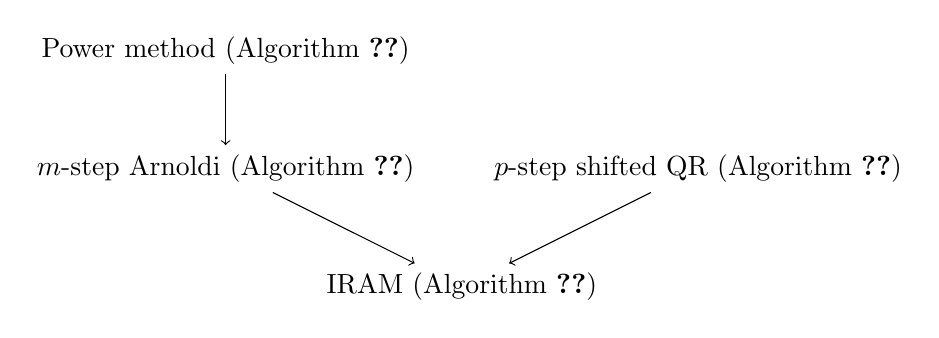
\begin{tikzpicture}
	\node (1) at (0,3) {Power method (Algorithm \ref{Alg:power_method})};
	\node (2) at (0,1.5) {$m$-step Arnoldi (Algorithm \ref{Alg:Arnoldi_iteration})};
	\node (3) at (6,1.5) {$p$-step shifted QR (Algorithm \ref{Alg:shifted_QR_iteration})};
	\node (4) at (3,0) {IRAM (Algorithm \ref{Alg:IRAM})};
	\draw[->] (1) -- (2);
	\draw[->] (2) -- (4);
	\draw[->] (3) -- (4);
\end{tikzpicture}
\caption{Dependency chart for the IRAM.}
\label{Fig:IRAM_flowchart}
\end{figure}

This section follows the treatment found in \cite[Chapters 8, 10]{golub2012matrix}, with occasional minor changes in notation.





\subsection{The Power Method} 			\label{Subsubsec:evol_mats-power_method}


The first method we consider is the \textit{power method}, a method for determining the largest magnitude eigenvalue $\lambda_1$ and corresponding eigenvector $v_1$ of a Hermitian matrix $A$.  The power method is based on the property that if $\lambda_1$ is strictly larger in magnitude than the next largest magnitude eigenvalue and the initial vector $q^{(0)}$ has a nonzero component in the direction of $v_1$ (i.e., $v_1^*q^{(0)} \neq 0$), then the sequence
\[
q^{(0)}, \frac{Aq^{(0)}}{||Aq^{(0)}||},  \frac{A^2q^{(0)}}{||A^2q^{(0)}||},  \frac{A^3q^{(0)}}{||A^3q^{(0)}||}, \ldots
\]
will have $v_1$ as its limit.  

Formally, Algorithm \ref{Alg:power_method} presents the power method as seen in \cite[Section 8.2.1]{golub2012matrix}.

\begin{algorithm}[H]
\caption{Power method}	\label{Alg:power_method}

\begin{algorithmic}[1]
	\Statex 	\textbf{Input:} Hermitian matrix $A$, initial approximate eigenvector $q^{(0)}$, relative tolerance $\textnormal{tol}_\textnormal{rel} > 0$.
	\Statex 	\textbf{Output:} Approximate largest magnitude eigenvalue $\lambda$ and the corresponding eigenvector $v$.
	\State		\textit{Initialize:} $q^{(0)} = q^{(0)}/||q^{(0)}||$, $\rho^{(0)} = [q^{(0)}]^*Aq^{(0)}$, $r^{(0)} = Au^{(0)} - \rho^{(0)}q^{(0)}$, $i= 1$.
	\While {\textit{not converged:} $ ||r^{(i)} || / (||Aq^{(i)}|| + |\rho^{(i)}|) > \textnormal{tol}_\textnormal{rel} $}
		\State		$z^{(i)} = Aq^{(i-1)}$
		\State		$q^{(i)} = z^{(i)} / ||z^{(i)}||$
		\State		$\rho^{(i)} = [q^{(i)}]^* z^{(i)}$
		\State		$r^{(i)} = Aq^{(i)} - \rho^{(i)}q^{(i)}$, $i = i + 1$
	\EndWhile
	\State		\textit{Return:} $(\lambda, v) = (\rho^{(i-1)} , q^{(i-1)})$.
\end{algorithmic}

\end{algorithm}


The simplicity of power method allows for insightful convergence results like the Theorem \ref{Thm:power_method_conv_rate}, in which we assume the matrix $A$ is real for clarity.

\begin{theorem}			\label{Thm:power_method_conv_rate}
Suppose $A \in \bbR^{n \times n}$ is symmetric with an eigenvalue decomposition
\[
V^*AV = \text{Diag}(\lambda_1, \lambda_2, \ldots, \lambda_n),
\]
where $V = [\ v_1 \ | \ v_2 \ | \cdots | \ v_n \ ]$ is orthogonal and $|\lambda_1| > |\lambda_2| \geq \cdots \geq |\lambda_n|$.  Let the vectors $q^{(i)}$ be generated by Algorithm \ref{Alg:power_method} and define $\theta_i \in [0, \pi/2]$ as 
\[
	\cos(\theta_i) = \left| v_1^Tq^{(i)} \right|.
\]
If $\cos(\theta_0) \neq 0$, then for $i = 0, 1, \ldots$ we have 
\begin{equation} 		\label{Eqn:power_method_conv_rate_1}
\left| \sin(\theta_i) \right| \leq \tan(\theta_0) \left| \frac{\lambda_2}{\lambda_1} \right|^i,
\end{equation}
\begin{equation} 		\label{Eqn:power_method_conv_rate_2}
\left| \lambda^{(i)} - \lambda_1 \right| \leq \max_{2 \leq j \leq n} \left| \lambda_1 - \lambda_i \right| \tan(\theta_0)^2 \left| \frac{\lambda_2}{\lambda_1} \right|^{2i}.
\end{equation}
\end{theorem}

\begin{proof}
See \cite[Theorem 8.2.1]{golub2012matrix}.
\end{proof}

Theorem \ref{Thm:power_method_conv_rate} establishes that the convergence rate of the power method (Algorithm \ref{Alg:power_method}) is dependent on the distance between $|\lambda_1|$ and $|\lambda_2|$.  If this distance $\epsilon = |\lambda_1| - |\lambda_2|$ is very small relative to $|\lambda_1|$, then we have
\[
\left| \frac{\lambda_2}{\lambda_1} \right| = \frac{|\lambda_1| - \epsilon}{|\lambda_1|} = 1 - \frac{\epsilon}{|\lambda_1|} \approx 1,
\]
and $|\sin(\theta_i)|$ in (\ref{Eqn:power_method_conv_rate_1}) may decreases very slowly.  







\subsection{The $m$-Step Arnoldi Iteration} 			\label{Subsubsec:evol_mats-Arnoldi}


The next method we consider is the \textit{$m$-step Arnoldi iteration} which extends the power method (Algorithm \ref{Alg:power_method}) to achieve a superior convergence rate.  An iteration of the power method generates a new approximate eigenvector ($q^{(i)}$ from steps 3 and 4) by normalizing the matrix-vector product of the previous vector.  In essence, the power method searches for the largest magnitude eigenvalue $\lambda_1$ and corresponding eigenvector $v_1$ of a matrix $A$ in the one-dimensional subspace $V = \textnormal{span} \{ Aq_1 \}$.  The $m$-step Arnoldi iteration extends the power method by searching for the Ritz pair (\ref{Def:Ritz_pair_val_vec}) ($\theta_1, u_1$) for $A$ with respect to the $m$-dimensional \textit{Krylov subspace}
\begin{equation}
\caK_m(A, q_1) = \textnormal{span}\{ q_1, Aq_1, A^2q_1, \ldots, A^{m-1}q_1 \}.
\label{Def:krylov_subspace}
\end{equation}
Algorithm \ref{Alg:Arnoldi_iteration} (as described in \cite[Algorithm 10.5.1]{golub2012matrix}) builds a unitary basis $Q_m$ of $\caK_m(A, q_1)$ which may be used to find the Ritz pair ($\theta_1, u_1$).
\begin{algorithm}[H]
\caption{$m$-step Arnoldi iteration}	\label{Alg:Arnoldi_iteration}

\begin{algorithmic}[1]
	\Statex		\textbf{Input:} Matrix $A \in \bbC^{n \times n}$, number of Arnoldi steps $m$, initial approximate eigenvector $q_1$.
	\Statex 	\textbf{Output:} Hessenberg matrix $H_m$, basis $Q_m$, residual $r_m$.
	\State		\textit{Initialize:} $q_1  = q_1 / ||q_1||$, \ \ $z = Aq_1$, \ \ $\alpha_1 = q_1^*z$, \ \ $r_1 = z - \alpha_1 q_1$, \ \ $Q_1 = [q_1]$, \ \ $H_1 = [\alpha_1]$.
	\For 			{$i = 1, \ldots, m-1$}
		\State	$\beta_i = ||r_i||$, \ \ $q_{i+1} = r_i / \beta_i$.
		\State	$Q_{i+1} = [Q_i \ | \ q_{i+1}]$, \ \ $\hat{H}_i = \begin{bmatrix}	H_i \\  \beta_i e_i^T	\end{bmatrix}$.
		\State	$z = Aq_{i+1}$.
		\State	$h = Q_{i+1}^*z$, \ \  $r_{i+1} = z - Q_{i+1}h$.
		\State	$H_{i+1} = [\hat{H}_i \ | \ h]$.
	\EndFor
	\State		\textit{Return:} $H_m, Q_m, r_m$.
\end{algorithmic}

\end{algorithm}

In order to obtain a Ritz pair ($\theta, u$) for $A$ with respect to $\caK_m(A, q_1)$, the $m$-step Arnoldi iteration generates an \textit{$m$-step Arnoldi decomposition}
\begin{equation} 		\label{Eqn:Arnoldi_decomp}
AQ_m = Q_m H_m + r_m e_m^*,
\end{equation}
where $H_m$ is an upper Hessenberg matrix.  If $(\theta, w)$ is an eigenpair for $H_m$ and $u = Q_mw$ then (\ref{Eqn:Arnoldi_decomp}) implies
\begin{equation} 			\label{Eqn:Arnoldi_decomp_Ritz_pairs}
(AQ_m - Q_mH_m)w = (A-\theta I) u = (e_m^*w)r_m.
\end{equation}
Additionally, steps 5 and 6 of Algorithm \ref{Alg:Arnoldi_iteration} indicate that $r_m$ is orthogonal to $\caK_m(A, q_1)$, and thus ($\theta, u$) is a Ritz pair for $A$ with respect to $\caK_m(A, q_1)$.  


The use of $\caK_m(A, q_1)$ in Algorithm \ref{Alg:Arnoldi_iteration} allows for superior convergence to Algorithm \ref{Alg:power_method}.  Note that the largest magnitude Ritz pair $(\theta_1, u_1)$ for $A$ with respect to $\caK_m(A, q_1)$ generated by Algorithm \ref{Alg:Arnoldi_iteration}  is guaranteed to be at least comparable to the $m$-th iterate of Algorithm \ref{Alg:power_method} since $A^{m-1}q_1 \in  \caK_m(A, q_1)$.  To compare the convergence rates of Algorithms \ref{Alg:power_method} and \ref{Alg:Arnoldi_iteration} more precisely, assume the matrix $A$ in real and symmetric.  Then the matrix $H_m$ returned by Algorithm \ref{Alg:Arnoldi_iteration} is tridiagonal and this algorithm is equivalent to the \textit{$m$-step Lanczos iteration} \cite[Algorithm 10.1.1]{golub2012matrix}.  In this case, we have the Theorem \ref{Thm:Lanczos_conv_rate}.  Note that this theorem involves \textit{Chebyshev polynomials} \cite[Section 4.4]{saad2011numerical}, a sequence of polynomials defined recursively as
\begin{equation} 			\label{Def:Chebyshev_polys}
c_k(x) = 2x c_{k-1}(x) - c_{k-2}(x)
\end{equation}
for $k \geq 2$, with $c_0 = 1$ and $c_2 = x$ .

\begin{theorem}   		\label{Thm:Lanczos_conv_rate}
Let $A \in \bbR^{n \times n}$ be symmetric with an eigenvalue decomposition
\[
V^*AV = \text{Diag}(\lambda_1, \lambda_2, \ldots, \lambda_n),
\]
where $V = [\ v_1 \ | \ v_2 \ | \cdots | \ v_n \ ]$ is orthogonal and $\lambda_1 \geq \lambda_2 \geq \cdots \geq \lambda_n$.  Suppose the $m$-step Arnoldi iteration (Algorithm \ref{Alg:Arnoldi_iteration}) is performed and $H_k$ is the tridiagonal matrix returned by this algorithm.  If $\theta_1$ is the algebraically largest eigenvalue of $H_m$, then
\begin{equation} 			\label{Eqn:Lanczos_thm_1}
\lambda_1 \geq \theta_1 \geq \lambda_1 - (\lambda_1 - \lambda_n) 
\left( \frac{\tan(\phi_1)}{c_{m-1}(1+2\rho_1)} \right)^2,
\end{equation}
where $\cos(\phi_1) = |q_1^Tv_1|$,
\begin{equation}		\label{Eqn:Lanczos_thm_2}
\rho_1 = \frac{\lambda_1 - \lambda_2}{\lambda_2 - \lambda_n},
\end{equation}
and $c_{m-1}(x)$ is the Chebyshev polynomial of degree $m-1$.
\end{theorem}

\begin{proof}
See \cite[Theorem 10.1.2]{golub2012matrix}.
\end{proof}

The convergence rate established in Theorem \ref{Thm:Lanczos_conv_rate} may also be applied to Algorithm \ref{Alg:power_method}, giving the Corollary \ref{Cor:Lanczos_cor_for_power_method}.

\begin{corollary} 			\label{Cor:Lanczos_cor_for_power_method}
Let $A \in \bbR^{n \times n}$ be symmetric and positive semidefinite with an eigenvalue decomposition
\[
V^*AV = \text{Diag}(\lambda_1, \lambda_2, \ldots, \lambda_n),
\]
where $V = [\ v_1 \ | \ v_2 \ | \cdots | \ v_n \ ]$ is orthogonal and $\lambda_1 \geq \lambda_2 \geq \cdots \geq \lambda_n \geq 0$.  Suppose $m$ steps of the power method (Algorithm \ref{Alg:power_method}) are performed and $\gamma_1 = \rho^{(m)}$ is the returned Ritz value.  Then
\begin{equation} 			\label{Eqn:Lanczos_cor_for_power_method}
\lambda_1 \geq \gamma_1 \geq \lambda_1 - (\lambda_1 - \lambda_n) 
\tan^2(\phi_1) \left( \frac{\lambda_2}{\lambda_1} \right)^{2(m-1)},
\end{equation}
where $\cos(\phi_1) = |q_1^Tv_1|$.
\end{corollary}

\begin{proof}
See \cite[Theorem 10.1.2]{golub2012matrix} and replace the Chebyshev polynomial in this proof with $p(x) = x^{k-1}$.
\end{proof}


The lower bounds in Theorem \ref{Thm:Lanczos_conv_rate} and Corollary \ref{Cor:Lanczos_cor_for_power_method} may be used to compare the expected convergence rates for Algorithms \ref{Alg:power_method} and \ref{Alg:Arnoldi_iteration}.  The following comparison is based on \cite[Section 10.1.6]{golub2012matrix}.  Assume $A \in \bbR^{n \times n}$ is symmetric and also positive semidefinite for clarity.  Assume Algorithms \ref{Alg:power_method} and \ref{Alg:Arnoldi_iteration} have been run for $m$ steps with the same initial vector $q_1$.  Let $\gamma_1 = \rho^{(m)}$ be the Ritz value for $A$ generated by step 5 of Algorithm \ref{Alg:power_method}.  And let $\theta_1$ be the Ritz value for $A$ with respect to $\caK_m(A, q_1)$ generated by the algebraically largest eigenvalue of $H_m$ from Algorithm \ref{Alg:Arnoldi_iteration}.  Then we may compare the lower bounds (\ref{Eqn:Lanczos_cor_for_power_method}) for $\gamma_1$ and (\ref{Eqn:Lanczos_thm_1}) for $\theta_1$ by comparing the values
\begin{equation} 		\label{Eqn:power_method_lower_bound}
P_{m-1} = \left( \frac{\lambda_2}{\lambda_1} \right)^{2(m-1)},
\end{equation}
\begin{equation}  	\label{Eqn:Lanczos_lower_bound}
L_{m-1} 
	= \frac{1}{\left[c_{m-1}\left(2\frac{\lambda_1}{\lambda_2} -1 \right)\right]^2} 
	\geq 	\frac{1}{\left[ c_{m-1}\left( 1 + 2 \rho_1 \right) \right]^2}.
\end{equation}
Table \ref{Tab:Lanczos_vs_power_method} compares $P_{m-1}$ and $L_{m-1}$ for a few values of $m$ and $\lambda_1/\lambda_2$.

\begin{table}[H]
\centering
\begin{tabular}{ |c|cc|cc| }
 \hline

 	&	\multicolumn{2}{c|}{$m = 10$}
 		&	\multicolumn{2}{c|}{$m = 20$}	\\
 $\lambda_1 / \lambda_2$	&	$P_{m-1}$	&	$L_{m-1}$
 		&	$P_{m-1}$	&	$L_{m-1}$		\\ 			
 \hline
$1.10$
	&	$1.8 \times 10^{-1}$ & $5.5 \times 10^{-5}$
		&	$2.7 \times 10^{-2}$ & $2.1 \times 10^{-10}$	\\
$1.01$
	&	$8.4 \times 10^{-1}$ & $1.0 \times 10^{-1}$
		&	$6.9 \times 10^{-1}$ & $2.0 \times 10^{-3}$	\\
 \hline
\end{tabular}
\caption{Lower bound terms (\ref{Eqn:power_method_lower_bound}) and (\ref{Eqn:Lanczos_lower_bound}) for Ritz values generated by Algorithms \ref{Alg:power_method} and \ref{Alg:Arnoldi_iteration} } \label{Tab:Lanczos_vs_power_method}
\end{table}

Table \ref{Tab:Lanczos_vs_power_method} demonstrates that the use of the Krylov subspace $\caK_m(A, 	q_1)$ in Algorithm \ref{Alg:Arnoldi_iteration} allows for superior convergence to Algorithm \ref{Alg:power_method}.  Yet this superior convergence rate is slowed somewhat when the desired eigenvalue $\lambda_1$ is close to $\lambda_2$.  For eigenvalue problems where the value $\lambda_1 / \lambda_2$ is very small (like later iterates of the \emep, as demonstrated in Figure \ref{Fig:EMEP_largest_eigvals}), we may seek to increase the number of steps $m$ in Algorithm \ref{Alg:Arnoldi_iteration}.  Yet increasing $m$ can be computationally prohibitive if the eigenvalue problem is very large, requiring significant memory to store $Q_m$ and significant computation to compute the eigenvalue decomposition of $H_m$.






\subsection{The $p$-Step Shifted QR Iteration} 			\label{Subsubsec:evol_mats-QR_iteration}


To take advantage of the convergence rate of Algorithm \ref{Alg:Arnoldi_iteration} for larger eigenvalue problems, the Arnoldi decomposition (\ref{Eqn:Arnoldi_decomp}) may be restarted with the \textit{$p$-step shifted QR iteration} developed by \cite{sorensen1992implicit} and discussed in \cite[Sections 10.5.2-3]{golub2012matrix}.  To develop this algorithm, assume we are seeking the $j$ algebraically largest eigenvalues of a Hermitian matrix $A \in \bbC^{n \times n}$ and we require that the $m$-step Arnoldi decomposition (\ref{Eqn:Arnoldi_decomp}) $AQ_m = Q_m H_m + r_m e_m^*$ has a fixed size $m > j$.  First we run Algorithm \ref{Alg:Arnoldi_iteration} with the initial vector $q_1$ to obtain $AQ_m = Q_m H_m + r_m e_m^*$.  Next, recall that the matrix $H_m$ may be used to identify the desired Ritz pairs $\{(\theta_i, u_i)\}_{i=1}^j$ for $A$ with respect to $\caK_m(A, q_1)$, as described in (\ref{Eqn:Arnoldi_decomp_Ritz_pairs}).  Yet $H_m$ also contains Ritz values $\theta_{j+1}, \ldots, \theta_m$ which correspond to unwanted eigenvalues of $A$.  To damp these unwanted Ritz values, we may select an appropriate degree $p = m-j$ filter polynomial $p(\lambda)$.  The $p$-step shifted QR iteration uses the filter polynomial
\begin{equation} 			\label{Eqn:filter_poly}
p(\lambda) = c \cdot (\lambda - \mu_1) (\lambda - \mu_2) \cdots (\lambda - \mu_p),
\end{equation}
where $c$ is a constant and the shift values $\mu_1 = \theta_{j+1}, \ldots, \mu_p = \theta_m$ are the $p$ unwanted Ritz values of $A$ with respect to $\caK_m(A, q_1)$.  Algorithm \ref{Alg:shifted_QR_iteration} (as described in \cite[Section 10.5.3]{golub2012matrix}) uses the filter polynomial (\ref{Eqn:filter_poly}) implicitly by applying $p$ shifted QR steps to $H_m$.
%(see \cite[Section 5.2]{golub2012matrix} for details regarding the QR factorization)
\begin{algorithm}[H]
\caption{$p$-step shifted QR iteration (implicit polynomial filtering)}	\label{Alg:shifted_QR_iteration}

\begin{algorithmic}[1]
	\Statex 	\textbf{Input:} Hessenberg matrix $H_m \in \bbC^{m \times m}$ and shift values $\mu_1, \ldots, \mu_p$.
	\Statex 	\textbf{Output:} Processed Hessenberg matrix $H_m^+ \in \bbC^{m \times m}$ and change of basis $V \in \bbC^{m \times m}$, with $H_m^+ = V^*H_mV$.
	\State		Set $H^{(0)} = H_m$.
	\For {$i = 1, \ldots, p$ }
		\State		\textit{QR factorization:} $H^{(i-1)} - \mu_i I = V_iR_i$.
		\State		\textit{Update:} $H^{(i)} = R_iV_i + \mu_iI$.
	\EndFor
	\State		Set $H_m^+ = H^{(p)}$, $V = V_1  V_2 \cdots V_p$.
	\State		\textit{Return:} $H_m^+, V$.
\end{algorithmic}

\end{algorithm}

Proposition \ref{Prop:Arnoldi_restart} establishes that Algorithm \ref{Alg:shifted_QR_iteration} implicitly applies the filter polynomial $p(\lambda)$ from (\ref{Eqn:filter_poly}) to the initial vector $q_1$ used to create the $m$-step Arnoldi decomposition (\ref{Eqn:Arnoldi_decomp}).

\begin{prop} 			\label{Prop:Arnoldi_restart}
Let $A \in \bbC^{n \times n}$ be Hermitian and $AQ_m = Q_mH_m + r_me_m^*$ be the $m$-step Arnoldi decomposition (\ref{Eqn:Arnoldi_decomp}) returned by Algorithm \ref{Alg:Arnoldi_iteration} with initial vector $q_1$.  And let $\mu_1, \ldots, \mu_p$ be the $p$ smallest algebraic eigenvalues of $H_m$.  Run Algorithm \ref{Alg:shifted_QR_iteration} with $H_m$ and $\mu_1, \ldots, \mu_p$ as inputs, and return $H_m^+$, $V = V_1 \cdots V_p$, and $R = R_p \cdots R_1$.

Then the restarted matrix $Q_+ = Q_mV$ will have the first column
\[
q_+ = Q_mV(:,1) = p(A)q_1,
\]
where $p(\lambda)$ is the filter polynomial (\ref{Eqn:filter_poly}) with constant $c = 1/R(1,1)$.
\end{prop}


\begin{proof}
See \cite[Section 10.5.3]{golub2012matrix}.
\end{proof}


\iffalse

\begin{proof}
First we must show that 
\begin{equation} 		\label{Eqn:filter_poly_proposition-VR}
VR = (H_m - \mu_1I) \cdots (H_m - \mu_pI).
\end{equation}

Using induction, we see that if $p=1$ then clearly (\ref{Eqn:filter_poly_proposition-VR}) holds.  If $p>1$, then let $\tilde{V}=V_1 \cdots V_{p-1}$ and $\tilde{R} = R_{p-1} \cdots R_1$, and note that $H^{(p-1)} = \tilde{V}^*H_m\tilde{V}$.  Then we have
\[
\begin{split}
VR & = \tilde{V}(V_pR_p)\tilde{R} 
	= \tilde{V} \left( H^{(p-1)} - \mu_pI \right) \tilde{R}
	= \tilde{V}\left( \tilde{V}^*H_m \tilde{V} - \mu_p I \right)\tilde{R}	\\
	& = \left(H_m - \mu_p I \right) \tilde{V}\tilde{R}
	= (H_m - \mu_p I) (H_m - \mu_1 I) \cdots (H_m - \mu_{p-1}I) 	\\
	&=  (H_m - \mu_1I) \cdots (H_m - \mu_pI),
\end{split}
\]
and (\ref{Eqn:filter_poly_proposition-VR}) holds.

Next, note that if the $m$-step Arnoldi decomposition (\ref{Eqn:Arnoldi_decomp}) is right-multiplied by $e_1$, then for all $\mu$ we have
\begin{equation} 			\label{Eqn:filter_poly_propostion-flip}
\left(A - \mu I \right)Q_me_1 = Q_m \left(H_m - \mu I \right) e_1.
\end{equation}

Then we have
\[
\begin{split}
q_+ 
	& = Q_mV(:,1) = Q_m \left[ \frac{1}{R(1,1)}VR e_1 \right] 	\\
	& 	= Q_m p(H_m) e_1 = p(A)Q_m e_1	\\
	& 	= p(A) q_1,
\end{split}
\]
where the third equality is given by (\ref{Eqn:filter_poly_proposition-VR}) and the fourth is given by (\ref{Eqn:filter_poly_propostion-flip}).
\end{proof}

\fi





After performing Algorithm \ref{Alg:shifted_QR_iteration}, we have the transformed $m$-step Arnoldi decomposition (\ref{Eqn:Arnoldi_decomp})
\begin{equation}			\label{Eqn:Arnoldi_decomp_transf_shifted_QR}
AQ_+ = Q_+H_+ + r_me_m^*V,
\end{equation}
where $V = V_1 \cdots V_p$ from Algorithm \ref{Alg:shifted_QR_iteration} and $Q_+ = Q_mV$.  As a consequence of the QR steps used in Algorithm \ref{Alg:shifted_QR_iteration}, we can also show that the first $j = m-p$ columns of (\ref{Eqn:Arnoldi_decomp_transf_shifted_QR}) form a new $j$-step Arnoldi decomposition.  Note that $V_1, \ldots, V_p$ are all upper Hessenberg due to the QR factorization in step 3 of Algorithm \ref{Alg:shifted_QR_iteration}.  Then $V$ has a lower band $p$ and $V(m, 1:m-p-1) = V(m, 1:j-1) = 0$, giving
\begin{equation} 			\label{Eqn:Arnoldi_decomp_transf_shifted_QR-part1}
r_me_m^*V(:, 1:j) = V(m,j)r_me_j^*.
\end{equation}
Also, $H_+$ is upper Hessenberg and thus $H_+(j+1:m, 1:j) = H_+(j+1,j)e_1e_j^*$, giving
\begin{equation} 		\label{Eqn:Arnoldi_decomp_transf_shifted_QR-part2}
\begin{split}
Q_+H_+(:, 1:j) 
	&	=  Q_+(:, 1:j) H_+(1:j, 1:j) + Q_+(:, j+1:m)H_+(j+1:m, 1:j) \\
	&	=	Q_+(:, 1:j) H_+(1:j, 1:j) +  H_+(j+1,j)Q_+(:,j+1)e_j^*.
\end{split}
\end{equation}

Therefore, if we set $Q_j = Q_+(:, 1:j) = Q_mV(:, 1:j)$, $H_j = H_+(1:j, 1:j)$, and $r_j = V(m,j)r_m + H_+(j+1,j)Q_+(:,j+1)$, then equations (\ref{Eqn:Arnoldi_decomp_transf_shifted_QR}-\ref{Eqn:Arnoldi_decomp_transf_shifted_QR-part2}) give the new $j$-step Arnoldi decomposition
\begin{equation}		\label{Eqn:Arnoldi_decomp_j-step_update}
\begin{split}
AQ_j  
	&	= AQ_+(:, 1:j) 	\\
	& = Q_+(:, 1:j)H_+(1:j, 1:j) + \left[V(m,j)r_m + H_+(j+1,j)Q_+(:,j+1) \right] e_j^*		\\
	& = Q_jH_j + r_je_j^*,
\end{split}
\end{equation}
and we may resume Algorithm \ref{Alg:Arnoldi_iteration} at step $j+1$.




\subsection{The Implicitly Restarted Arnoldi Method} 			\label{Subsubsec:evol_mats-IRAM}


Combining Algorithms \ref{Alg:Arnoldi_iteration} and \ref{Alg:shifted_QR_iteration} as described above, we have Algorithm \ref{Alg:IRAM} as presented in \cite[Section 10.5.3]{golub2012matrix}.

\begin{algorithm}[H]
\caption{Implicitly restarted Arnoldi method (IRAM)}	\label{Alg:IRAM}

\begin{algorithmic}[1]
	\Statex 	\textbf{Input:} Matrix $A \in \bbC^{n \times n}$, initial approximate eigenvector $q_1$, number of requested algebraically largest eigenvalues $j$, maximum Arnoldi decomposition (\ref{Eqn:Arnoldi_decomp}) size $m$.
	\Statex 	\textbf{Output:} Approximate algebraically largest eigenpairs $(\Lambda_j, V_j)$.
	\State		\textit{Initialize with Algorithm \ref{Alg:Arnoldi_iteration}:} Perform the $m$-step Arnoldi iteration with initial vector $q_1$ to obtain $AQ_m = Q_m H_m + r_m e_m^*$.
	\While {not converged}
		\State		Compute the eigenvalues $\theta_1, \ldots , \theta_m$ of $H_m$ and identify the $p = m-j$ (unwanted) shift values $\mu_1 = \theta_{j+1},  \ldots, \mu_p = \theta_m$.
		\State		\textit{Algorithm \ref{Alg:shifted_QR_iteration}:}  Perform the $p$-step shifted QR iteration to obtain the Hessenberg matrix $H_+$ and change of basis $V$.
		\State		\textit{Restart the Arnoldi factorization:} Set 
		$Q_j = Q_mV(:, 1:j)$,
		$H_j = H_+(1:j, 1:j)$,
		and $r_j = V(m,j)r_m + H_+(j+1,j)Q_+(:,j+1)$ per (\ref{Eqn:Arnoldi_decomp_j-step_update}).
		\State		\textit{Algorithm \ref{Alg:Arnoldi_iteration}:}  Beginning with $AQ_j = Q_jH_j + r_je_j^*$, perform steps $j+1, \ldots, m$ of the Arnoldi iteration to obtain $AQ_m = Q_m H_m + r_m e_m^*$.
	\EndWhile
	\State 		Compute the $j$ algebraically largest eigenvalues $\Lambda_j = \{ \lambda_1, \ldots, \lambda_j\}$ and corresponding eigenvectors $u_1, \ldots, u_j$ of $H_m$.  Set $V_j = [ \ Q_m u_1 \ | \cdots | \ Q_m v_j \ ]$.
	\State		\textit{Return:} $(\Lambda_j, V_j)$.
\end{algorithmic}

\end{algorithm}


The IRAM is the eigenvalue method we use in Section \ref{Subsec:evol_mats-adaptive_IRAM} to handle the \emep.  The choice of parameters $m$ (the Arnoldi decomposition size) and $j$ (number of requested eigenvalues) can greatly impact the efficiency of IRAM (see Section \ref{Subsec:evol_mats-adaptive_IRAM}).  For many large-scale eigenvalue problems, the IRAM is a very effective and convenient method.  Due to the implicit polynomial filtering in step 4 of IRAM, this method is particularly effective when the $j$ algebraically largest eigenvalues have modest separation from $\lambda_{j+1}$.  And since the IRAM only has two parameter choices, there is little optimization required by the user.

However, when $\lambda_j \approx \lambda_{j+1}$ and the Arnoldi decomposition size $m$ is not sufficiently large, the IRAM may require many iterations to achieve the desired tolerance. 
 As we will see in Section \ref{Subsec:evol_mats-adaptive_IRAM}, the appropriate choice of $m$ and $j$ in this circumstance may make the IRAM far more competitive.  
Yet choosing $m$ and $j$ without prior knowledge of the eigenvalue distribution is inherently heuristic.  
Additionally, if the inputted matrix $A$ is very large, then it may be prohibitive to store the $Q_m \in \bbC^{n \times m}$ in active memory.  In particular, if the image or signal $x$ being recovered in the PLGD problem has $n$ pixels, then $Q_m$ will require $m-$times as much storage space.  
Thus we proceed in the next section by considering an alternative Krylov subspace method which does not require parameter tuning, nor a large subspace to be held in memory.


Note that the IRAM is implemented in the numerical software package \texttt{ARPACK} (the ARnoldi PACKage) in FORTRAN 77 \cite{lehoucq1998arpack}.  Many numerical computing environments include large-scale eigenvalue methods which having bindings to ARPACK, including \texttt{eigs} in MATLAB, \texttt{eigs} and \texttt{eigsh} in the Python package SciPy, \texttt{eigs} in R, and \texttt{eigs} in the Julia package Arpack.jl. 







\section{A New Strategy for the EMEP}
\label{Subsec:evol_mats-adaptive_IRAM}


In this section we develop a new strategy which uses the IRAM (Algorithm \ref{Alg:IRAM}) to handle the \emep \ while adaptively changing one of the IRAM parameters based on the results from the previous EMEP iterates.
As discussed in Section \ref{Subsec:evol_mats-IRAM}, the IRAM has only two key parameters: the number of requested eigenvalues $r$ and the Arnoldi decomposition (\ref{Eqn:Arnoldi_decomp}) size $m$.
As we will see, the proper choice of these parameters can greatly reduce the number of matrix-vector products required for the EMEP.


We begin by examining the change in computational costs  (as measured by matrix-vector products) with respect to various \emep \ iterates $k$ and IRAM parameters $r$ in Figure \ref{Fig:Numerics-num_matvecs_orig_vs_optimal_params}.
In the original implementation of Algorithm \ref{Alg:PGD}, all EMEP iterates were handled using the IRAM with $r=2$ requested eigenvalues and Arnoldi decomposition size $m = \min \{  \max \{ 2r, 20 \}, n \}$, where $n$ is the size of the desired signal $x$.  
This choice of $m$ is equivalent to the default parameter setting in the IRAM solver \texttt{eigs} for MATLAB and evaluates to $m=20$ for $n \geq 20$.
Yet the plots in Figure \ref{Fig:Numerics-num_matvecs_orig_vs_optimal_params} demonstrate that choosing a fixed parameter $r=2$ can result in far more matrix-vector products than is optimal.


\begin{figure}[H]
\centering
\hbox{\hspace{-0.2cm} 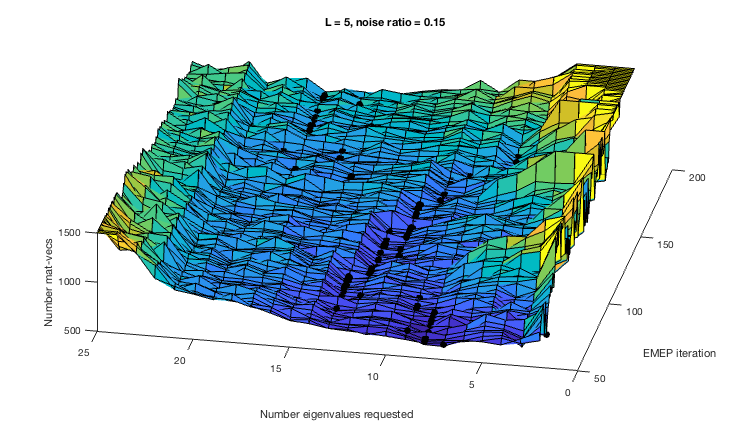
\includegraphics[scale=0.6]{Numerics-num_matvecs_orig_vs_optimal_params_1} }\vspace{1.0cm}
\hbox{\hspace{-0.8cm} 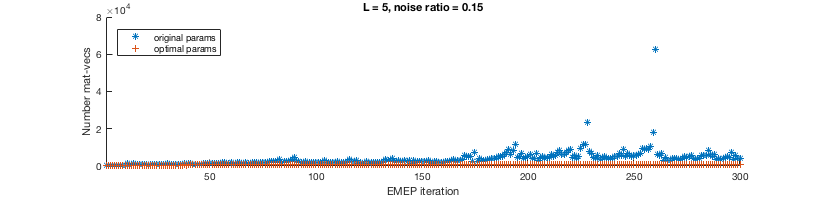
\includegraphics[scale=0.6]{Numerics-num_matvecs_orig_vs_optimal_params_2} }\vspace{0.0cm}
	\caption{
Performance results for an EMEP from a PLGD model with Gaussian noise	(\ref{Eqn:PhaseLift-GD_Gaussian_noise}) with noise ratio $\epsilon_\text{rel} = 0.15$, oversampling rate $L = 5$, and original signal from Figure \ref{Fig:parrot_signal_iterates} resized to $64 \times 64$ pixels.
Top: Number of matrix-vector products (capped at 1,500 for better viewing) for various EMEP iterates and number of requested eigenvalues $r$.  
Arnoldi decomposition size is set to $m = 40$ and black dots indicate the optimal parameter $r$ with the minimum number of products for each EMEP iterate.
Bottom: Plot of IRAM results for the EMEP with optimal parameters from top plot and fixed parameters $r=2$ and $m=20$.
	}
\label{Fig:Numerics-num_matvecs_orig_vs_optimal_params}
\end{figure}
% experiments.figure.noisyimage_adaptive_eig_full_exp




We now examine Figure \ref{Fig:Numerics-num_matvecs_orig_vs_optimal_params} to develop an adaptive strategy for choosing the number of requested eigenvalues $r$ for the sequence of EMEP iterates.
The top plot in Figure \ref{Fig:Numerics-num_matvecs_orig_vs_optimal_params} shows that the optimal choice of parameter $r$ typically changes only slightly between EMEP iterates.
However, the optimal parameter $r$ can increase quickly for later EMEP iterates (as we see around iterate 150 in the top plot in Figure \ref{Fig:Numerics-num_matvecs_orig_vs_optimal_params}).
Based on these observations, we may develop a strategy for choosing a sequence of parameters $r_1, r_2, \ldots, r_{maxit}$ as follows.
In order to measure change in the number of matrix-vector products for each iterate, we require that each pair of parameters $r_{k-1}$ and $r_k$ differ by at least one.
To select a new parameter $r_+$, we compare the two most recent choices for $r$ and the resulting number of matrix-vector products.
If these two choices for $r$ decreased the number of matrix-vector products, we continue to shift the value of $r$ in this direction by one unit; and otherwise we shift $r$ in the opposite direction.
We also allow $r$ to increase or decrease $r$ more rapidly by comparing the four most recent choices for $r$ and the resulting number of matrix-vector products using linear interpolation.
If these recent choices suggest the same shift as the first comparison, then we shift $r$ in this direction by two units rather than one.



This adaptive strategy for choosing the number of requested eigenvalues $r_k$ for each \emep \ iterate $k$ has the following steps.
First, we select a fixed Arnoldi decomposition size $m$ and initialize $r_1=r_{min}$ and $r_2 = r_1+1$ (where $r_{min}=2$, and $r_{max} = \min\{ 30, m-5 \}$, and we set the default value $m=40$).  
At each step $k \geq 2$ we update $r_{k+1} =  r_k + \delta$, where $\delta \in \{-2, -1, 1, 2\}$ is a shift based on the number of requested eigenvalues $r_k, r_{k-1}, \ldots$ and number of matrix-vector products $t_k, t_{k-1}, \ldots$ for the previous eigenvalues problems.
The shift $\delta$ is computed as follows.
First, we determine a \textit{$2$-step shift value} $\delta_2 \in \{-1, 1\}$ based on $r_{k-1}, r_k$ and $t_{k-1}, t_k$.
If $r_k > r_{k-1}$ and $t_k < t_{k-1}$ then the number of matrix-vector products in the \emep \ decreased as the number of requested eigenvalues was increased, suggesting we should shift $r_k$ by $\delta_2 = 1$.
By the same reasoning for the other three inequality cases, we define the
\textit{$2$-step shift value} as
\begin{equation}				\label{Eqn:adaptive_delta_2}
\delta_2 = \sign(r_k - r_{k-1}) \cdot \sign(t_{k-1} - t_k),
\end{equation}
where $\sign(0)$ is defined as $1$.
Next, if $k \geq 4$ then we compute a linear interpolation of the past four requested eigenvalue numbers and matrix-vector products by solving
\begin{equation} 			\label{Eqn:adaptive_delta_4_lin_interp_prob}
\min_{\alpha, \beta} || y - \alpha e - \beta x ||,
\end{equation}
where $y = [t_{k-3}; t_{k-2}; t_{k-1}; t_k]$ is the vector of matrix-vector product values, $x = [r_{k-3}; r_{k-2}; r_{k-1}; r_k]$ is the vector of the number of requested eigenvalues, and $e = [1;1;1;1]$.
If the solution to (\ref{Eqn:adaptive_delta_4_lin_interp_prob}) has $\beta > 0$ then the past four eigenvalue problems suggest that $t_i$ increases with $r_i$, and thus we should decrease $r_k$.
Thus we have the \textit{$4$-step shift value}
\begin{equation}			\label{Eqn:adaptive_delta_4}
\delta_4 = -\sign(\beta),
\end{equation}
where $\beta$ is determined by (\ref{Eqn:adaptive_delta_4_lin_interp_prob}).
If $\delta_2 = \delta_4$, then the $2$-step (\ref{Eqn:adaptive_delta_2}) and $4$-step equations (\ref{Eqn:adaptive_delta_4}) both suggest we should shift in the direction of $\delta_2$, and we select the shift $\delta = 2\delta_2$.
If $\delta_2 \neq \delta_4$ then we rely on the $2$-step equation (\ref{Eqn:adaptive_delta_2}) and select the shift value $\delta = \delta_2$.
Finally, if $r_k = r_{min}$ then we set $\delta = 1$ and if $r_k = r_{max}$ the we set $\delta = -1$.
Altogether, these steps lead to \textit{the IRAM with adaptive parameter selection} for the \emep.



\begin{algorithm}[H]
\caption{The IRAM with adaptive parameter selection for the \emep}	\label{Alg:adaptive_IRAM}

\begin{algorithmic}[1]
	\Statex 	\textbf{Input:} Sequence of matrices $\{ A_k \}_{k=1}^{maxit}$ from the \emep, Arnoldi decomposition (\ref{Eqn:Arnoldi_decomp})  size $m$ (default parameter $m = 40$).
	\Statex 	\textbf{Output:} \emep \ solution eigenpairs $\{ (\lambda_1^{(k)}, v_1^{(k)}) \}_{k=1}^{maxit}$ and  $\{ (\lambda_2^{(k)}, v_2^{(k)}) \}_{k=1}^{maxit}$.
	\State		\textit{Initialize:} $r_{min}=2$, $r_{max} = \min\{ 30, m-5 \}$, $r_1=r_{min}$, $t_0=-1$, $k=1$.
	\While {$k \leq maxit$}
		\State		\textit{Algorithm \ref{Alg:IRAM}:} Perform IRAM with matrix $A_k$, number of requested algebraically largest eigenvalues $r_k$, and maximum Arnoldi decomposition size $m$.  Return eigenpairs $(\lambda_1^{(k)}, v_1^{(k)} )$, $(\lambda_2^{(k)}, v_2^{(k)} )$ and number of matrix-vector products $t_k$.
		\If		{$r_k = r_{min}$}
			\State 		$r_{k+1} = r_k + 1$
		\ElsIf 	{$r_k = r_{max}$}
			\State		$r_{k+1} = r_k - 1$
		\ElsIf	{$k < 4$}
			\State		Compute $2$-step shift value $\delta_2$ from (\ref{Eqn:adaptive_delta_2}) and set $\delta = \delta_2$
			\State		$r_{k+1} = r_k + \delta$
		\Else
			\State 		Compute $2$-step shift value $\delta_2$ from (\ref{Eqn:adaptive_delta_2}) and $4$-step shift value $\delta_4$ from (\ref{Eqn:adaptive_delta_4})
			\If						{$\delta_2 = \delta_4$}
				\State		Set $\delta = 2\delta_2$
			\Else
				\State 			Set $\delta = \delta_2$
			\EndIf
			\State		$r_{k+1} =\min \{ \max \{ r_k + \delta, r_{min} \}, r_{max} \}$
		\EndIf
		\State		$k = k+1$
	\EndWhile
	\State		\textit{Return:} $\{ (\lambda_1^{(k)}, v_1^{(k)}) \}_{k=1}^{maxit}$ and  $\{ (\lambda_2^{(k)}, v_2^{(k)}) \}_{k=1}^{maxit}$.
\end{algorithmic}

\end{algorithm}



Note that the only parameter in Algorithm \ref{Alg:adaptive_IRAM} is the Arnoldi decomposition (\ref{Eqn:Arnoldi_decomp}) size $m$, which determines the size of the basis $Q_m \in \bbC^{n \times m}$ in the Arnoldi decomposition $AQ_m = Q_mH_m + r_me_m^*$.  
The choice of $m$ is a trade-off between computational efficiency and data storage constraints.
We seek the smallest value $m$ possible, since $Q_m$ must be stored in random-access memory and each column of $Q_m$ is the size of the desired signal $\bar{x}$ in the phase retrieval problem (\ref{Eqn:phase_retrieval}).
However, as we will see in Section \ref{Subsec:evol_mats-correl_btwn_EMEP_and_IRAM}, $m$ must be sufficiently large for the shifted QR iteration (Algorithm \ref{Alg:shifted_QR_iteration}) in the IRAM to handle the \emep \ efficiently.  
For now we will let $m=40$ to demonstrate the behavior of Algorithm \ref{Alg:adaptive_IRAM}.



We close this section by showing that Algorithm \ref{Alg:adaptive_IRAM} selects a sequence $r_1, r_2, \ldots r_{maxit}$ which varies significantly and generally tracks the optimal choice of the parameter $r$ for each \emep \ iterate.

\begin{figure}[H]
\centering
\hbox{\hspace{-1.0cm} 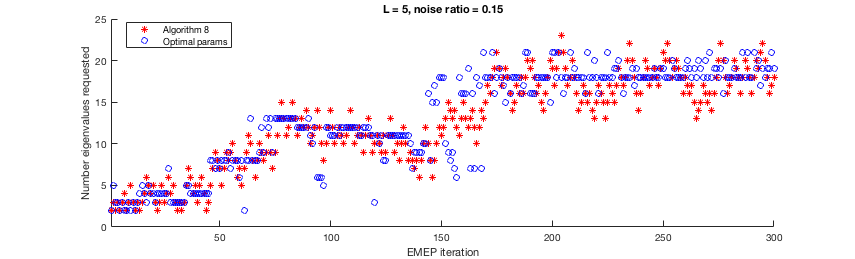
\includegraphics[scale=0.6]{Numerics-num_eigs_ada_vs_opt_1} }\vspace{0.6cm}
\vspace{0.2cm}
	\caption{
	Plot comparing Algorithm \ref{Alg:adaptive_IRAM} with the optimal choice of parameter $r$ (number of requested eigenvalues in the IRAM).
	 The \emep \ is from Figure \ref{Fig:Numerics-num_matvecs_orig_vs_optimal_params} and Arnoldi decomposition (\ref{Eqn:Arnoldi_decomp}) size is $m=40$.
	}
\label{Fig:Numerics-num_eigs_ada_vs_opt_one_plot}
\end{figure}
% experiments.figure.noisyimage_adaptive_eig_full_exp

Figure \ref{Fig:Numerics-num_eigs_ada_vs_opt_one_plot} shows that the parameter values $r_k$ chosen by Algorithm \ref{Alg:adaptive_IRAM} effectively track the optimal parameters for the IRAM.  
For the majority of iterates, the value $r_k$ is within two units from the optimal parameter value.
As we will see in Section \ref{Subsec:evol_mats-correl_btwn_EMEP_and_IRAM}, these changes in $r_k$ are related to the evolving spectrum of the \emep.




 


\section{Spectrum Distribution and IRAM Behavior}
\label{Subsec:evol_mats-correl_btwn_EMEP_and_IRAM}



In this section we examine an observed correlation between the clustering of the algebraically largest eigenvalues in the \emep \ and the convergence behavior of the IRAM (Algorithm \ref{Alg:IRAM}) for various parameters.
As we saw in Section \ref{Subsec:PLGD_term_crit-stagnation}, PLGD models with Gaussian noise (\ref{Eqn:PhaseLift-GD_Gaussian_noise}) typically have optimal EMEP matrices $\caA^*y_\star$ for which the algebraically largest eigenvalue has multiplicity greater than one.
Thus we may expect the algebraically largest eigenvalues in the EMEP to cluster for later iterates.

In Section \ref{Subsubsec:evol_mats-correl_clustering_IRAM_param} we examine two PLGD models and show that as the eigenvalues in the EMEP begin to cluster, the \textit{optimal} IRAM parameter $\bar{r}$ (i.e., the number of requested eigenvalues $r$ with the minimum number of matrix-vector products) increases such that $\lambda_{\bar{r}+1}$ is not clustered with $\lambda_1, \lambda_2, \ldots, \lambda_{\bar{r}}$.
We also see that the value $r_k$ chosen by Algorithm \ref{Alg:adaptive_IRAM} properly tracks the optimal parameter $\bar{r}_k$ for these two PLGD models.
Next, Section \ref{Subsubsec:evol_mats-default_Arnoldi_decomp_size} uses these two PLGD models to demonstrate that the Arnoldi decomposition (\ref{Eqn:Arnoldi_decomp}) size $m=40$ is sufficiently large for the IRAM to perform efficiently, and thus $m=40$ is an appropriate default parameter for Algorithm \ref{Alg:adaptive_IRAM}.





To illustrate these observations, we focus on the EMEP of two particular PLGD models with Gaussian noise (\ref{Eqn:PhaseLift-GD_Gaussian_noise}) for which the sequence of parameters $r_1, r_2, \ldots r_{maxit}$ chosen by Algorithm \ref{Alg:adaptive_IRAM} varies greatly.

\begin{figure}[H]
\centering
\hbox{\hspace{-1.1cm} 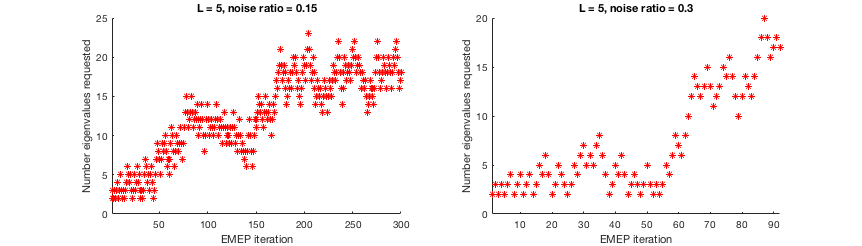
\includegraphics[scale=0.6]{Numerics-num_eigs_req_ada_2_exps} }\vspace{0.0cm}
	\caption{
Number of requested eigenvalues $r$ chosen by Algorithm \ref{Alg:adaptive_IRAM} for the \emep \ from two PLGD models with Gaussian noise (\ref{Eqn:PhaseLift-GD_Gaussian_noise}), with noise ratio $\epsilon_\text{rel}=0.15, 0.30$, oversampling rate $L=5$, and original signal from Figure \ref{Fig:parrot_signal_iterates} resized to $64 \times 64$ pixels.
}
\label{Fig:Numerics-num_req_eigs_2_exps}
\end{figure}
% experiments.figure.noisyimage_adaptive_eig_full_exp



For both PLGD models in Figure \ref{Fig:Numerics-num_req_eigs_2_exps}, changes in the EMEP caused Algorithm \ref{Alg:adaptive_IRAM} to increase the number of requested eigenvalues $r_k$ significantly from early to later iterates $k$.
Yet the value of $r_k$ increased at a quicker rate for the experiment in Figure \ref{Fig:Numerics-num_req_eigs_2_exps} with $L=5$ and $\epsilon_\text{rel} = 0.30$.
As we will see in Section \ref{Subsubsec:evol_mats-correl_clustering_IRAM_param}, this quick increase from $r_{55}=3$ to $r_{70}=13$ coincides with a sudden clustering of the algebraically largest eigenvalues in the EMEP.





\subsection{Eigenvalue Clustering and IRAM Parameter Choice}		\label{Subsubsec:evol_mats-correl_clustering_IRAM_param}




We now show that the PLGD models in Figure \ref{Fig:Numerics-num_req_eigs_2_exps} exhibit a correlation between the spectrum distribution of the \emep \ and the convergence behavior of the IRAM (Algorithm \ref{Alg:IRAM}).
For these two models, as the algebraically largest eigenvalues $\lambda_1, \lambda_2, \ldots, \lambda_{m-1}, \lambda_{m}$ of the EMEP begin to cluster, 
the IRAM converges much faster if the number of requested eigenvalues $r<m$ is large enough such that $\lambda_{r+1}$ is not clustered with $\lambda_1, \lambda_2, \ldots, \lambda_r$.
Thus, as Algorithm \ref{Alg:adaptive_IRAM} explicitly tracks the optimal sequence of parameters $\bar{r}_k$, this algorithm implicitly tracks the clustering of the algebraically largest eigenvalues in the EMEP.
To demonstrate these observations, we consider various EMEP iterates $k$ and number of requested eigenvalues $r$, and plot the numbers of matrix-vector products for the IRAM as well as the eigenvalue difference $\lambda_{r+1} - \lambda_r$.
Figures \ref{Fig:Numerics-surf_mvs_eig_diffs_1} and \ref{Fig:Numerics-surf_mvs_eig_diffs_2} depict about half of the EMEP iterates from the two PLGD models in Figure \ref{Fig:Numerics-num_req_eigs_2_exps}, so we may focus on the regions where $r_k$ in Algorithm \ref{Alg:adaptive_IRAM} varies greatest.





\begin{figure}[H]
\centering
\hbox{\hspace{-0.2cm} 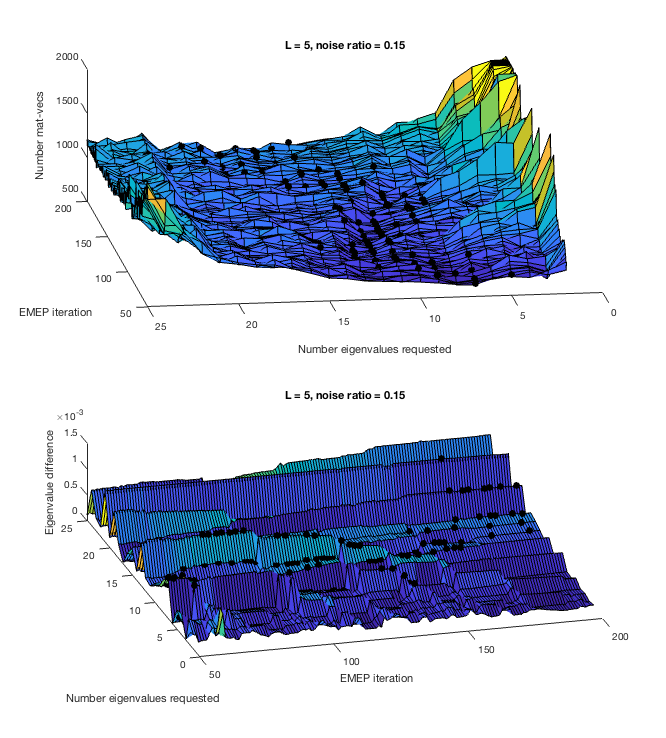
\includegraphics[scale=0.65]{Numerics-surf_num_mvs_and_eig_diffs_1} }\vspace{0.0cm}
	\caption{Behavior of Algorithm \ref{Alg:adaptive_IRAM} for the experiment from Figure \ref{Fig:Numerics-num_req_eigs_2_exps} with $L=5$, $\epsilon_\text{rel}=0.15$.  Top: Number of matrix-vector products (capped at 2,000 for better viewing) for each \emep \ iterate $k$ and number of requested eigenvalues $r$. Bottom: eigenvalue differences $\lambda_r - \lambda_{r+1}$ for each \emep \ iterate $k$ and number of requested eigenvalues $r$.  Black dots in both plots indicate the value $r_k$ chosen by Algorithm \ref{Alg:adaptive_IRAM}.}
\label{Fig:Numerics-surf_mvs_eig_diffs_1}
\end{figure}
% experiments.figure.noisyimage_adaptive_eig_full_exp



\begin{figure}[H]
\centering
\hbox{\hspace{-0.2cm} 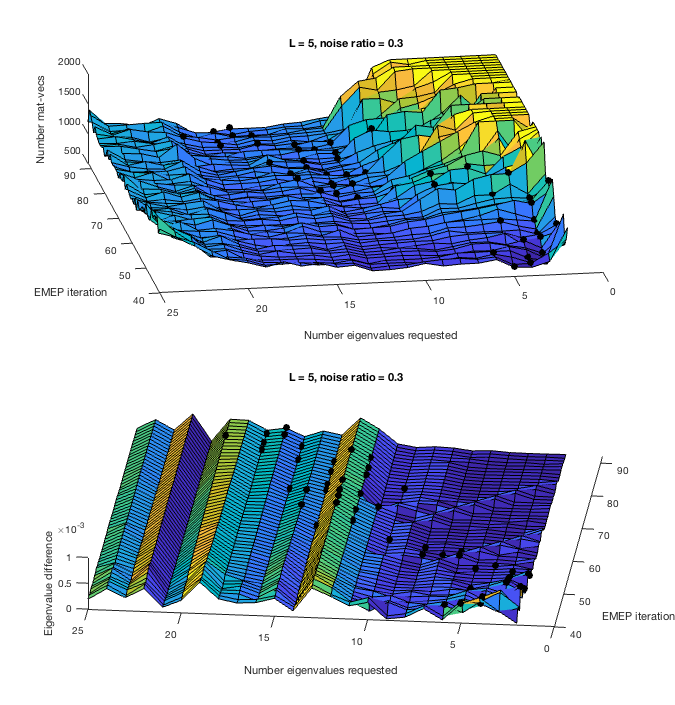
\includegraphics[scale=0.65]{Numerics-surf_num_mvs_and_eig_diffs_2} }\vspace{0.0cm}
	\caption{Behavior of Algorithm \ref{Alg:adaptive_IRAM} for the experiment from Figure \ref{Fig:Numerics-num_req_eigs_2_exps} with $L=5$, $\epsilon_\text{rel}=0.30$.  Top: Number of matrix-vector products (capped at 2,000 for better viewing) for each \emep \ iterate $k$ and number of requested eigenvalues $r$. Bottom: eigenvalue differences $\lambda_r - \lambda_{r+1}$ for each \emep \ iterate $k$ and number of requested eigenvalues $r$.  Black dots in both plots indicate the value $r_k$ chosen by Algorithm \ref{Alg:adaptive_IRAM}.}
\label{Fig:Numerics-surf_mvs_eig_diffs_2}
\end{figure}
% experiments.figure.noisyimage_adaptive_eig_full_exp





In Figures \ref{Fig:Numerics-surf_mvs_eig_diffs_1} and \ref{Fig:Numerics-surf_mvs_eig_diffs_2} we see that the clustering of the algebraically largest eigenvalues corresponds to an increase in the optimal number of requested eigenvalues $\bar{r}_k$ for later \emep \ iterates $k$.
In Figure \ref{Fig:Numerics-surf_mvs_eig_diffs_1}, the eigenvalues $\lambda_1, \lambda_2, \ldots, \lambda_{10}$ cluster around iterates $125 \leq k \leq 175$; and likewise the optimal parameter $\bar{r}_{125} \approx 10$ increases to $\bar{r}_{175} \approx 18$.
Figure \ref{Fig:Numerics-surf_mvs_eig_diffs_2} depicts a similar shift, where the eigenvalues $\lambda_1, \lambda_2, \ldots, \lambda_{10}$ cluster around iterates $50 \leq k \leq 70$, and the optimal parameter increases to $\bar{r}_{70} \approx 15$.
In the case of Figure \ref{Fig:Numerics-surf_mvs_eig_diffs_2}, the most tightly clustered eigenvalues $\lambda_1, \lambda_2, \ldots, \lambda_{8}$ also correspond to parameter values $r = 2, 3, \ldots, 7$ for which the IRAM required the greatest number of matrix-vector products to converge.



This observed correlation between eigenvalue clustering and a change in the convergence rate of the IRAM may be related to the subroutines used in the IRAM.
As discussed in Section \ref{Subsec:evol_mats-IRAM}, the IRAM is based on the following two algorithms.
Given a Hermitian matrix $A \in \bbC^{n \times n}$, the $m$-step Arnoldi iteration (Algorithm \ref{Alg:Arnoldi_iteration}) generates a set of Ritz pairs $(\theta_1, u_1), (\theta_2, u_2), \ldots, (\theta_m, u_m)$ for $A$ with respect to $\caK_m(A, q_1)$.
Next, the $p$-step shifted QR iteration (Algorithm \ref{Alg:shifted_QR_iteration}) restarts the Arnoldi decomposition (\ref{Eqn:Arnoldi_decomp}) by attempting to damp the unwanted part of the spectrum using the Ritz values $\{ \theta_{r+1}, \theta_{r+2}, \ldots, \theta_m \}$ (where $m = r + p$).
Assume we have an EMEP matrix iterate $A_k$ with some number $s$ of clustered algebraically largest eigenvalues, $\lambda_1 \approx \lambda_2 \approx \cdots \approx \lambda_s$; 
and assume we select the number of requested eigenvalues $r < s$.
When the IRAM builds an Arnoldi decomposition (\ref{Eqn:Arnoldi_decomp}), the $s$ largest Ritz values of $A_k$ with respect to $\caK_m(A_k, q_1)$ may include values $\theta_{r+1}, \theta_{r+2}, \ldots, \theta_s$ which are close approximations to the desired eigenvalues.
Thus when the shift values $\mu_1 = \theta_{r+1}, \mu_2 = \theta_{r+2}, \ldots, \mu_{s-r} = \theta_{s}, \ldots, \mu_p = \theta_m$ are passed to the $p$-step shifted QR iteration, the implicit polynomial filter (\ref{Eqn:filter_poly}) will include values $\mu_1, \mu_2, \ldots, \mu_{s-r}$ which damp the desired part of the spectrum.
Thus, if $r < s$ we may expect the IRAM to converge more slowly.
However, if we select the number of requested eigenvalues $r > s$, then the shift values used in the $p$-step shifted QR iteration will always include parts of the spectrum which we want to damp and we may expect the IRAM to converge more quickly. 


Figures \ref{Fig:Numerics-surf_mvs_eig_diffs_1} and \ref{Fig:Numerics-surf_mvs_eig_diffs_2} also demonstrate that Algorithm \ref{Alg:adaptive_IRAM} properly tracks the optimal number of requested eigenvalues $\bar{r}_k$ as this value changes.
In particular, Figure \ref{Fig:Numerics-surf_mvs_eig_diffs_2} indicates that $\bar{r}_k$ increased quickly from iterates $k = 50$ to $k = 70$.
Likewise, Algorithm \ref{Alg:adaptive_IRAM} increased $r_k$ by two units for several iterates $55 \leq k \leq 70$ (see Figure \ref{Fig:Numerics-num_req_eigs_2_exps}).
These two-unit increases were the result of Algorithm \ref{Alg:adaptive_IRAM} properly identifying a quick increase in the number of matrix-vector products $t_k$ for smaller values $r_k$.
Recall that Algorithm \ref{Alg:adaptive_IRAM} determines the update $r_{k+1}$ using two-point and four-point linear interpolations (equations (\ref{Eqn:adaptive_delta_2}) and (\ref{Eqn:adaptive_delta_4_lin_interp_prob}), respectively) of the previous parameters $r_k$ and $t_k$.
For the PLGD model in Figure \ref{Fig:Numerics-surf_mvs_eig_diffs_2}, both of these interpolations agreed (i.e., $\delta_2=1$ in (\ref{Eqn:adaptive_delta_2}) was equal to $\delta_4=1$ in (\ref{Eqn:adaptive_delta_4})) for several iterates $55 \leq k \leq 70$.
Thus Algorithm \ref{Alg:adaptive_IRAM} quickly increased $r_k$, avoiding excessive matrix-vector multiplications.







\subsection{Selecting the Arnoldi Decomposition Size}		\label{Subsubsec:evol_mats-default_Arnoldi_decomp_size}



Next we show that the default parameter setting $m = 40$ in Algorithm \ref{Alg:adaptive_IRAM} is sufficiently large to minimize the number of matrix-vector products in the EMEP in the models from Figure \ref{Fig:Numerics-num_req_eigs_2_exps}.
To demonstrate that $m=40$ is appropriate, we will examine a more difficult eigenvalue problem (i.e., later iterate) from each of these models.
Figure \ref{Fig:Numerics-surf_mvs_for_m_vs_j} depicts the number of matrix-vector products for various IRAM parameters $r$ and $m$ for an iterate from each model.


\begin{figure}[H]
\centering
\hbox{\hspace{0.3cm} 
	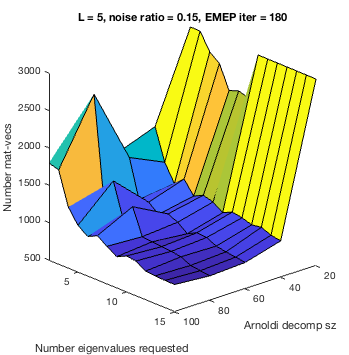
\includegraphics[scale=0.6]{Numerics-surf_mvs_for_m_vs_j_1}
	\hspace{0.5cm}
	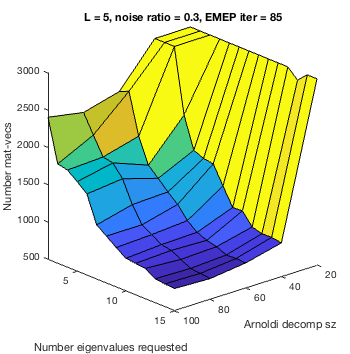
\includegraphics[scale=0.6]{Numerics-surf_mvs_for_m_vs_j_2} 
			}
	\vspace{0.0cm}
	\caption{
Number of matrix-vector products (capped at 3,000 for better viewing) for individual \emep \ iterates with varying number of requested eigenvalues $r$ and Arnoldi decomposition (\ref{Eqn:Arnoldi_decomp}) size $m$.  
Left: EMEP iterate 180 from Figure \ref{Fig:Numerics-surf_mvs_eig_diffs_1}.
Right: EMEP iterate 85 from Figure \ref{Fig:Numerics-surf_mvs_eig_diffs_2}.
	}
\label{Fig:Numerics-surf_mvs_for_m_vs_j}
\end{figure}
% experiments.figure.noisyimage_adaptive_eig_full_exp




Figure \ref{Fig:Numerics-surf_mvs_for_m_vs_j} suggests that we should not select IRAM parameters below $r = 9$ and $m = 40$ for the EMEP iterate in the left plot, nor should we select parameters below $r = 12$ and $m = 40$ for the EMEP iterate in the right plot.  
Yet there is no significant benefit to selecting larger parameter values.
Since the EMEP iterates in Figure \ref{Fig:Numerics-surf_mvs_for_m_vs_j} represent later, more difficult eigenvalue problems, this figure suggests that $m = 40$ is sufficiently large for all iterates.
Thus we select a fixed Arnoldi decomposition (\ref{Eqn:Arnoldi_decomp}) size $m = 40$ for Algorithm \ref{Alg:adaptive_IRAM}.






 
\newpage


\chapter{Experimental Results}
\label{Sec:Numerics}


This chapter examines the performance of Algorithm \ref{Alg:PGD} when we apply the modifications established in Chapters \ref{Sec:PLGD_term_crit} and \ref{Sec:evol_mats}.
Using the new termination conditions (\ref{Eqn:term_crit_new-primal_difference}) and (\ref{Eqn:term_crit_new-dual_difference}) for Algorithm \ref{Alg:PGD}, we examine the efficiency of the IRAM with adaptive parameter selection (Algorithm \ref{Alg:adaptive_IRAM}) for a variety of noisy phase retrieval problems.
First, we demonstrate that Algorithm \ref{Alg:adaptive_IRAM} is more efficient than the original IRAM (Algorithm \ref{Alg:IRAM}) parameter settings for a variety of PLGD models with Gaussian noise (\ref{Eqn:PhaseLift-GD_Gaussian_noise}).
We observe that Algorithm \ref{Alg:adaptive_IRAM} typically reduces the number of matrix-vector products in the EMEP by at least $50\%$ as compared with the original IRAM settings.
Next, we show that Algorithm \ref{Alg:adaptive_IRAM} is nearly optimal as a method for choosing the ideal number of requested eigenvalues $r_k$ corresponding to the minimum number of matrix-vector products necessary for each EMEP iteration.
Finally, we demonstrate that the Arnoldi decomposition (\ref{Eqn:Arnoldi_decomp}) size parameter $m = 40$ for Algorithm \ref{Alg:adaptive_IRAM} strikes a proper balance between increasing computational efficiency and minimizing data storage.
All experiments are available for reproduction.\footnote{\url{https://github.com/Will-Wright/low-rank-opt-rapid-eig}}


%\subsection{Performance results for two EMEP methods}  			\label{Subsubsec:Conclusion-gen_perf_results}


We begin this chapter by comparing the performance of Algorithm \ref{Alg:adaptive_IRAM} and the original IRAM parameter choices for a variety of randomly generated and image-based phase retrieval problems.
Figure \ref{Fig:Numerics-ada_vs_orig_various_params} depicts a set of experiments with randomly generated signals.


\begin{figure}[H]
\centering
\hbox{\hspace{-1.8cm} 
	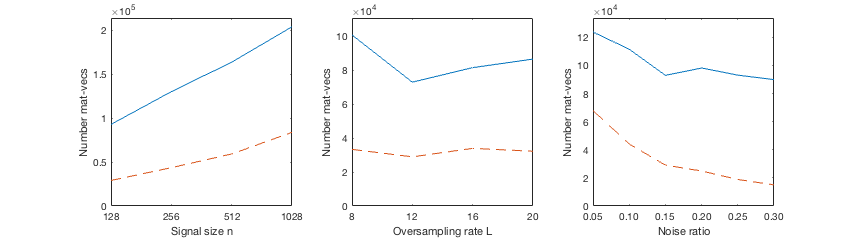
\includegraphics[scale=0.6]{Numerics-ada_vs_orig_various_params}
			}
	\vspace{0.0cm}
	\caption{
	Performance results for PLGD models with Gaussian noise (\ref{Eqn:PhaseLift-GD_Gaussian_noise}), where signals are complex with standard Gaussian distribution (\ref{Def:Gaussian_distribution_complex}).
	Results indicate Algorithm \ref{Alg:adaptive_IRAM} (dashed line) and the original IRAM parameters $m=20$, $r = 2$ (solid line). 
	Each result is the mean of 10 experiments.
	Left: Varying signal size $n$, with fixed noise ratio $\epsilon_\text{rel} = 0.15$ and oversampling scaled logarithmically with $n$ (i.e., $L = 10, 12, 12, 14$) as indicated in Theorem \ref{Thm:PhaseLift_approx}.
	Middle: Varying oversampling rate $L$, with fixed signal size $n = 128$ and noise ratio $\epsilon_\text{rel} = 0.15$.
	Right: Varying noise ratio $\epsilon_\text{rel}$, with fixed signal size $n = 128$ and oversampling rate $L = 10$.
	}
\label{Fig:Numerics-ada_vs_orig_various_params}
\end{figure}
% experiments.figure.noisyimage_comparison_adaptive_vs_orig

Figure \ref{Fig:Numerics-ada_vs_orig_various_params} demonstrates that Algorithm \ref{Alg:adaptive_IRAM} requires fewer matrix-vector products than the original IRAM parameters for the \emep \ for a wide range of phase retrieval problems.
The left and middle plots in Figure \ref{Fig:Numerics-ada_vs_orig_various_params} suggest that Algorithm \ref{Alg:adaptive_IRAM} requires about $60\%$ fewer matrix-vector products regardless of signal size $n$ or oversampling rate $L$.
Additionally, the right plot in Figure \ref{Fig:Numerics-ada_vs_orig_various_params} suggests Algorithm \ref{Alg:adaptive_IRAM} may reduce matrix-vector products by $80\%$ or more for problems with significant noise.


We also find that Algorithm \ref{Alg:adaptive_IRAM} is more efficient than the original IRAM settings for image-based phase retrieval problems.
Table \ref{Tab:Numerics-ada_vs_orig_large_images} shows the performance results for two larger images from Figure \ref{Fig:Numerics-large_images}.



\begin{table}[H]
\centering
\begin{tabular}{ |ccc|c|cc|cc| }
 \hline
			&&&  Original
			&  \multicolumn{2}{c|}{Algorithm \ref{Alg:adaptive_IRAM}}
			&	\multicolumn{2}{c|}{Algorithm \ref{Alg:adaptive_IRAM}}	\\
Image & $n$ & $L$ & $r=2, m=20$	& \multicolumn{2}{c|}{$m=40$}  & \multicolumn{2}{c|}{$m=80$}   \\
 \hline
	\multirow{2}{*}{Figure \ref{Fig:Numerics-large_images}, left} &
   \multirow{2}{*}{$57,600$} &  10 &  562,255  &  297,767 & 47\% &  252,316 & 55\% \\ 
  &&  15 &  647,753  &  301,752 & 53\% &  253,209 & 61\% \\ 
	\multirow{2}{*}{Figure \ref{Fig:Numerics-large_images}, right}  &   
     \multirow{2}{*}{$120,000$} &  10 &  852,633  &  364,164 & 57\% &  287,309 & 66\% \\ 
  &&  15 &  563,085  &  291,630 & 48\% &  256,084 & 55\% \\ 
 \hline
\end{tabular}
\caption{
Performance results for PLGD models with Gaussian noise (\ref{Eqn:PhaseLift-GD_Gaussian_noise}), where signals are the images in Figure \ref{Fig:Numerics-large_images}.
Results indicate total number of matrix-vector products and percent decrease from the original IRAM parameters.
Parameter $r$ is the number of requested eigenvalues in the IRAM (Algorithm \ref{Alg:IRAM}) and $m$ is the Arnoldi decomposition size (\ref{Eqn:Arnoldi_decomp}).
	} 
	\label{Tab:Numerics-ada_vs_orig_large_images}
\end{table}
% experiments.figure.noisyimage_comparison_adaptive_vs_orig



\begin{figure}[H]
\centering
	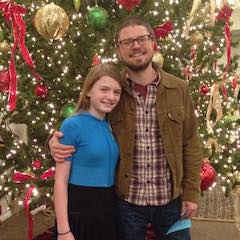
\includegraphics[scale=0.4166666666]{jul_and_me_orig}
		\hspace{0.1cm}
		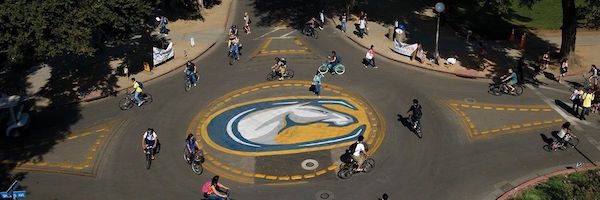
\includegraphics[scale=0.5]{UCD_orig}
		\vspace{0.3cm} \hspace{0.02cm}
		\\
	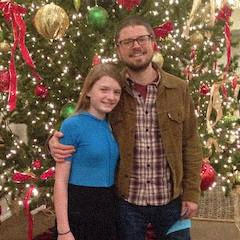
\includegraphics[scale=0.4166666666]{jul_and_me_L_15_ada40}	
		\hspace{0.1cm}
		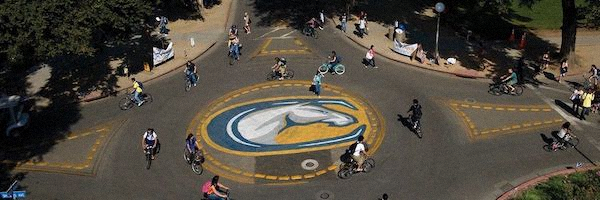
\includegraphics[scale=0.5]{UCD_L_15_ada40} 
		\vspace{0.0cm}
	\caption{
Images used for experiments in Table \ref{Tab:Numerics-ada_vs_orig_large_images}.
Top left: original image of my daughter and me, image size $240 \times 240 = 57,600$ pixels.
Bottom left: result image after solving EMEP.
Top right: original image of UC Davis roundabout, image size $200 \times 600 = 120,000$ pixels.
Bottom right: result image after solving EMEP.
All experiments have noise ratio $\epsilon_\text{rel} = 0.15$ and oversampling $L = 15$.
	}
\label{Fig:Numerics-large_images}
\end{figure}
% experiments.figure.noisyimage_comparison_adaptive_vs_orig


Table \ref{Tab:Numerics-ada_vs_orig_large_images} demonstrates that the benefits of Algorithm \ref{Alg:adaptive_IRAM} also apply to large-scale phase retrieval problems.
Additionally, a larger Arnoldi decomposition size $m$ further reduces the number of matrix-vector products.
Thus, when solving large-scale problems it may be advisable to consider increasing this parameter beyond the default setting of $m=40$ in Algorithm \ref{Alg:adaptive_IRAM} if memory constraints permit this increase.



Next, we demonstrate that Algorithm \ref{Alg:adaptive_IRAM} is nearly optimal in the sense of choosing the number of requested eigenvalues $r_k$ which minimizes the number of matrix-vector products for each \emep \ iterate $k$.
Table \ref{Tab:Numerics-num_matvecs_opt_vs_ada} indicates the number of matrix-vector products for solving the EMEP for six PLGD models with Gaussian noise (\ref{Eqn:PhaseLift-GD_Gaussian_noise}) with Algorithm \ref{Alg:adaptive_IRAM}, with the original IRAM parameters, and with the minimum possible number of matrix-vector products if each value $r_k$ was chosen such that $2 \leq r_k\leq 30$ and $r_k$ corresponds to the minimum number of matrix-vector products for the IRAM to evaluate EMEP iterate $k$.


\begin{table}[H]
\centering
\begin{tabular}{ |ccc|c|cc|cc| }
 \hline
			&&&  Original
			&  \multicolumn{2}{c|}{Optimal $2 \leq r \leq 30$}
			&	\multicolumn{2}{c|}{Algorithm \ref{Alg:adaptive_IRAM}}	\\
$L$ & $\epsilon_\text{rel}$ & EMEP its & $r=2, m=20$	& \multicolumn{2}{c|}{$m=40$}  & \multicolumn{2}{c|}{$m=40$}   \\
 \hline
 5 &  0.05 & 300 &  406,308  &  179,807 & 56\% &  198,070 & 51\% \\ 
  5 &  0.15 & 300 & 1,099,045  &  242,003 & 78\% &  258,385 & 76\% \\ 
  5 &  0.30 &  92 &  444,697  &   58,780 & 87\% &   69,510 & 84\% \\ 
 10 &  0.05 & 153 &   80,453  &   61,948 & 23\% &   68,709 & 15\% \\ 
 10 &  0.15 & 108 &   88,317  &   51,311 & 42\% &   57,231 & 35\% \\ 
 10 &  0.30 &  54 &   72,486  &   23,217 & 68\% &   25,809 & 64\% \\ 
 \hline
\end{tabular}

\caption{
Performance results for PLGD models with Gaussian noise (\ref{Eqn:PhaseLift-GD_Gaussian_noise}) with original signal from Figure \ref{Fig:parrot_signal_iterates} resized to $64 \times 64$ pixels.
Results indicate total number of matrix-vector products and percent decrease from the original IRAM parameters.
Parameter $r$ is the number of requested eigenvalues in the IRAM (Algorithm \ref{Alg:IRAM}) and $m$ is the Arnoldi decomposition size (\ref{Eqn:Arnoldi_decomp}).
} \label{Tab:Numerics-num_matvecs_opt_vs_ada}
\end{table}
% experiments.figure.noisyimage_adaptive_eig_full_exp

Table \ref{Tab:Numerics-num_matvecs_opt_vs_ada} demonstrates that Algorithm \ref{Alg:adaptive_IRAM} decreases the number of matrix-vector products of each PLGD model with Gaussian noise (\ref{Eqn:PhaseLift-GD_Gaussian_noise}) from the original IRAM parameters by a percentage comparable to that of the optimal choice for parameter $r$.
Notably, Algorithm \ref{Alg:adaptive_IRAM} is particularly effective at decreasing the number of matrix-vector products when there is a large relative difference between the number of matrix-vector products for the original IRAM parameters and the optimal parameters.
To further explore this performance behavior, Figure \ref{Fig:Numerics-num_eigs_ada_vs_opt} depicts the two PLGD models from Table \ref{Tab:Numerics-num_matvecs_opt_vs_ada} with the largest and smallest relative difference in matrix-vector products (those with $L=5$, $\epsilon_\text{rel} = 0.15$, and $L=10$, $\epsilon_\text{rel} = 0.05$, respectively).



\begin{figure}[H]
\centering
\hbox{\hspace{-1.8cm} 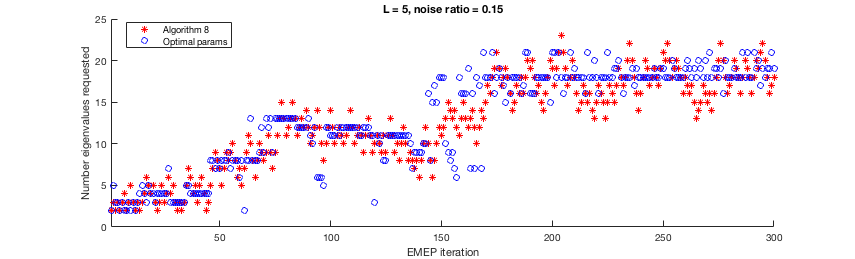
\includegraphics[scale=0.6]{Numerics-num_eigs_ada_vs_opt_1} }\vspace{0.6cm}
\hbox{\hspace{-1.8cm} 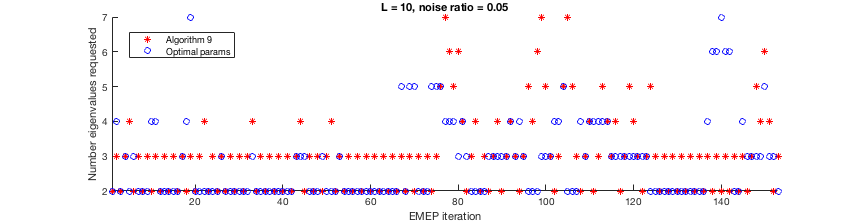
\includegraphics[scale=0.6]{Numerics-num_eigs_ada_vs_opt_2} }
\vspace{0.2cm}
	\caption{
	Number of requested eigenvalues $r$ in the IRAM (Algorithm \ref{Alg:IRAM}) for two PLGD models from Table \ref{Tab:Numerics-num_matvecs_opt_vs_ada}.
	}
\label{Fig:Numerics-num_eigs_ada_vs_opt}
\end{figure}
% experiments.figure.noisyimage_adaptive_eig_full_exp


In both PLGD models depicted in Figure \ref{Fig:Numerics-num_eigs_ada_vs_opt}, the number of requested eigenvalues $r$ chosen by Algorithm \ref{Alg:adaptive_IRAM} is usually within 1-3 units from the optimal parameter value.
The bottom plot in Figure \ref{Fig:Numerics-num_eigs_ada_vs_opt} suggests that Algorithm \ref{Alg:adaptive_IRAM} required relatively more matrix-vector products than the optimal value of $r$ because Algorithm \ref{Alg:adaptive_IRAM} always changes the value of $r$ by one or two units, thus shifting away from the optimal value $r=2$ for many EMEP iterates.
As we saw in Figure \ref{Fig:Numerics-surf_mvs_eig_diffs_2}, the optimal parameter $r$ may shift rapidly for some PLGD models, and thus Algorithm \ref{Alg:adaptive_IRAM} always changes $r$ by one or two units to continue gathering performance information about the EMEP.



%\subsection{Performance results for varying Arnoldi decomposition size}				



Finally, we use performance results to justify selecting $m=40$ as the default Arnoldi decomposition (\ref{Eqn:Arnoldi_decomp}) size for Algorithm \ref{Alg:adaptive_IRAM}.
Table \ref{Tab:Numerics-num_matvecs_orig_vs_ada} depicts the total number of matrix-vector products required to solve the \emep \ for each PLGD model from Table \ref{Tab:Numerics-num_matvecs_opt_vs_ada} with Algorithm \ref{Alg:adaptive_IRAM} with various parameter values $m$.

\begin{table}[H]
\centering
\begin{tabular}{ |ccc|c|ccccc| }
 \hline
			  \multicolumn{3}{|c|}{n = 4,096} &  Original
			&  \multicolumn{5}{c|}{Algorithm \ref{Alg:adaptive_IRAM}}	\\
$L$ & $\epsilon_\text{rel}$ & EMEP its & $r=2, m=20$	& $m=20$  & $m=40$  & $m=60$  & $m=80$  & $m=100$   \\
 \hline
  5 &  0.05 & 300 &  406,308  &  358,195  &  198,070  &  189,401  &  192,042  &  201,270  \\ 
  5 &  0.15 & 300 & 1,099,045  &  806,412  &  258,385  &  224,048  &  214,118  &  215,392  \\ 
  5 &  0.30 &  92 &  444,697  &  175,669  &   69,510  &   56,193  &   55,146  &   54,987  \\ 
 10 &  0.05 & 153 &   80,453  &   77,768  &   68,709  &   64,300  &   68,602  &   73,754  \\ 
 10 &  0.15 & 108 &   88,317  &   65,833  &   57,231  &   53,261  &   54,388  &   55,308  \\ 
 10 &  0.30 &  54 &   72,486  &   28,799  &   25,809  &   24,699  &   25,113  &   25,491  \\ 
 \hline
\end{tabular}

\caption{
Total number of matrix-vector products for various PLGD models with Gaussian noise	(\ref{Eqn:PhaseLift-GD_Gaussian_noise}) with original signal from Figure \ref{Fig:parrot_signal_iterates} resized to $64 \times 64$ pixels.
Parameter $r$ is the number of requested eigenvalues in the IRAM (Algorithm \ref{Alg:IRAM}) and $m$ is the Arnoldi decomposition (\ref{Eqn:Arnoldi_decomp}) size. 
} \label{Tab:Numerics-num_matvecs_orig_vs_ada}
\end{table}
% experiments.figure.noisyimage_adaptive_eig_full_exp



Table \ref{Tab:Numerics-num_matvecs_orig_vs_ada} demonstrates that Algorithm \ref{Alg:adaptive_IRAM} reduces the number of matrix-vector products from those of the original IRAM parameters for all experiments considered.
Yet this cost reduction varies significantly depending on the choice of Arnoldi decomposition (\ref{Eqn:Arnoldi_decomp}) size $m$.
We seek a default setting for the parameter $m$ which is sufficiently large to yield the benefits of Algorithm \ref{Alg:adaptive_IRAM}, yet sufficiently small as not to impact memory constraints.
To select an appropriate default value for $m$, we examine the two experiments from Table \ref{Tab:Numerics-num_matvecs_orig_vs_ada} with $\epsilon_\text{rel} = 0.15, 0.30$ and $L=5$ which have the greatest original number of matrix-vector products, along with the greatest total decrease in cost when using Algorithm \ref{Alg:adaptive_IRAM} with a sufficiently large parameter $m$.
Figure \ref{Fig:Numerics-num_matvecs_ada_for_m_vals} singles out these two experiments, depicting the number of matrix-vector products for each \emep \ iteration.

\begin{figure}[H]
\centering
\hbox{\hspace{-1.6cm} 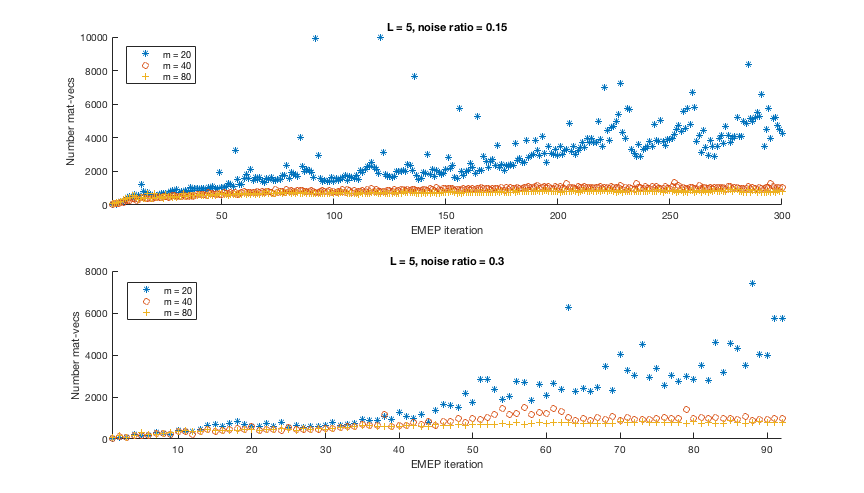
\includegraphics[scale=0.6]{Numerics-num_matvecs_ada_for_m_vals} }\vspace{0.0cm}
	\caption{Number of matrix-vector products for each \emep \ iteration from two experiments in Figure \ref{Fig:Numerics-num_matvecs_ada_for_m_vals} with various Arnoldi decomposition size $m=20, 40, 80$.}
\label{Fig:Numerics-num_matvecs_ada_for_m_vals}
\end{figure}
% experiments.figure.noisyimage_adaptive_eig_full_exp




Figure \ref{Fig:Numerics-num_matvecs_ada_for_m_vals} demonstrates that the Arnoldi decomposition size of $m=20$ is not sufficiently large to allow Algorithm \ref{Alg:adaptive_IRAM} to decrease the number of matrix-vector products.  
The dramatic matrix-vector product spikes for $m=20$ in Figure \ref{Fig:Numerics-num_matvecs_ada_for_m_vals} resemble those first seen in Figure \ref{Fig:EMEP_costs_num_mat_vecs} when solving the \emep \ with the original IRAM parameters $m=20, r=2$.
Yet when the Arnoldi decomposition size is increased to $m=40$, these cost spikes effectively disappear.
The change in number of matrix-vector products between $m=40$ and $m=80$ is minimal for each EMEP iterate.  
Thus the default parameter of $m=40$ for Algorithm \ref{Alg:adaptive_IRAM} strikes the proper balance between efficiency and memory constraints.












      
\newpage

   

\chapter{Conclusion}			\label{Sec:Conclusion}


In this dissertation we examined noisy phase retrieval, focusing on the PLGD model (\ref{Eqn:PhaseLift-P-GD}) which we chose to optimize with the Gauge Dual Descent (GDD) algorithm (Algorithm \ref{Alg:PGD} from Chapter \ref{Sec:PLGD_algo}).
Section \ref{Subsec:Conclusion-contrib} summarizes our contributions and Section \ref{Subsec:Conclusion-future} discusses some theoretical and computational questions which remain for future work.




\section{Contributions}		\label{Subsec:Conclusion-contrib}


Our work provides two main contributions which lead to the development of the Improved Gauge Dual Descent (IGDD) algorithm (Algorithm \ref{Alg:PGD-improved}).


The first main contribution was to establish new termination conditions (\ref{Eqn:term_crit_new-primal_difference}) and (\ref{Eqn:term_crit_new-dual_difference}) for the GDD algorithm.
Chapter \ref{Sec:PLGD_term_crit} showed that PLGD models with Gaussian noise (\ref{Eqn:PhaseLift-GD_Gaussian_noise}) cause the GDD algorithm to stagnate prior to satisfying the original termination conditions (\ref{Eqn:saga_conv_crit_primal}) and (\ref{Eqn:saga_conv_crit_gap}).  
We saw that this stagnation was likely the result of the optimal PLGD matrix $\caA^*y_\star$ having an algebraically largest eigenvalue with multiplicity greater than one.
Thus the objective function $\lambda_1(\caA^*y)$ will be nondifferentiable in the neighborhood of $y_\star$ and we may expect first-order methods like the GDD algorithm to stagnate in this neighborhood.
As a result, we established new termination conditions (\ref{Eqn:term_crit_new-primal_difference}) and (\ref{Eqn:term_crit_new-dual_difference}) based on empirical evidence of algorithmic stagnation.


The second main contribution was to develop a new strategy for handling the \emep \ in the GDD algorithm.
In Chapter \ref{Sec:evol_mats} we defined the EMEP in the GDD algorithm and examined the evolving spectrum of the EMEP.
We observed that the algebraically largest eigenvalues of the EMEP tend to cluster for later iterates, making these eigenvalue problems more difficult for methods like the IRAM (Algorithm \ref{Alg:IRAM}).
We also showed that the EMEP is the computational bottleneck of the GDD algorithm, requiring about $95$\% of the matrix-vector products in the GDD algorithm.
Section \ref{Subsec:evol_mats-IRAM} then reviewed the IRAM and its component algorithms, providing insight for how we may better select the IRAM parameters.
In Section \ref{Subsec:evol_mats-adaptive_IRAM} we developed Algorithm \ref{Alg:adaptive_IRAM}, a new strategy for solving the EMEP by selecting the number of requested eigenvalues in the IRAM based on empirical observations of IRAM behavior.
Section \ref{Subsec:evol_mats-correl_btwn_EMEP_and_IRAM} showed that changes in the number of requested eigenvalues, as chosen by Algorithm \ref{Alg:adaptive_IRAM}, correspond to clustering of the algebraically largest eigenvalues in the EMEP.


In Chapter \ref{Sec:Numerics} we presented the IGDD algorithm which incorporates the new termination conditions of Chapter \ref{Sec:PLGD_term_crit} and the new strategy for the EMEP from Chapter \ref{Sec:evol_mats}.
Performance results demonstrated that the IGDD algorithm is more efficient than the GDD algorithm for a variety of noisy phase retrieval problems.
In particular, the IGDD algorithm typically reduced the number of matrix-vector products by $50$-$80\%$ for problems with a low oversampling rate.


In addition to these main contributions, Chapter \ref{Sec:PLGD} presented a self-contained, comprehensive treatment of gauge duality theory for establishing and analyzing the PLP-PLGD pair.
Also, Appendix \ref{Sec:Appx-Comparison} examined some of the benefits of choosing the PLGD model (\ref{Eqn:PhaseLift-P-GD}) for noisy phase retrieval.
We saw that the PLGD model is well-suited for developing a first-order method, and that the GDD algorithm typically solves noisy phase retrieval problems with greater accuracy than the wflow algorithm (Algorithm \ref{Alg:wflow}).



\section{Future Work}		\label{Subsec:Conclusion-future}

Several theoretical and computational questions still remain for future work.  
In terms of theory, it would be beneficial to determine the expected rank of the optimal PLGD matrix $\caA^*y_\star$ for a given noisy phase retrieval problem. 
As shown in Chapter \ref{Sec:PLGD_term_crit}, PLGD models with Gaussian noise typically have optimal matrices $\caA^*y_\star$ with rank $\rho$ greater than one (see Table \ref{Tab:average_rank_soln_matrix_with_gaussian_dual_variable}).
Thus, as the GDD algorithm progresses we may expect the $\rho$ algebraically largest eigenvalues of $\caA^*y$ to cluster.
Algorithm \ref{Alg:adaptive_IRAM} changes the number of requested eigenvalues $r$ in the IRAM (Algorithm \ref{Alg:IRAM}) as the spectrum of $\caA^*y$ evolves.
As we saw in Section \ref{Subsec:evol_mats-correl_btwn_EMEP_and_IRAM}, changes in the choice of $r$ appear to correlate with clustering of the algebraically largest eigenvalues of $\caA^*y$.
In this sense, the value $r$ selected by Algorithm \ref{Alg:adaptive_IRAM} may be a proxy for determining the rank $\rho$ of $\caA^*y_\star$.
Knowledge of the expected value for $\rho$ may provide both theoretical justification for Algorithm \ref{Alg:adaptive_IRAM} and a means to improve Algorithm \ref{Alg:adaptive_IRAM}.


Many computational questions also remain for future work.
In terms of solving the \emep, we did not examine parallel methods for solving this sequence of problems.\footnote{
Note that we did consider the \textit{inverse free preconditioned Krylov subspace method} (EIGIFP) \cite{golub2002inverse}, which was comparable to or slightly slower than IRAM.  EIGIFP is implemented in MATLAB and this code had some numerical issues for larger PLGD models.
}
We also did not discuss optimizing the method for handling the primal recovery problem (\ref{Eqn:GD-PFD}) in the GDD algorithm.
Recall that the primal recovery problem requires $2$-$5\%$ of the total DFTs in a given PLGD model (see Table \ref{Tab:EMEP_costs}).
The current method used is \textit{minFunc} \cite{schmidt2005minFunc}, which is a quasi-Newton method based only on gradient information.
However, a recent paper \cite{sun2016geometric} indicates that the objective function in (\ref{Eqn:GD-PFD}) has no spurious local minima and negative directional curvature at all saddle points.
Thus the Hessian of this function may also be used to solve (\ref{Eqn:GD-PFD}).
Finally, we did not discuss alternative methods to the GDD algorithm for optimizing the PLGD model itself.\footnote{
Note that we did consider \textit{minConf} \cite{schmidt2008minConf}, a descent method for problems like the PLGD model with an expensive objective function and cheap projection operator.  This method appeared comparable to the GDD algorithm and in some cases faster.
}







\newpage


\appendix



\chapter{Proof of PhaseLift-$l_1$ Gauge Duality in Section \ref{Subsec:phase_retrieval-why_optimize_PLGD_model}} 	\label{Sec:Appx-PL-l1}

In this appendix we show that the following pair of PhaseLift-$l_1$ models discussed in Section \ref{Subsec:phase_retrieval-why_optimize_PLGD_model} are a primal and gauge dual pair
\begin{equation}				\label{Eqn:PhaseLift_l-1_norm_model_gauge_dual}
\begin{array}{llllll}
	&\min
	& ||\caA(X) - b||_1
		&&\min\limits_{y}
			&	||y||_\infty
		\\
\textnormal{(PLP-}l_1) &	\st
	&	X \succeq 0
		& \textnormal{(PLGD-}l_1)		
		&	\st
			&	-\caA^*y \succeq 0
		\\
	&&&&&	\langle b, y \rangle \geq 1.
\end{array}
\end{equation}

To determine the gauge dual of PLP-$l_1$, first note that the objective function $f(X) = ||\caA(X) - b||_1$ is not a gauge function, as $f$ is not positively homogeneous.  Using the substitution $z = b - \caA(X)$ and extending the linear operator $\caA$, we may restate PLP-$l_1$ as
\begin{equation} 		\label{Eqn:PhaseLift_l-1_norm_model_general}
\begin{array}{ll}
\min\limits_{X, z}
	&	\kappa(X, z) := ||z||_1 + \delta_{\succeq 0}(X)
		\\
\st
	&	\overline{\caA}(X, z) := \caA(X) + z = b,
\end{array}
\end{equation}
which is now in the form of (\ref{Eqn:PhaseLift_P_GD_inequality_form}).  The gauge functions $\kappa_1(z) = ||z||_1$ and $\kappa_2(X) = \delta_{\succeq 0}(X)$ have polars $\kappa_1^\circ(w) = ||w||_\infty$ and $\kappa_2^\circ(V) = \delta_{\succeq 0}(-V)$.  Thus, by Proposition \ref{Prop:P-GD-polar_of_sum_of_gauges}, $\kappa$ has the polar
\begin{equation}
\kappa^\circ(V, w) = \max \{ ||w||_\infty, \ \delta_{\succeq 0}(-V) \} = ||w||_\infty + \delta_{\succeq 0}(-V).
\end{equation}
Additionally, the adjoint of $\overline{\caA}$ is $\overline{\caA}^*y = (\caA^*y, y)$, giving
\begin{equation}
\kappa^\circ(\overline{\caA}^*y) = ||y||_\infty + \delta_{\succeq 0}(-\caA^*y).
\end{equation}
Passing $\delta_{\succeq 0}(-\caA^*y)$ into the constraint set, we see that PLGD-$l_1$ is the gauge dual of PLP-$l_1$.

\newpage



\chapter{Further justification of residuals established in Chapter \ref{Sec:PLGD_term_crit}}      		\label{Sec:Appx-further_reasons_for_new_term_crit}


\begin{enumerate}



\item

The previous section demonstrated that the primal difference (\ref{Eqn:term_crit-candidate_residuals}e) and dual variable difference (\ref{Eqn:term_crit-candidate_residuals}i) effectively identify the point at which Algorithm \ref{Alg:PGD} stagnates for PLGD models with Gaussian noise (\ref{Eqn:PhaseLift-GD_Gaussian_noise}).  We close this chapter with a justification for ignoring the remaining residuals (\ref{Eqn:term_crit-candidate_residuals}).  As we will see, each of these residuals is either unreliable or effectively a duplicate of another (computationally cheaper) residual.  

One residual that may be eliminated is the primal relative error (\ref{Eqn:term_crit-candidate_residuals}d).  The original termination conditions for Algorithm \ref{Alg:PGD} include the feasibility requirement (\ref{Eqn:saga_conv_crit_primal}) 
\begin{equation*}
|| \caA(xx^*) - b || \leq \epsilon + \textnormal{tol}_\textnormal{feas} (1 + ||b||),
\end{equation*}
which is equivalent to the primal relative error (\ref{Eqn:term_crit-candidate_residuals}d) using the relation $\epsilon_\rel = \epsilon / ||b||$
\begin{equation}
	\label{Eqn:GD_new_termination_conds-primal_feas}
\frac{||\caA(xx^*) - b||}{||b||}  \leq \epsilon_\rel + \textnormal{tol}_\textnormal{feas} \left(\frac{1 + ||b||}{||b||}\right).
\end{equation}
As indicated in Table \ref{Tab:term_crit-pr_feas_faster_for_big_L_noise}, Algorithm \ref{Alg:PGD} typically requires only a few iterations before a primal feasible signal $x$ is found.  Yet in certain cases this algorithm may never identify a feasible signal.  Figure \ref{Fig:term_crit-pr_err_fails} demonstrates plots the primal relative error (\ref{Eqn:term_crit-candidate_residuals}d) for the particular model from Figure \ref{Fig:term_crit-signal_err} which never attained primal feasibility.

\begin{figure}[H]
\centering
\hbox{\hspace{-1.6cm} 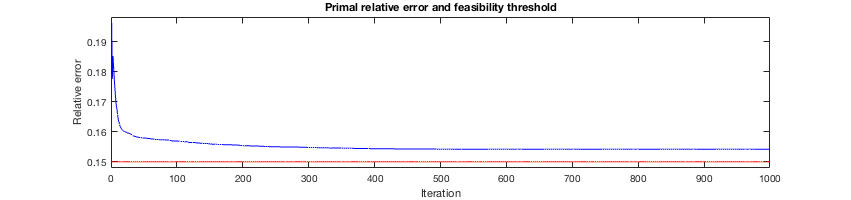
\includegraphics[scale=0.6]{term_crit-pr_err_fails} }
\caption{Primal relative error (\ref{Eqn:term_crit-candidate_residuals}d) (blue) and noise ratio threshold (red) for noise ratio $\epsilon_\rel = 0.15$ and oversampling rate $L = 5$.  Iterate 1,000 remains infeasible with a primal relative error of $0.1541$.}
\label{Fig:term_crit-pr_err_fails}
\end{figure}

% experiments.figure.noisyimage_new_termination_criteria

The experiment in Figure \ref{Fig:term_crit-pr_err_fails} demonstrates a model where both the exact tolerance $\epsilon_\rel = 0.15$ and the relaxed tolerance $ \epsilon_\rel + \textnormal{tol}_\textnormal{feas} \left(\frac{1 + ||b||}{||b||}\right) =0.1502$ as suggested in (\ref{Eqn:saga_conv_crit_primal}) are unattainable by Algorithm \ref{Alg:PGD}.  Nevertheless, this algorithm makes significant progress in recovering an approximate signal.  Notably, wflow applied to the same model recovers a signal with a primal relative error (\ref{Eqn:term_crit-candidate_residuals}d) of $0.3165$.  Thus we ignore the primal feasibility condition (\ref{Eqn:saga_conv_crit_primal}).


We may also disregard the duality gap (\ref{Eqn:term_crit-candidate_residuals}f) as a termination condition.  The experiments in Table \ref{Tab:average_rank_soln_matrix_with_gaussian_dual_variable} demonstrate that the duality gap tends to stagnate at different values for differing noise level and oversampling rate.  Table \ref{Tab:term_crit-duality_gap_stagnates} indicates the final duality gap value for each experiment from Figure \ref{Fig:term_crit-signal_err}, further demonstrating this residual is not a reliable indicator of stagnation.

\begin{table}[H]
\centering
\begin{tabular}{ |c|c|c| }
\hline
&	$L = 5$
	&	$L = 10$	\\
 \hline
$\epsilon_\rel = 0.05$
&     8.24 &   8.10 		\\
 \hline
$\epsilon_\rel = 0.15$
&  39.23 &  29.41 	\\
 \hline
$\epsilon_\rel = 0.30$
&  38.93 &  59.73	\\
 \hline
\end{tabular}
	\caption{Final values of duality gap (\ref{Eqn:term_crit-candidate_residuals}f) after 1,000 iterations of Algorithm \ref{Alg:PGD} with indicated noise ratios and oversampling rates.}
	\label{Tab:term_crit-duality_gap_stagnates}
\end{table}
% experiments.figure.noisyimage_new_termination_criteria

The duality gap (\ref{Eqn:term_crit-candidate_residuals}f) is not reliable because this measurement is dependent on the accuracy of both the dual objective value $\lambda_1$ and the approximate signal norm $||xx^*||_1$ as compared to their respective optimal values.  As established in Section \ref{Subsec:PLGD_term_crit-stagnation}, Algorithm \ref{Alg:PGD} cannot achieve optimality for most noisy phase retrieval models.  Thus the complementarity condition $||xx^*||_1 \cdot \lambda_1 = 1$ (Corollary \ref{Cor:PLGD-optimality}, d) cannot be achieved.  As a result, the duality gap (\ref{Eqn:term_crit-candidate_residuals}f) stagnates unpredictably for varying oversampling rates and noise levels and is not used as a termination condition for Algorithm \ref{Alg:PGD}.



Next we demonstrate that the duality gap difference (\ref{Eqn:term_crit-candidate_residuals}g) is a redundant measurement.  Denote the primal objective value as $p = ||xx^*||_1$ and its update with a hat.  As Algorithm \ref{Alg:PGD} stagnates, $\hat{p} / p$ approaches $1$. Additionally, note that typical optimal signals have fairly large norms (i.e., $||\bar{x}\bar{x}^*||_F = \caO(10^3)$ or larger).  If we assume $\hat{p}/p \approx 1$ and $\lambda_1 -  1/p \approx \lambda_1$ for later iterates then we have
\begin{equation}
\begin{split}
\frac{| \gamma - \hat{\gamma}|}{\gamma}	&	=	\frac{| (p \lambda_1 - 1) - (\hat{p}\hat{\lambda}_1 - 1) |}{p \lambda_1 - 1}
		\\
	&	= \frac{\left| \lambda_1 - \frac{\hat{p}}{p}\hat{\lambda}_1 \right|}{ \lambda_1 - \frac{1}{p} }
		\\
	&	\approx \frac{| \lambda_1 - \hat{\lambda}_1|}{\lambda_1}.
\end{split}
\end{equation}

Thus the duality gap difference (\ref{Eqn:term_crit-candidate_residuals}g) behaves similarly to the dual objective difference (\ref{Eqn:term_crit-candidate_residuals}h) and may be disregarded.  

Finally, the dual matrix difference (\ref{Eqn:term_crit-candidate_residuals}j) is also a redundant measurement which may be disregarded.  Note that the norm difference of dual matrices is bounded above by the dual variable difference (\ref{Eqn:term_crit-candidate_residuals}i), since
\[
||A - \hat{A}||_F = ||\caA^*(y - \hat{y})||_F \leq ||\caA^*|| \ ||y - \hat{y}||,
\]
where we have the induced norm
\[
||\caA^*|| = \sup_{\substack{||w||=1}}||\caA^*w||_F.
\]
And computationally, the dual variable difference (\ref{Eqn:term_crit-candidate_residuals}i) is computed with a vector norm, where as the dual matrix difference (\ref{Eqn:term_crit-candidate_residuals}j) requires an additional eigenvalue computation (in this case the largest magnitude eigenvalue).  Thus the dual matrix difference (\ref{Eqn:term_crit-candidate_residuals}j) can be ignored due to its excessive computational cost and close relationship to the dual variable difference (\ref{Eqn:term_crit-candidate_residuals}i).



Finally, we may also eliminate the dual objective difference (\ref{Eqn:term_crit-candidate_residuals}h) as a candidate residual for termination.  Figure \ref{Fig:term_crit-dual_obj} depicts the behavior of this residual for the models in Figure \ref{Fig:term_crit-signal_err}.  As with Figure \ref{Fig:term_crit-pr_and_dual}, the vertical axis indicates specific tolerances and the horizontal axis indicates the first iterate at which Algorithm \ref{Alg:PGD} would satisfy this tolerance.


\begin{figure}[H]
\centering
\hbox{\hspace{-2.1cm} 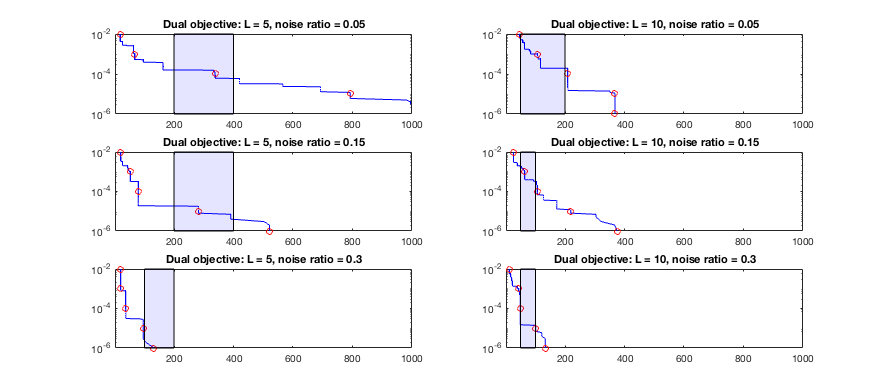
\includegraphics[scale=0.6]{term_crit-dual_obj} }\vspace{-0.4cm}
\caption{Plots of dual objective difference values (\ref{Eqn:term_crit-candidate_residuals}h) against the iterate at which Algorithm \ref{Alg:PGD} first satisfies this tolerance for the models discussed in Figure \ref{Fig:term_crit-signal_err}.  Red circles are placed at tolerances $10^{-n}$.  The blue rectangles indicate the proposed intervals of termination from Table \ref{Tab:term_crit-desired_termination_windows}.}
\label{Fig:term_crit-dual_obj}
\end{figure}
% experiments.figure.noisyimage_new_termination_criteria


Figure \ref{Fig:term_crit-dual_obj} demonstrates that the dual objective difference (\ref{Eqn:term_crit-candidate_residuals}h) behaves erratically, decreasing too slowly for low-noise models and too quickly for high-noise models.  To simplify our discussion, label the dual objective tolerance as $\tol_\text{DO}$.  If we set $\tol_\text{DO} = 10^{-5}$, then Algorithm \ref{Alg:PGD} will terminate far too late for the top-left model in Figure \ref{Fig:term_crit-dual_obj}.  However, if we set $\tol_\text{DO} = 10^{-4}$ then the algorithm may terminate far too early for the middle-left and bottom-left models.  Likewise, the models at right in Figure \ref{Fig:term_crit-dual_obj} do not have a consistent tolerance value $\tol_\text{DO}$ which reliably selects for termination within the desired intervals.  Thus the tolerance $\tol_\text{DO}$ is not a reliable indicator of stagnation of Algorithm \ref{Alg:PGD}.  


\end{enumerate}


\newpage



\bibliographystyle{amsalpha-fi-arxlast}
\bibliography{DissertationBibliography}


\end{document}
